%  History
%  04/11/16  JAM added some tidbits here and there
%  04/29/08  jcv few more final mods
%  01/27/08  jcv some modifications and simplifying
%  05/15/06  kg made available to UMD Astro Wiki
%  01/12/05  kg retrieved from DSR 
%  05/27/04  DSR  retrieved from Wayne Baumgartner
%

% Official version for University
% Also, do not use \makecover for official version.
\documentclass[12pt,letterpaper,oneside]{dissertation}

% Use the following instead of the above for duplex printing.
%  Makes ``inside'' margins 1.5 inches.  Also forces odd-numbered
%  pages to be on the right, and forces new chapters to be on
%  odd-numbered pages
%\documentclass[12pt,letterpaper,twoside]{dissertation}

%jam added this to get glossaries to work
% arara: pdflatex: { synctex: on, action: nonstopmode }
% arara: bibtex
% arara: makeglossaries
% arara: pdflatex: { synctex: on, action: nonstopmode }

\usepackage{longtable} 
\usepackage{subfigure}
\usepackage{graphicx}
\usepackage{ifthen}
\usepackage{epstopdf}
% To use AAS macros
\usepackage{sty/aastex_hack}
% Use improved verbatim package for included code and force single
% spacing in it.

\usepackage{fancyvrb}
\fvset{baselinestretch=1}
% Package to deal with acronyms nicely
\usepackage{acronym} %jam maybe comment this out?
%Jam added glossaries
%Jame trying to get deluxetable to play nice with glossaries which includes supertabular

%jam added lineno, not sure we need it?
\usepackage{lineno}
%\linenumbers

\usepackage[nomain,acronym,toc, nonumberlist]{glossaries}
\let\shead = \tablehead
\let\stail = \tabletail
\let\tablehead\relax
\let\tabletail\relax
\let\tablecaption\relax
\usepackage{sty/deluxetable}
\let\thead=\tablehead
\let\ttail=\tabletail
\let\tcap=\tablecaption
\let\tablehead =\thead
\let\tabletail =\ttail
\let\tablecaption =\tcap

\renewcommand*{\acronymname}{List of Symbols and Acronyms}
\loadglsentries{abbrev}
%%List of abbreviations
%\newacronym[longplural={Frames per Second}]{fpsLabel}{FPS}{Frame per Second}

%\newacronym{LAT}{name = {LAT}, text ={lare area telescope}, description ={ Large Area Telescope}}%simple example
%\newglossaryentry{uppercase}{
%	name={Uppercase},
%	text={uppercase},
%	description={Appears uppercase in the glossary and lowercase in the text}
%}

\newacronym{1FGL}{1FGL}{First Fermi LAT source catalog}
\newacronym{2FGL}{2FGL}{Second Fermi LAT source catalog}
\newacronym{3FGL}{3FGL}{Third Fermi LAT source catalog}
\newacronym{2FHL}{2FHL}{Second Catalog of Hard Fermi-LAT Sources}
\newacronym{ACD}{ACD}{anti-coincidence detector}
\newacronym{AGN}{AGN}{active galactic nucleus}
\newacronym{BPL}{BPL}{broken power law}
\newacronym{CGRO}{CGRO}{Compton Gamma-Ray Observatory}
\newacronym{CR}{CR}{cosmic ray}
\newacronym{CTA}{CTA}{Cherenkov Telescope Array}
\newacronym{DM}{DM}{dispersion Measure}
\newacronym{ECPL}{ECPL}{exponentially cut-off power law}
\newacronym{EGRET}{EGRET}{Energetic Gamma-Ray Experiment Telescope}
\newacronym{GBM}{GBM}{Gamma-ray Burst Monitor}
\newacronym{GRB}{GRB}{gamma-gay burst}
\newacronym{HE}{HE}{high energy}
\newacronym{IC}{IC}{inverse compton}
\newacronym{ISM}{ISM}{interstellar medium}
\newacronym{LAT}{LAT}{Large Area Telescope}
\newacronym{MAGIC}{MAGIC}{Major Atmospheric Gamma-ray Imaging Cherenkov telescopes}
\newacronym{MSP}{MSP}{millisecond pulsar}
\newacronym{NS}{NS}{neutron star}
\newacronym{PL}{PL}{power law}
\newacronym{PSR}{PSR}{pulsar}
\newacronym{PWN}{PWN}{pulsar wind nebula}
\newacronym{RoI}{RoI}{region of interest}
\newacronym{SNR}{SNR}{supernova remnant}
\newacronym{TS}{TS}{test statistic}
\newacronym{VERITAS}{VERITAS}{Very Energetic Radiation Imaging Telescope Array System}
\newacronym{VHE}{VHE}{very high energy}
\newacronym{MC}{MC}{molecular cloud}
\newacronym{SNRMC}{SNR-MC}{supernova remant molecular system}
%List of Symbols

\newglossaryentry{nh}
{
	name={\ensuremath{~\mathrm{N_{\rm{H}}}}},
	description={Neutral Hydrogen Number Density},
	sort=Nh
}

\makeglossaries
%jam not sure I need an index
%\usepackage[xindy]{imakeidx}
%\makeindex

% Instruction to natbib package to omit comma between name and date
% within citations as well as to do name-date citation style the sort
% option forces output of multiple items to be in the order that they
% show up in Bibliography.
\usepackage[authoryear,round,sort]{natbib}
\bibpunct{(}{)}{;}{a}{}{,}
\usepackage{sty/natbibspacing}

% Where I define my personal macros; probably should input this instead
\usepackage{sty/mydefs}

% To fiddle with captions
\usepackage[small]{caption}
% Instruction to caption.sty to make a 20pt margin on each side of
% captions
\setlength{\captionmargin}{20pt}
% To single space captions, tables, etc.
\usepackage{sty/atbeginend}

% To reduce the size of chapter, etc headings
\usepackage{sectsty}
\chapterfont{\huge\centering}
\usepackage[nobottomtitles]{titlesec}

\usepackage{pdfpages}
\usepackage{hyperref}
\hypersetup{
pdfauthor = {Jamie Michael Cohen},
pdftitle = {Doctor of Philosophy, 2016},
pdfsubject = {Subject Dissertation},
}
% Depth of section numbering in body 
%\setcounter{secnumdepth}{3}

% Fix spacing in floats
% atbeginend.sty stuff: (spacing commands defined in dissertation.sty)
\BeforeBegin{deluxetable}{\spacing{1}}
\AfterEnd{deluxetable}{\spacing{\bodyspacing}}
\BeforeBegin{table}{\spacing{1.1}}
\AfterEnd{table}{\spacing{\bodyspacing}}
\BeforeBegin{figure}{\spacing{1.1}}
\AfterEnd{figure}{\spacing{\bodyspacing}}
\BeforeBegin{figure*}{\spacing{1.1}}
\AfterEnd{figure*}{\spacing{\bodyspacing}}

% For intelligent float placement fiddle with these
\renewcommand{\topfraction}{0.9}
\renewcommand{\bottomfraction}{0.9}
\renewcommand{\floatpagefraction}{0.75}
\renewcommand{\textfraction}{0.1}
\renewcommand{\dbltopfraction}{0.75}
%\interfootnotelinepenalty=10000 %jam added to stop footnoes from bleeding o
% Make the front matter 
% Long titles need to have breaks forced within them with \\ at break.
\title{\g-Ray Studies of Stellar Graveyards: \\ Fermi-LAT Observations of Supernova Remnants \\
	 and Spatially Extended Emission \\}

\author{Jamie Michael Cohen} % You should really have full name here.
\date{2016} % Date of your degree.
\department{Astroparticle Physics Laboratory, Code 661 \\ NASA Goddard Space Flight Center}
\advisor{Doctor Elizabeth Hays}
\chairtitle{Chair/Advisor}
\advtitle{Advisor}
\chairdept{Department of Astronomy \\ University of Maryland}
\chairname{Professor M. Coleman Miller}
% Rest of committee in alphabetical order with title.  Any type of
% professor (assistant, associate, or adjunct) gets ``Professor.''
\committee{Professor Christopher S. Reynolds \\
                Professor Derek C. Richardson \\
                Professor Jordan Goodman, Dean's Representative}

% Comment out the following three lines if you don't want to dedicate
% your thesis, you uninspired piece of scum.
\phantomsection
\label{mydedication}
\dedication{\centering To Vanessa $\heartsuit$}

% Abstract is required for UMD as of 2006.
\abstractfile{abstract}

% Just comment out if you don't want to acknowledge anyone, you
% ungrateful little pipsqueak.
\acknowledgements{%I should probably thank someone because I'm not a degenerate.
%JAM: Added this from the example UMD ack

%\renewcommand{\baselinestretch}{2}
%\small\normalsize
%\hbox{\ }

%\vspace{-.65in}

%\begin{center}
%	\large{Acknowledgments} 
%\end{center} 

%\vspace{1ex}
I think anyone who has been through grad school knows that one lone grad student a dissertation does not make. There have been many people along the way who helped set me on this path, guided me through it, and  supported me throughout. I'd like to start this thesis properly by gushing about the awesomeness of my advisor, Liz Hays. Liz has been infinitely supportive, patient, and encouraging of me, especially in times of doubt (which are many in grad school). She has been a fount of knowledge and wisdom (both of the academic and non-academic variety), and is ever so deft at nudging me in the right directions while simultaneously allowing me to lead and figure things out on my own. If only a few of these qualities have rubbed off on me, I'd be a better person and scientist for it. I can't imagine going through and getting through this journey without her and I'm proud to be her first grad student. 

I am grateful to Cole Miller for being the head of my thesis committee and co-advisor. Cole's advice is always insightful and his steadfast confidence in my abilities has been invaluable to the completion of this thesis. I'd also like to thank Chris Reynolds, Derek Richardson, and Jordan Goodman for serving on this thesis committee and coming along for the ride.

The \Fermi{} collaboration has been a warm and welcoming lot, and I'm thankful for the opportunity to be a part of their ranks. This thesis would not be what it was without the chance afforded by the collaboration to work with several of its members. Thanks to Marco Ajello and  Alberto Dominguez (who were ever so eager to have me handle the mess of sources in the Galactic plane) for letting me take a leading role on the 2FHL paper. Thanks to Marianne Lemoine-Goumard for inviting me to spend a week working with her in France and commiserating over extended source analysis. 

Goddard has been my home away from home for some time now, and my windowless office would have been way less sunny if not for the Goddard \Fermi{} contingent. Thanks to Jack Hewitt for always having an open door and answering every supernova remnant question I could throw at him. I'm grateful for the Goddard \Fermi{} grad students, Sylvia Zhu, David Green, Jeff Magill, Megan DeCesar, and Judy Racusin (who, I know, is not a grad student) for being there to science with, companionship, impromptu matplotib color scheme discussions, as well as conference high jinks and general tomfoolery. 

I'm thankful to Zeph Landau without whom I would definitely not be in Maryland and to Jack Depalma for turning me on to physics and expounding on the merits of paregoric for teething babies and Procul Harem.

This being my doctoral dissertation, I think I'm afforded one or two overly sappy sentiments, so here they are. I wish my father could be here to see this accomplishment and that he could have seen me be more than a high school screw up. I'm forever indebted to my Grandmother for taking me in and being a parent to me when I had no other. It is truly unfathomable what state my life would be in without her. 

Thanks to my kids,  Elliott and June, who if anything have made this thesis tougher,  but they're pretty cool none the less. 

Lastly, and most importantly, I'd like to thank my dearest dear of a wife, mother of \sout{dragons} our children, Vanessa. She's pretty darn awesome! She's always ready to lift me up when I'm down, and I'm lucky she threw her lot in with me. Also, I appreciate her lack of a fetching beard. 

}

% Just comment out if you don't want to ace your work.
\prefacefile{preface}

% If you can't figure out what the following are for, you shouldn't be
% getting a PhD.
\setboolean{hasfigures}{true}
\setboolean{hastables}{true}
\setboolean{hascopyright}{true}


\begin{document}
%\makecover adds a file cover.pdf to the front for UNOFFICIAL Version
%only.
%\makecover
\makefrontmatter

%%%%%%%%%%%%%%%%%%%%%%%%%%%%%%%%%%%%%%%%%%%%%%%%%%%%%%%%%%%%%%%%%%%%%%%%%%%
% CHAPTERS one include for each
\chapter{Introduction}
\label{chap:intro}

\begin{quote}
	``Maybe I'll have a super relevant quote here!'' 
	\begin{center}---by some awesome human, from \it{Some book} \end{center}
\end{quote}
%\begin{figure*}
%  \centering
%  \epsscale{1}
  % Jamie commented this out for now
 % \plotone{figures/filename-with-no-extension}
%  \caption[Short Caption]{Long caption}
%  \label{fig:somelabel}
%\end{figure*}

\section{Goooo $\gamma$-rays go!}

In this thesis we...or should I start with the extreme environs line?

Overview of the entire thesis, why gamma-rays, why the \lat, why \snr and \pwn and extended sources.

Higher energy studies with the LAT have been my focus since the beginning. Talk about what's nice about staying above 1 GeV, 10 GeV, 50 GeV. 

GeV TeV connection for 2FHL

Radio GeV for SNR cat (traces same particle population)

The advent of the \lat presents for the first time the capability to spectrally and spatially resolve \gls{snr} at \gev energies.

it is uniquely situated to address these issues

egret was mostly pointed observation instrumented that would sometimes dwell on a spot for a couple of weeks, had a smaller field o view, didn't get as many photons (the LAT saw the entire EGRET sky in some short amount of time)
\section{I Think I Hate Most of the Section Titles :(}

\section{Maybe None of the Chapters Need Introductions?}

\section{Dissertation Overview}



\chapter{Supernova Remnants: Theory and  Observation}
\label{chap:Rems}

\section{Introduction}\label{Rems:intro}
When a massive star at the end stage of its evolution explodes as a supernova, it nearly instantaneously injects a massive amount of kinetic energy into the surrounding medium ($\sim 10^{51}$ erg). The supersonically expanding blast-wave, ejected stellar mass, and possible compact stellar remnant comprise an \snr{}. The first two identified \snrs{} (the Crab and Kepler's \snr{}) were initially observed as optical nebulosities found to be associated with historical supernovae. It was not until the advent of the radio interferometer that a number of these nebulae were discovered and could thus be studied as a population.  In fact, one of the first discrete radio objects to be detected was a remnant in the Cassiopeia constellation now known as Cassiopeia A \citep{Ryle48}. \jamie{find some kewl SNR pics, (maybe the first crab one?) if I have time }

One of the primary distinguishing features of the radio emission from \snrs{} was their distinctly non-thermal spectra (a \pl{} with flux ${\rm S \propto \nu^\alpha}$). The clearly non-thermal emission was first proposed to arise from \sync{} radiation (and hence emitted by a population of relativistic electrons) by \cite{Kiepenheuer50} and \cite{Alfven50}, and then by \cite{Shklovskii53} who correctly associated the remnants with supernovae in the Galaxy. To this day, \snrs{} are still primarily identified through radio observations (although a number have been first detected in X-ray as well). A catalog of 294 radio-identified Galactic \snrs{} is maintained at \url{http://www.mrao.cam.ac.uk/surveys/snrs/} by \cite{Green14} (referred to as Green's catalog) and a complementary high-energy catalog, summarizing \snr{}  X-ray to \gam{} properties, is upkept by \cite{Ferrand12} at \url{http://www.physics.umanitoba.ca/snr/SNRcat}


\section{\label{Rems:evo}Formation and Evolution}

-Stars die and explode, that energy is very quickly put into the surroundings
    
-snowplough, ST, radiative,
    
- what else?

How we detect gamma-rays from SNRs/PWNe in the Galaxy leads to and analysis section maybe?
\section{\label{Rems:obs}Morphology and Classification}

SNRs characterized by morphology and evolution properties

shell type, mixed morphology, filled center  composite )

Since I eventually do these all plane surveys, what does the spatial  distribution of them at radio look like?

Not sure how much to say about radio observations, x-ray, TeV

\section{\label{Rems:CR}Cosmic Ray SNR connection}

Give the whole, if 10\% of energy of SN explosion goes into particle acceleration, we can explain cosmic rays

Particle acceleration and DSA

This leads to gamma-ray section

zwicky bade, 

\section{\label{Rems:latGam}Supernova Remnants at \gam~Energies}

By the end of the its science run, \egret{} had detected 271 sources above 100\mev{}, within a minimum detection significance of 4$\sigma$, 170 of which had no clear multiwavelength counterpart, with 81 of those unidentified lying within \blat of the Galactic plane \citep{Hartman99}. The main hindrances to source identification were the numerous potential source counterparts (the \egret{} \psf{} was energy dependent, with a 68\% containment radius of ${\rm \sim 6 ^\circ}$ at 100\mev{} and smaller for higher energies) and the large \egret{} error boxes. In addition to this, the primary method for identifying a \gam{} source as an \snr{} is through a compatible angular extent with  observations at some other wavelength, thus the ability to resolve emission from an \snr{} is vital to understanding the mechanisms therein giving rise to \gam{}s. Figure \ref{fig:3EGSky} shows an \egret{} all-sky map at ${\rm E > 100 \mev}$ where the preponderance of unidentified sources and locations thereof are made clear.


\begin{figure}[h!]%[t] 
	\centering
	\makebox[\linewidth]{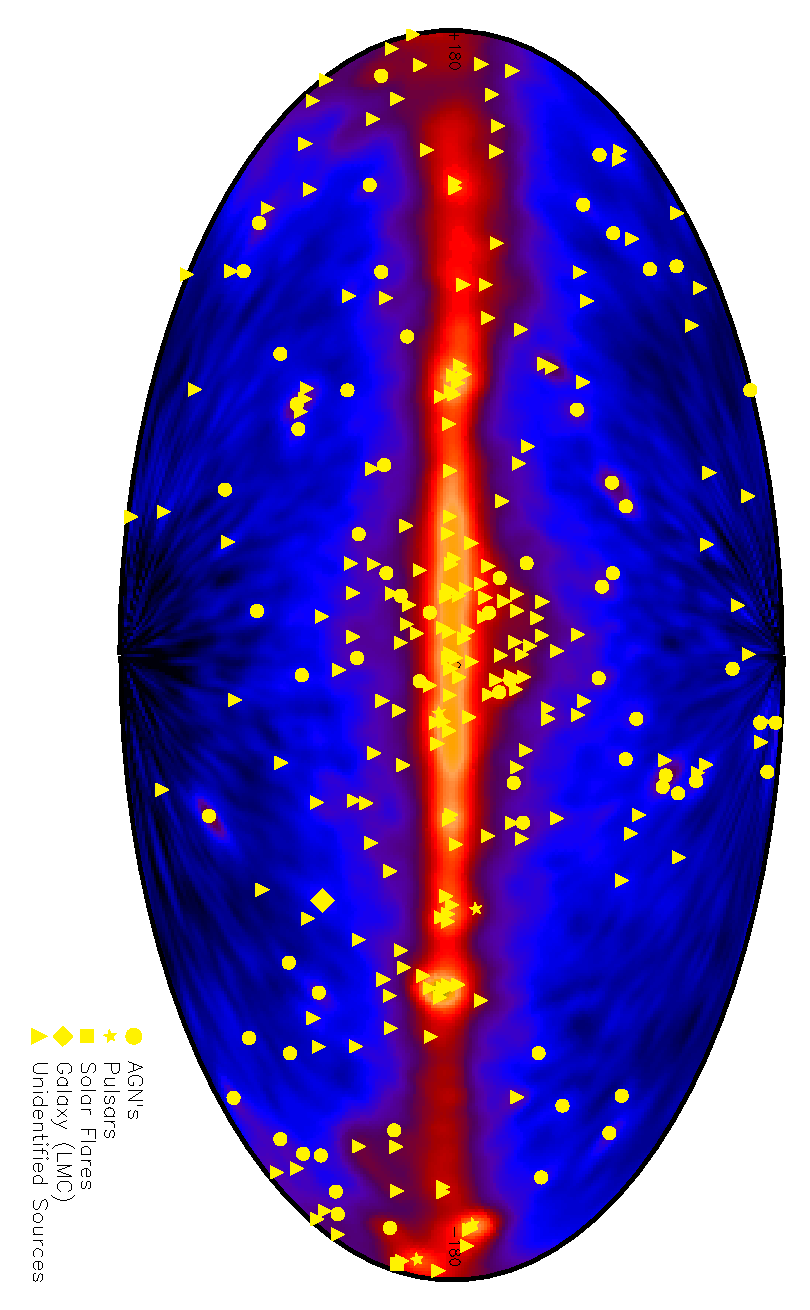
\includegraphics[width=0.8\columnwidth,angle=90]{Figures/3rd_egret_cat.eps} }
	\caption[Third EGRET catalog all-sky map.]{Third EGRET catalog all-sky map. Unidentified sources represented by triangles. Image courtesy of \url{https://heasarc.gsfc.nasa.gov/docs/cgro/images/epo/gallery/skymaps/}}
	\label{fig:3EGSky} 
\end{figure}

In spite of the difficulties in \egret{} source association, many studies have attempted correlating the unidentified \egret{} sources with various Galactic populations. In particular, several authors found strong evidence for statistical correlation between \glspl{snr} and some of the low-latitude unidentified sources \citep{Sturner95, Esposito96, Romero99}. In a review of the state of potential \snr{} /  \egret{} associations, \cite{Torres03} showed that there were 19 unidentified \egret{} sources that had an \snr~fall within its 95\% error box. Performing Monte Carlo simulations of the population of  \egret~sources, they determined that the chance probability for the 19 sources to be coincident with an \snr~was $1.05 \times 10^{-5}$, implying a probability of 0.99998 that at least one of the associations is real. Despite the statistical correlation of \egret~sources with \glspl{snr}, there were no definitive associations of an \snr~with any \egret~sources.

As the successor to \egret{}, the \lat{} was designed to improve upon its predecessor in a multitude of areas relevant to detecting \snrs{} \citep{atwood09,lat_perf}. The \lat{} has a much improved angular resolution (68\% single-photon containment radius $\sim 0.4^{\circ}$ at 1\gev{} for photons with the best quality direction reconstruction, PSF3 event type, compared to $\sim 1.7^{\circ}$ for \egret{} at the same energy), necessary to resolve \snrs{} as extended objects. The \lat{} also benefits from a superior sensitivity due to a combination of the improved \psf, larger peak effective area ($ {\rm > 9000~cm^2}$ vs. ${\rm \sim 1500~cm^2}$), wider \fov{} (2.4 sr, which is nearly 5 times that of \egret{}), and deeper, more-uniform sky exposure (afforded by the \lat's scanning observations as opposed to \egret's pointing operation). 

This bump in sensitivity results in the \lat{} detecting considerably more sources than \egret. Remarkably, within its first three months of commission, the \lat{} detected 205 sources above {\rm 10$\sigma$ significance \citep{lat_3m}, and by 11 months, 1451 sources above 4$\sigma$ \citep{1FGL}, compared to  the aforementioned 271 over the entire \egret{} mission. In fact, over its lifetime, \egret{} detected a total of about ${\rm 1.5~x~10^6}$ cosmic photons \citep{Thomson93}, while as of March 2016, the \lat{} has detected ${\rm \sim 863~x~10^6}$ \jamie{change this number in June} source class photons. The \lat's point-source sensitivity peaks between 1 and 10\gev{}, depending on location on the sky. With its increased sensitivity and higher energy range (up to $\sim$ 2\tev{} with the recent Pass 8 event reconstruction improvements, which is nearly an order of magnitude higher than \egret{}), the \lat{} is uniquely situated to study the \gam{} morphology and spectra of \snrs{}.
	
Both energetic lepton interactions (\ie \ic{} radiation of relativistic electrons interacting with ambient photon fields, and nonthermal \brems{}) and hadronic processes ($\pi_0$ decay \gam{}s from \cray{} protons encountering surrounding nuclei) produce spectra observable at \gam{} energies (see Chapter \ref{chap:gamAstr} for details). While the \ic{} generating electron population is also observable through emission of radio \sync{} photons, the proton-proton interaction solely emits \gam{}s. Despite being the prime energy range to observe the effects of cosmic particle acceleration, complexities at the lower \lat{} energy range stymie \snr{} morphology studies.
	
The \lat{} detects a strong, soft band of diffuse emission in the Galactic plane due to the interactions of  \crs{} with interstellar material. This bright diffuse radiation combined with the multiple potential emission scenarios, broadening \psf{} at decreasing energy, and a high source density in the plane can make it difficult to spatially disentangle sources observed by the \lat{}. To circumvent these 
difficulties, the majority of the analyses undertaken in this thesis are focused on the ${\rm E \geq 1\gev}$ energy range. This energy band is ideal for probing the properties of the accelerated particle populations present in the \snr{} environment. Studies of  \snrs{}  above 1\gev{} benefit from finer \lat{} \psf{}, striking a balance between minimizing the diffuse contribution, maximizing photon sensitivity, and retaining good photon statistics. Furthermore, evolved \snrs{}  exhibit a spectral break between 1-10\gev{} \citep{Hewitt15}. Explanations for the break range from Alfv\' en wave evanescence generated by collisions of partially ionized material in \mcs{} overtaken by \snr{}  shocks \citep{Malkov11}, reflected shocks in clouds \cite{Inoue10c}, and energy-dependent diffusion from shocks \cite{Ohira11}. Studying \snrs{} in this energy range hones our capability to tackle several goals set out by the \Fermi{} team when the mission was conceived.

\snr{I need to end with something about how/why awesome \Fermi{} has and will continue to be in searching for SNRs?mmaybe}
\section{Summary}\label{Rems:summ} In this section we summarized the end phase of stellar evolution (just enough to motivate SNRs) and descried the environs surrounding the supernova; development and phases of \glspl{snr} (and \glspl{pwn}?).  In particular we detailed the nonthermal emission mechanisms that produce \g-ray radiation, detection of young vs middle-aged( evolved, interacting with surroundings/dense medium),TeV detects younger typically, the troubles of detecting extension from them(?) something about different emission zones? Troubles disentangling hadronic from leptonic at \g-rays. \g-ray spectral and morphological features. Trends across the population wrt spectral shape/breaks, higher luminosity for interacting rems. Cosmic rays, using gamma-rays to probe CR population. So much of \g-ray astro is really about studying CRs, how much to say about them? 

\section{Scratch}
This chapter needs a different title. It's more focused on the specific sources being studied in this thesis. Galactic extended sources, SNRs, PWNe, but as in the SNRcat, not just extended SNRs, point-like SNRs as well.

Less focus on PWNe. Only give as much as I feel I need to support mentioning them a bit for 2FHL?

The focus of this section is supernova remnants in a gamma-ray context. Theory of evolution, what the gamma-ray emission is like, what we can learn from them individually.  This leads to the 1st SNR cat section for what we can do with them ensemble

NOt sure I really need any PWN stuff yet

in 2FHL we detect some pwn. If including above 10gev work, they'll be there too. Much of the thesis is really about extended gamma-ray sources, but not sure how that fits into the title and chapters yet

Do I need to get into composite SNRs (composite means SNR + PWN ) Maybe relevant for G150? Some things about interaction of reverse shock with PWN and crushing/reverberations of the PWN?

\cite{Montmerle79}
\chapter{Gamma-ray Astronomy}
\label{chap:gamAstr}

The story of \gam 's from astrophysical objects is a tale of the most extreme, energetic, and violent environments in our universe. Discovered by Paul Villard studying radiation from radium and named by Ernest Rutherford, who previously uncovered the nature of $\alpha$ and $\beta$ radiation, 

accelerator plus target often {}
gamma-rays, gamma-ray astronomy, gamma-ray sky, connection to CR

gamma-ray production mechanisms

gamma-ray astronomy is really a proxy for studying cosmic rays and acceleration/diffusion processes. How much to get into CR. 

gamma-ray telescopes leads into the LAT, Egret was  predecessor , what it did and what were some relevant unanswered questions regarding supernova remnants 
    
Maybe combine the telescope stuff  with the LAT section and leave this section for history and astrophysics of \g-rays? Or just combine this section with  LAT section?

Altho' many miles from bomb zero, Dr. Bruce Banner is bathed in the full force of the mysterious Gamma Rays!
\chapter{The \Fermi{ }Gamma-Ray Space Telescope and \gam{} Data Analysis}
\label{chap:FGST}

\begin{figure}[ht!]
	\centering
	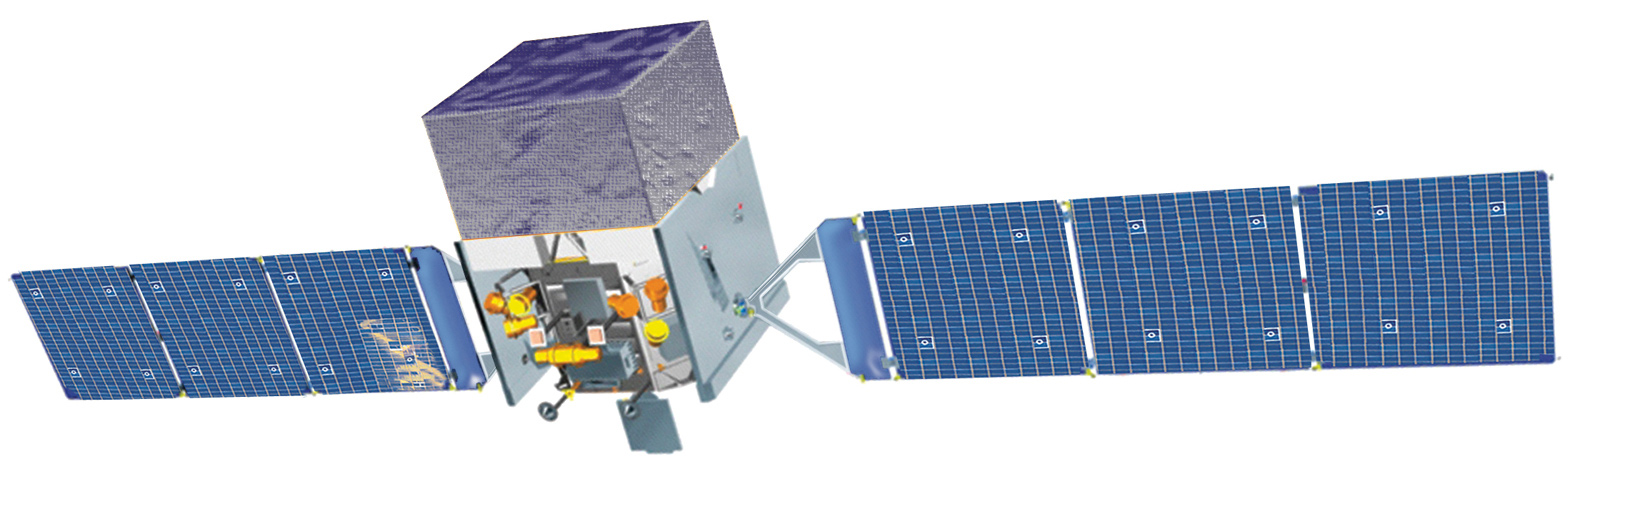
\includegraphics[width=1.0\columnwidth]{Figures/Fermi_telescope_illustration_01.jpg}
	%\caption[Fermi ]{Fermi}
	\label{fig:fermi}
\end{figure}

\section{\label{FGST:intro}Introduction}
The \Fermi{} Gamma-Ray Space Telescope (\Fermi{} ~hereafter), successor to the \egret{} instrument on the \cgro{}, was successfully launched into orbit around Earth on June, 11 2008. \Fermi{} consists of two instruments, the \lat{} and the \gbm{}. The \lat{}, which is the primary instrument on \Fermi{}, is a pair conversion telescope designed to detect photons from 20\mev{} to greater than 1\tev{} \citep{atwood09, lat_perf, 2FHL} Its standard mode of operation is a sky-survey mode in which it observes the entire sky every 3 hours. The secondary instrument aboard \Fermi{}, the \gbm{}, was designed to detect \gam{} bursts in a waveband overlapping that of the \lat{} yet complementary in that its energy extends considerably lower. Combined the \lat{} and \gbm{} comprise a formidable observatory, spanning more than 8 decades in energy, and it is currently the only instrument performing all-sky observation in this broad energy range. 

\begin{figure*}[!]
	\begin{center}
		\hspace*{-1.5cm} \begin{tabular}{ll}
			\includegraphics[width=6.5cm]{Figures/{231388main_fairopen-lg_full}.jpg} &
			\includegraphics[width=6.5cm]{Figures/{glast_readytogo}.jpg} \\
			
			\includegraphics[width=6.5cm]{Figures/{seth_02}.jpg} &
			\includegraphics[width=6.5cm]{Figures/{seth_2356}.jpg} \\

		\end{tabular}
	\end{center}
	\caption[\Fermi{} launch images.]{
		\label{fig:Launch}{Top left: \Fermi{} being loaded on to a Delta II 7920-H rocket after arriving at Cape Canaveral. Top right: Delta II rocket  at Space Launch Complex 17B with \Fermi{} on board. Lower Left: Dr. Elizabeth Hays at Cape Canaveral marveling at the majestic launch of the \Fermi{} observatory. Lower right:.\Fermi{} was launched into a 550 km, low Earth orbit, on June 11 2008, at 16:05 UTC. Images courtesy of NASA and Seth Diegel.}
	}
\end{figure*}

\section{\label{FGST:LAT}The Large Area Telescope}
Due the nature of interaction between \gam{}s and matter, photons of \gam{} energies cannot be reflected or refracted in the same way as lower energy light can be, which restricts the design possibilities of a \gam{} telescope. Because of this limitation, \Fermi{} uses the photon pair-production phenomenon to detect \gam{} photons. Photon pair production refers to the mechanism by which a
photon with sufficient energy (at least twice the rest mass of an electron) can convert to an electron/positron pair. The conversion from photon to antimatter pair can occur in the presence of a nucleus whose Coulomb field can absorb and thus conserve the momentum of the photon. Figure \ref{fig:pairProd} top shows the probability of photon conversion for given energies, demonstrating how higher atomic-number (and thus stronger field) nuclei, are more conducive to conversion by providing a larger interaction cross section. Figure \ref{fig:pairProd} bottom plots the interaction cross section versus photon energy. Above 10 \mev{}, photon pair production (${\rm \kappa_{nuc}}$) is the clearly dominant photon interaction process \citep{Beringer12}.

\begin{figure}[!]
	\centering
	\vspace{-0.5cm}
		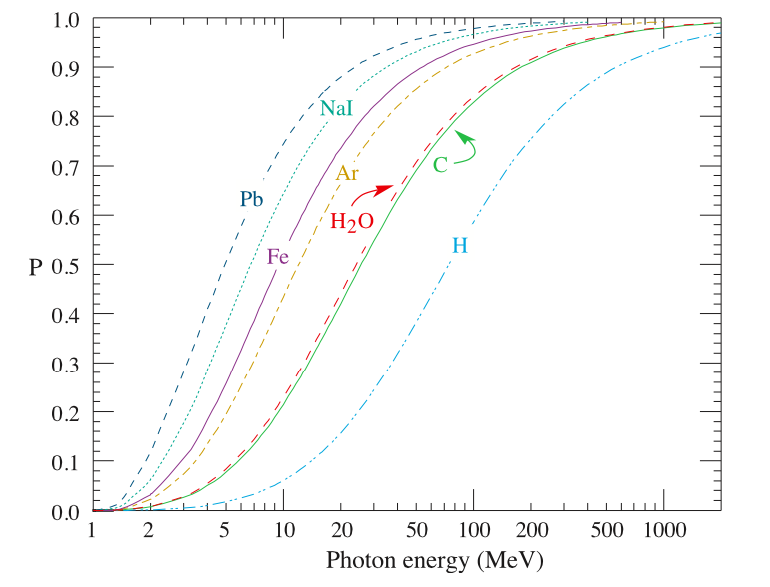
\includegraphics[width=0.85\columnwidth]{Figures/Beringer12_30_17.png}
		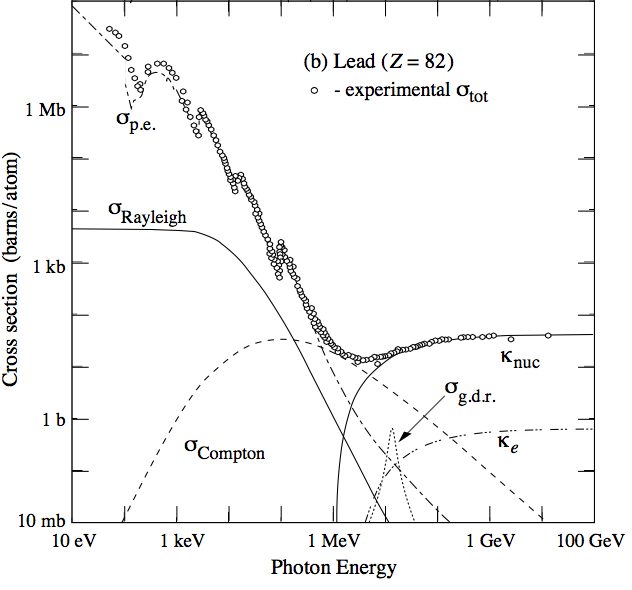
\includegraphics[width=0.85\columnwidth]{Figures/Beringer12_30_15.png}
	\caption[Top: Probability of photon conversion to e$^-$ e$^+$ pair. Bottom: Photon cross section versus energy]{Top: Probability that a photon interacting with various nuclei will result in an \ee{} pair as a function of energy. Bottom: Photon cross section versus energy for various photon-matter interaction channels. Both figures originally from \cite{Beringer12} as Figure 30.17 and 30.15.}
	\label{fig:pairProd}
\end{figure}

The \lat{} instrument on board \Fermi{} is composed of three subsystems, all designed to take advantage of the pair production mechanism. First and foremost, is the \tkr{}. The \lat{}'s \tkr{} is a module consisting of 18 x-y paired silicon strip detectors that measure the trajectories of the pair-produced charged particles. The silicon strips are interleaved with a tungsten foil to promote \gam{}s passing through the material to convert to \ee{} pairs. The \lat{} is made up of 16 towers (arranged in a 4x4 grid), with each tower containing the 18 interlaced silicon, tungsten planes. The top 12 layers of the \tkr{} comprise the "front section" and are made of 3\% radiation length tungsten. The next 4 layers constitute the "back section" of the \tkr{} and are made of thicker, 18\% radiation length tungsten foil. The final two \tkr{} layers contain no tungsten and are present as a requirement of the \tkr{} trigger which requires at least three hits in adjacent layers to trigger \citep{lat_perf}. The front section of the \tkr{} was designed to minimize the separation between tungsten and silicon (\ie{}\ the point of conversion and subsequent detection) minimizing multiple scattering effects therein, and thus optimizing the \psf{} for events converted in this section. The 6-times-thicker back layers were designed to further promote conversion, maximizing the effective area of the \lat{}, yet sacrificing resolution for events converting in this layer.
% Figure \ref{fig:Tower}, shows a diagram of a single tower with \tkr{} components included.

The next subsystem of the \lat{} is the \calo{}. The \calo{} (located at the bottom of each of the 16 towers) is comprised of 96 CsI scintillation crystals, arranged in 8 layers of 12 logs. This construction allows the \calo{} to {\bf 1.} measure the energy deposition of the shower of particles resulting from the incident photon's pair-produced \ee{} pair, and {\bf 2.} to perform 3D imaging of the shower, which can serve as a measurement of shower energy leakage.

%\begin{figure}[h!t]
%	\centering
%	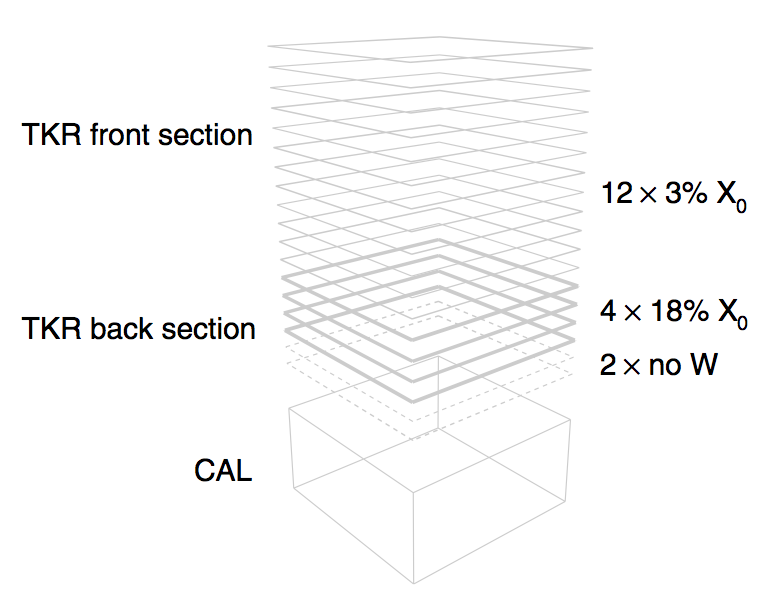
\includegraphics[width=1.0\columnwidth]{Figures/latPerf_Tower.png}
%	\caption[LAT tower schematic ]{\lat{} tower schematic showing the different \tkr{}layers and ending with the \calo{} on the bottom of the tower. Taken from \cite{lat_perf}}
%	\label{fig:Tower}
%\end{figure}

The final vital component of the \lat{} is the \acd{}. The role of the \acd{} is to reject background charged particles that enter the \lat{} to avoid misclassifying them as photons. The design of the \acd{} was informed by lessons learned from the \lat{}'s predecessor, the \egret{} instrument on \cgro{} \citep{Mosieev05}. In the \calo{} the electromagnetic shower generated by the incident photon produces secondary particles as well as X-rays. These X-rays can Compton scatter the charged particles out through the 
\tkr{} and \acd{} (referred to as ``backsplash'') creating false vetoes. This backsplash was present in \egret{} and reduced the efficiency of the instrument above 10 GeV \cite{atwood09}. To overcome the backsplash effect, the \lat{} uses a segmented rather than monolithic layer for the \acd{}, made up of 89 scintillating tiles surrounding the towers (as in Figure \ref{fig:latGuts}).

\begin{figure}[ht!]
	\centering
	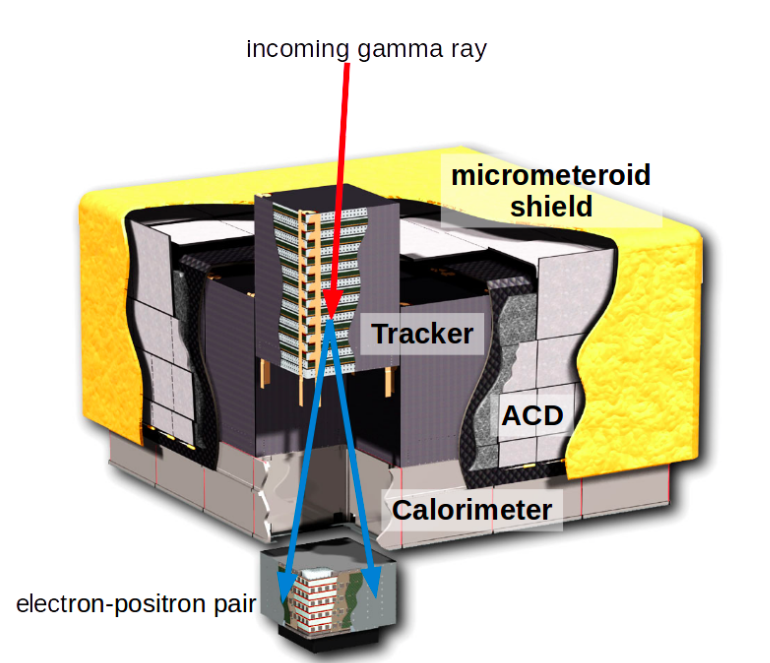
\includegraphics[width=1.0\columnwidth]{Figures/latGuts.png}
	\caption[Diagram of the three primary LAT subsystems]{Diagram of the \lat{} subsystems demonstrating how an incident \gam{} can enter through the top layer of the \acd{}, convert to a \ee{} pair in a layer of the \tkr{}, and finally deposit its energy in the \calo{}.}
	\label{fig:latGuts}
\end{figure}
 
\section{\label{FGST:perf}LAT Performance}
The \lat{} performance is dictated by the telescopes hardware and software designs (\eg{}\  event reconstruction methods, background and event classifications). The parameterizations of the performance are referred to as the \irf{}. The \lat{} \irf{} are factorized into three terms:
\begin{enumerate}
	\item {\bfseries \psf{}, P${\mathbf{(\hat{v^\prime};E,\hat{v})}}$:} Represents the angular resolution of the \lat{}. It is the probability density for reconstructing an incident \gam{} with position $\hat{v^\prime}$ if the true position is $\hat{v}$ for given energy E. The \psf{} is strongly energy dependent. At low energies, this dependence is dominated by multiple scattering in the \tkr{} causing the \psf{} to broaden, and at higher energies (above a few \gev{}) it is dominated by the strip pitch, or the distance between adjacent silicon strip centers, which limits how fine the \psf{} can be at high energies.
	
	\begin{figure*}[ht]
		\begin{center}
			\includegraphics[width=1.\columnwidth]{Figures/{gPsfAve95Energy_P8R2_SOURCE_V6fb_10MeV}.png}
		\end{center}
		\caption[LAT P8R2\_SOURCE\_V6 angular resolution.]{
			\label{fig:PSF}{\lat{} angular resolution for 68\% and 95\% containment radius and front and back converting events as a function of energy for the P8R2\_SOURCE\_V6 event classification. Figure from \url{https://www.slac.stanford.edu/exp/glast/groups/canda/lat_Performance.htm}}}
	\end{figure*}
	
	\item {\bfseries Effective Area, A${\mathbf{ _{eff}(E,\hat{v})}}$}: Represents the collecting area of the \lat{}. It is the product of the geometric cross section of the \lat{} and a dimensionless term that quantifies the efficiency for detecting and reconstructing gamma rays that pass into the detector volume. It has units of area. 
	
	\begin{figure*}[ht]
			\begin{center}
				\includegraphics[width=1.\columnwidth]{Figures/{gAeffEnergy_P8R2_SOURCE_V6fb_10MeV}.png}
			\end{center}
			\caption[LAT P8R2\_SOURCE\_V6 effective area]{
				\label{fig:Aeff}{\lat{} effective area for front, back, and total converting events as a function of energy for the P8R2\_SOURCE\_V6 event classification. Figure from \url{https://www.slac.stanford.edu/exp/glast/groups/canda/lat_Performance.htm}.}}
	\end{figure*}
	
	\item {\bfseries Energy Dispersion, D${\mathbf{(\hat{E^\prime};E,\hat{v})}}$}: Represents the energy resolution of the \lat{}. It is the probability density for reconstructing an incident \gam{} with energy $\hat{E^\prime}$ if the true energy is $\hat{E}$ for given direction on the sky. Energy dispersion effects are often ignored in \lat{} analysis above a few hundred \mev{} as \cite{lat_perf} showed that the effects of neglecting it are of the order of a few percent.
	
		\begin{figure*}[ht]
			\begin{center}
				\includegraphics[width=1.\columnwidth]{Figures/{gEdispAve68Energy_P8R2_SOURCE_V6fb_sep_10MeV}.png}
			\end{center}
			\caption[LAT P8R2\_SOURCE\_V6 energy resolution]{
				\label{fig:Edisp}{\lat{} energy resolution for front, back, and total converting events as a function of energy for the P8R2\_SOURCE\_V6 event classification. Figure from \url{https://www.slac.stanford.edu/exp/glast/groups/canda/lat_Performance.htm}.}}
		\end{figure*}
	
\end{enumerate}

In general, the \lat{} has a large effective area (${\rm \sim 9500 cm^2}$ at a few \gev{}) (Figure \ref{fig:Aeff}), energy resolution of 5\% (at 10 \gev{}) to 20\% (at 100 \mev{}) (Figure \ref{fig:Edisp}), and a single-photon angular resolution ranging from $\sim 3.2^\circ$ at 100 \mev{} to $
\lesssim 0.16^\circ$ for E $>$ 10 \gev{} (Figure \ref{fig:PSF}). With its rocking mode observation strategy (35$^\circ$ north of the zenith axis for one orbit, and then south for the next) and its  wide \fov{} of 2.4 sr, the \lat{} attains a nearly uniform coverage of the sky within two orbits, or 3 hours. The culmination of the \lat{}'s performance can be summed up as its capability to detect distinct sources on the sky. Figures \ref{fig:sensMap} and \ref{fig:sensSlice} depict the \lat{}'s threshold for detecting emission from a point source above the structured Galactic diffuse emission (described in Chapters \ref{gamAstr:Emiss} and \ref{FGST:bkg}). Figure \ref{fig:sensMap} demonstrates what level of emission the \lat{} can detect when integrating over the majority of its energy range, and Figure \ref{fig:sensSlice} shows what the  source detection threshold is for detecting sources in individual energy bins and at four locations on the sky. See \ref{Rems:latGam} for a comparison of the \lat{}'s capabilities with that of \egret{}.

\begin{figure*}[!ht]
	%\begin{centering}
	\hspace{-2.7cm}
	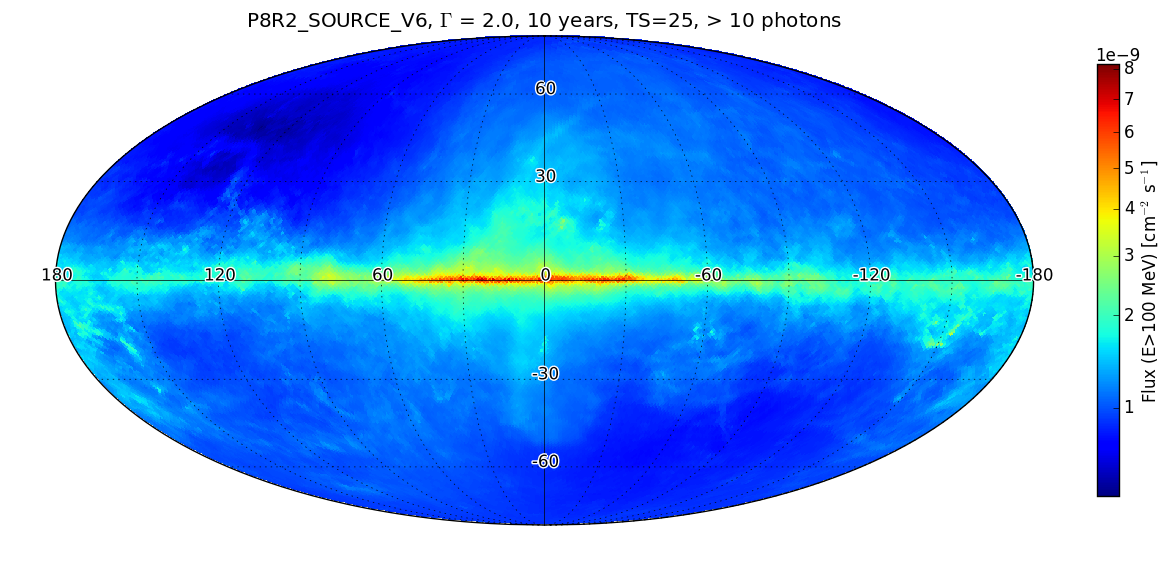
\includegraphics[width=1.3\columnwidth]{Figures/allsky_flux_sensitivity_p8r2_source_v6_all_10yr_zmax100_powerlaw_g200_n10_ts25.png}
	\caption[LAT simulated,  10 year, P8R2\_SOURCE\_V6 integral-flux sensitivity map]{\lat{} simulated, 10 year, integral-flux sensitivity map for P8R2\_SOURCE\_V6 event classification. The all-sky map was created for energies above 100\mev{} and for a point source (modeled as a \pl{} of spectral index 2) to obtain a $5\sigma$ significance. Figure from \url{https://www.slac.stanford.edu/exp/glast/groups/canda/lat_Performance.htm}.
		\label{fig:sensMap}}
	%\end{centering}
\end{figure*}

\begin{figure*}[!ht]
	\begin{centering}
		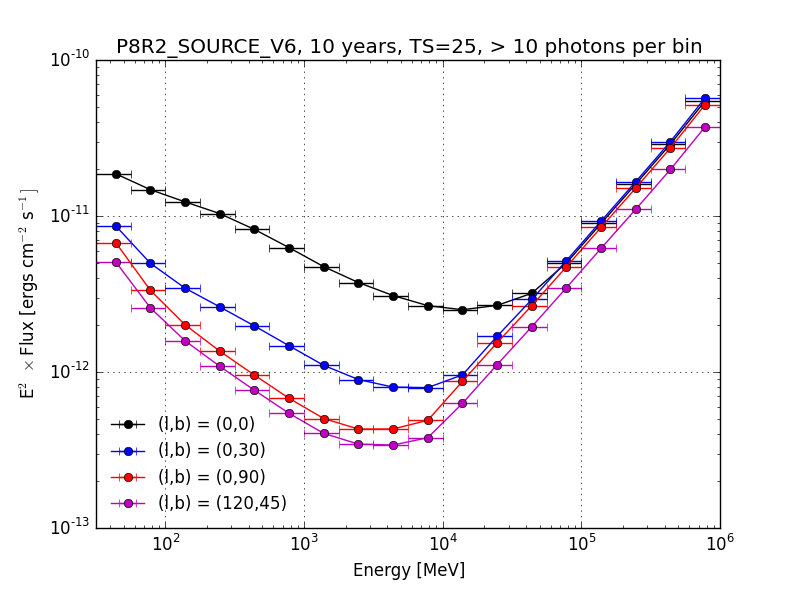
\includegraphics[width=1.0\columnwidth]{{Figures/differential_flux_sensitivity_p8r2_source_v6_all_10yr_zmax100_n10.0_e1.50_ts25}.png}
		\caption[LAT 10 year, P8R2\_SOURCE\_V6 differential-flux sensitivity for four locations on the sky.]{\lat{} 10 year, differential-flux sensitivity map for P8R2\_SOURCE\_V6 event classification. The all-sky map was created for energies above 100 \mev{} and for a point source (modeled as a \pl{} of spectral index 2) to obtain a $5\sigma$ significance. Figure from \url{https://www.slac.stanford.edu/exp/glast/groups/canda/lat_Performance.htm}.
			\label{fig:sensSlice}}
	\end{centering}
\end{figure*}

For a given \gam{} source model $S(E,\hat{p})$ (where the source model refers to either point sources, extended sources, or background Galactic diffuse or isotropic emissions), \ie{}\ the number of photons per unit time, energy, and solid angle at a given time, energy, and position on the sky, where $\hat{p}$ is the direction on the sky, we can convolve the source model (times the effective area) with the dispersion components (\psf{} and  energy dispersion) to obtain the predicted differential source counts (in counts per unit energy/time/solid angle) by integrating over the energy and time range of interest and over the solid angle in the \lat{} reference frame:
\begin{align}\label{eq:exCountsPred}
	M(E^{\,\prime},\hat{p}^{\,\prime}) =  \int \int \int S(E,\hat{p}) A _{eff}(E,\hat{v}) \times \nonumber \\
	P(\hat{v}'(t,\hat{p}^{\,\prime}); E, \hat{v}(t;\hat{p})) D(E^{\,\prime}; E, \hat{v}(t;\hat{p})) dE d\Omega dt.
\end{align}

All the values discussed above are particular to the recent \lat{} event-level reconstruction update colloquially referred to as Pass 8 \citep{atwood13}. Pass 8 consists of a series of improvements to the \lat{}'s event selection process. The three primary areas of improvement are in the event reconstruction methods, background rejection, and Monte Carlo simulations of the detector using flight data. One improvement example involves the way in which the  \lat{} reconstructs and tracks the path of an \ee{} pair back to an incident photon. Previously a track-by-track pattern recognition algorithm was used to find the two antimatter paths and combine them back to determine the vertex of conversion. The improved method uses a tree-based tracking method that considers conversion in the \tkr{} as the start of an electromagnetic shower and attempts to model this process by grouping hits in the \tkr{} into one or more ``trees". Similar event reconstruction methods have also been applied to the \acd{} and \calo{}. 

The combined effects of the various upgrades result in an extension of the energy down to 30\mev{} and up to 3\tev{} \cite[see Chapter \ref{chap:2FHL} for applications]{Bruel12}, a 40\% gain in point-source sensitivity, up to a 2$\times$ increase in acceptance (defined as effective area integrated over solid angle) below 100\mev{} and above 100\gev{}, and a narrower \psf{} at high energies. Several new event classifications have also been developed (in addition to the previous front and back event types) to leverage the newfound  Pass 8 \lat{} capabilities. Specifically, there are new event types that define the quality of event reconstruction for both the \psf{} and energy dispersion, by partitioning events into quartiles based on quality, allowing for an even finer grade energy and spatial resolution.

%\begin{equation}\label{eq:exposureDef}
%\mathcal{E}(E,\hat{p},s) = \int  A _{eff}(E,\hat{v}) dt.
%\end{equation}

%\begin{equation}\label{eq:tobsDef}
%\mathcal{E}(E,\hat{p},s) = \int  A _{eff}(E,\hat{v}) t_{obs}(\hat{v};\hat{p}) d\Omega.
%\end{equation}


\section{\label{FGST:analysis}\FermiLat{} Data Analysis Method}
The standard method for analyzing astrophysical data at other wavelengths (\eg{}\ optical) is by performing aperture photometry. This consists of essentially counting the photons ``on-source'' in a extraction region, estimating background ``off-source'' in a neighboring region, where the background is typically assumed to be isotropic, and including that background in the model of the region. Although not always simple, various source quantities can typically be derived from the data itself (\eg{}\ intensity, extent if resolvable). The aperture photometry method is not feasible for analysis of \Fermi{} data (as was the case for \egret{} \cite{mattox96}) due to various complexities inherent to detecting \gam{} photons. 

The first such issue is that because of the breadth of the \lat{} \psf{}, and wide energy range of the \lat{}, source confusion abounds and sources are not truly isolated from one another. The overlapping tails of the \psf{} would make analysis via aperture photometry particularly intractable at low energies (where the \psf{} rises steeply with decreasing energy, see Figure \ref{fig:PSF}) and in the Galactic plane (with a high source density and strongly anisotropic diffuse emission).\jamie{\ref{FGST:diff?}} The second reason is the complex relationship between an individual source and the \irf{}. Since \Fermi{} typically operates in a sky-survey mode, photons from an individual source need to accumulate over long integration times, and the orientation of the space craft with respect to the source of interest will vacillate over time. The response of the telescope is dependent on the orientation of the space craft, so it is non-trivial to determine source and background fluxes by simply counting photons.

To circumvent the issues described above, \cite{Cash79} applied the maximum likelihood method to astrophysical counting-experiments and parameter estimation of X-ray data. \cite{mattox96} then established a framework for analyzing \egret{} \gam{} via the maximum likelihood method. The likelihood, \like{}, is defined as the probability of obtaining the data observed assuming a model of the sky. In the maximum likelihood framework, we want to estimate the model parameters by maximizing the likelihood and finding the  parameters that best-fit the data. Since the \lat{} is a particle detector, and hence a photon counting experiment, the observed counts are distributed as a Poisson distribution with unknown mean. For large data sets it is more tractable to use a binned maximum likelihood analysis; binning in both position on the sky and energy. The binned maximum likelihood function for \lat{} is thus given as:
\begin{equation}\label{eq:posLike}
{\rm \like{} = \prod_{i} \frac{m_i^{n_j}e^{-m^i}}{n_i!}}
\end{equation}
Thus the likelihood is the product of the Poisson probabilities over all j positions and energies, where ${\rm m_i}$ is the expected counts in the i\textsuperscript{th} bin, and ${\rm n_i}$ is the observed counts in the i\textsuperscript{th} bin.  It is often computationally easier to work with the log of the likelihood, so taking the log of \ref{eq:posLike} gives:

\begin{equation}\label{eq:like}
{\rm \logL{} = -\sum_{i} m_i + \sum_{i} n_j~log~m_j}
\end{equation}
where we have dropped the arbitrary constant  ${\rm -log~n_i!}$. The term $\sum_{i} m_j $ is the total expected counts in all bins. The model counts ${\rm m_i}$ are calculated by integrating the differential source model (given by \ref{eq:exCountsPred}) over the i\textsuperscript{th} bin for all sources. The \Fermi{} Science Tools were designed to perform the tasks involved in binning the sky in position and energy, calculating the convolution integral in \ref{eq:exCountsPred}, and computing the likelihood of \ref{eq:like} (implemented via {\tt gtbin, gtsrcmaps, and gtlike} respectively).

The other way in which \Fermi{} employs the maximum likelihood method is through the \lrt{} to assess detection source significance and compare model hypotheses. The \lrt{} is a statistical method to assess the goodness-of-fit of two different models. The likelihood is calculated for two models, one of which can be reduced to the other hypothesis under certain conditions. If the more complex model can be reduced to the simpler model (called the null hypothesis), we say the simpler hypothesis is nested within the more complex. In the \lrt{}, the \ts{} is defined as: 

\begin{equation}\label{eq:LRT}
\rm \ts{} \equiv 2\log(\like{}(H_1)~/ \like{}(H_0)),
\end{equation}
with ${\rm H_1}$ being the more complex hypothesis and ${\rm H_0}$ the null. \cite{mattox96} detail how by Wilks' theorem, the \ts{} for detection of a point source (with the null hypothesis being that with no source present, or 0 flux) will be asymptotically distributed as a chi-squared distribution in the null hypothesis in the limit of a large sample size, N. For photon counting experiments, N is the number of events relevant to the parameter being estimated, and the expected deviation of the \ts{} from the chi-squared distribution is of order ${\rm N^{-1/2}}$ \cite{Cash79}. Specifically,


\begin{equation}\label{eq:tsPdf}
\rm PDF(\ts{}) = 1/2~\chi^2_1,
\end{equation} 
where PDF(TS) is the probability distribution function for obtaining a specific value of \ts{} and $\chi^2_1$ is the chi-squared  distribution for one degrees of freedom.   The factor of 1/2 arises from the fact that the flux of a source is not permitted to be zero, and since negative and positive fluctuations in a parameter's value contribute equally to the \ts{}, half of the distribution is lost with the positive flux restriction. The significance of detection is oft quoted as ${\rm \sigma \approx \sqrt{TS}}$, which is strictly valid only for $\chi^2_1$. More generally, when comparing the likelihood of two models with n degrees of freedom between them, equation \ref{eq:tsPdf} applies, but using  $\chi^2_n$ for n degrees of freedom versus one.

\section{\label{FGST:bkg}Modeling Diffuse Background Emission}
As discussed in Chapter \ref{gamAstr:Sources}, to characterize point-like or spatially extended  \lat{} sources, it is necessary to have an accurate model of the Galactic diffuse background emission. The standard model for the Galactic radiation adopted for \lat{} analysis \citep{diffuse16} is derived from a linear combination of gas column density maps (HI and CO) and infrared dust emission maps to trace the interstellar gas for a given \gam{} energy range. The templates describe the \gam{} photon intensity resulting from \crs{} interacting with the gas through \brems{} and neutral pion decay processes. Another component of the templates is derived from the cosmic ray propagation code, {\tt GALPROP} \citep{strong98,strong07}, which calculates the \gam{} intensity of \crs{} \ic{} scattering ambient, interstellar photons. The model assumes a uniform \cray{} density in each template, so to accommodate for possible radial variations in the \cray{} density, the templates are divided into 9 Galactocentric annuli. 

A second, nearly-isotropic, background component is also accounted for in typical \lat{} analyses. The isotropic emission observed by the \lat{} consists of charged particles entering the \lat{} that are misclassified as \gam{}s as well as \gam{}s from unresolved, sub-threshold sources observed across the sky \citep{isoSpec}.

Both the Galactic and isotropic backgrounds are factored into the likelihood analysis framework, described in Chapter \ref{FGST:perf}, and in particular by Equation \ref{eq:exCountsPred}. The Galactic diffuse emission is included via the aforementioned spatial and spectral templates which are typically modulated by a power-law function (to account for deviations in intensity from the template at each energy) with a normalization and spectral slope that are free to vary in the likelihood analysis. The isotropic component is simply scaled by a normalization parameter, also typically free to vary.

%The model of the sky will contain terms describing the sources (\ie{} the flux density of all the sources in the region, or $S(E,\hat{p})$ in \ref{FGST:LAT}), the background`


%\chapter{Analysis of \lat- data}
\label{chap:fermiData}
I'm not sure about this chapter yet. Maybe it's a general section on Analysis of Fermi data, why maximum likelihood, how it's formulated,  implemented in the Science Tools, pointlike and the analysis for extended sources. Diffuse emission

Four steps to going from observing the sky to final LAT analysis:

Instrument taking data: How we get to counts

Reconstruction : How we get photons

Likelihood: How to characterize sky using response functions, point source  and diffuse modeling

Likelihood for ES: how to use likelihood methods to char and resolve sources measure  extension


\section{addSrcs}

 %merged with LAT section
\chapter{An Automated Method for LAT Analysis of the Galactic Supernova Remnant Population}
\label{chap:snrcat}


\section{Introduction}\label{snrCat:Intro}
Two of the primary science goals of the \lat{}  are to 1. resolve the \gam~sky, uncovering the nature of the unidentified sources detected by \egret{}, and 2. to understand the mechanisms of cosmic particle acceleration \citep{atwood09}. In this chapter, we describe our efforts towards addressing these questions by studying the \gam{} emission coincident with sources comprising the population of known radio emitting \snrs{}.

Prior to this work, several individual studies with the \lat{} had successfully resolved spatially extended emission from \snrs{} \citep[and references therein]{2FGL}, yet no systematic analysis leveraging the \lat{}'s full-sky coverage had thus been attempted. We performed for the first time a uniform study of the \snrs{} in aggregate to measure the properties common to these objects. An understanding of these common characteristics allows us to assess \snrs{} as a class of \gam{} and \cray{} emitting objects and serves as the impetus for this uniform analysis of the known Galactic \snrs{}. We report here on the published results from the \snrcat{} \citep{snrCat}.
 

%%%%%%%%%%%%%%%%%%%%%%
%%%%%%%%%%%%%%%%%%%%%%

\section{\label{snrcat:ptlk}The \ptlike{} Maximum-Likelihood Package and \srcs{}}

As described in Chapter \ref{FGST:analysis}, maximum-likelihood analysis is the ideal method for determining the properties of \lat{}-observed sources due to the ``counting-experiment" nature of \FermiLat{}. The standard maximum-likelihood tools for analyzing \lat{} data are implemented via the \Fermi{} Science Tools, and in particular \gtlike{}.  Despite being the optimum method, likelihood analysis of \lat{} data is complex due to the highly non-linear performance of the instrument and can be computationally expensive. It is necessary to manage the data and response of the telescope as well as the source and background models. Furthermore, due to the broadening of the \psf{} at low energies, even when studying a single source, it is necessary to include in the model descriptions of multiple surrounding sources. The \ptlike{} binned maximum likelihood package was created to ameliorate some of these issues. Described in detail in \cite{Kerr10}, \ptlike{} is an alternate likelihood analysis framework (a collection of Python modules with additional wrappers for accessing C++ code), designed to be interactive and rapidly evaluate likelihoods.  

There are several ways in which \ptlike{} improves in efficiency compared to the Science Tools. It saves computational time, while sacrificing some accuracy,
with several assumptions and approximations, such as the \psf{} not varying strongly with photon incidence angle (allowing a single \psf{} for each individual bin), and sources having a steady flux in individual short time bins. Most importantly though, \ptlike{} varies the size of spatially binned \heal{} pixels \citep{Gorski05} according to energy. The \psf{} at lower energies is large and each energy bin can contain multiple counts, while at higher energies, the \psf{} shrinks and many pixels will not contain even a single count. \ptlike{} creates \heal{} bins that are approximately the size of the \psf{} at a given energy, and disregards empty bins to speed up the likelihood calculation.

In addition to these computational, time saving efficiencies, tools to analyze spatially extended sources have also been built into the \ptlike{} framework. Studying the position and extension of an extended source, while possible with the standard \Fermi{} Science Tools, is a cumbersome process. \gtlike{} is not capable of simultaneously maximizing the likelihood of a source's spectral and spatial parameters, so to assess the morphology of a source, an iterative process of fitting a spatially fixed source's spectrum and then varying the sources centroid and extension is required. To address the issues that arise when studying individual extended sources, \cite{Lande12} developed and validated spatial likelihood fitting tools for \ptlike{}, taking advantage of the time-saving properties built therein.

To fit the position and extension of a source, \ptlike{} assumes that the spatial and spectral distribution of a source's expected photon distribution are separable. The extended source's shape is convolved with the \lat{} \psf{} (which is a function of energy) to determine the expected distribution. Then, the {\tt minuit} numerical minimization library\citep{James75} is used to maximize the likelihood of the model by simultaneously varying the spectrum, extension, and position of the source. Various geometric surface brightness models are built into \ptlike{}, including, but not limited to a uniform intensity disk and ring, and a 2D Gaussian, with radially and non-radially symmetric versions of each. Akin to the speed optimizations mentioned previously, for radially symmetric sources, \ptlike{} calculates the angular integral of a source's expected photon distributions analytically to save computational time.

The significance of extension of a source is determined by using the \lrt{}, described in Chapter \ref{FGST:analysis}. Applying the \lrt{} to the hypothesis of a spatially extended source, we can calculate the significance of a source being extended compared to that of the source being modeled as point source as:

\begin{equation}\label{eq:tsext}
\rm \ts{}_{ext} \equiv 2\log(\like_{\rm es}~/ \like_{\rm ps}) = \ts{}_{es} - \ts{}_{ps},
\end{equation}


\cite{Lande12}, extended (and verified) the definition of \ts{} (see equation\ref{eq:LRT}) to calculating the significance of extension, replacing the source flux with its radius. The uncertainty of the extension parameter is estimated by fixing a source's position while varying the extension until the log likelihood decreases by 1/2 from the maximum value (\ie{}  1$\sigma$ errors).  \jamie{use that TS vs extension figure I didn't include in the G150 paper to demonstrate where the TS drops by half from the peak?} A similar procedure is used to estimate the errors on a source's position, but rather,  fixing the extension and spectrum \citep{2FGL}. While \ptlike{} is a tool for the analyses described above, \gtlike{} is still the go-to for estimating the best-fit spectral parameters since it is expected to be slightly more accurate than \ptlike{} since it makes approximations. For the studies in this thesis, we used \ptlike{} to calculate extension and source positions, and then use the \ptlike{} results as a starting point for the likelihood parameter estimation of spectra with \gtlike{}.

With its efficient likelihood calculations, and ability to simultaneously fit both the spectral and spatial parameters of a source, \ptlike{} is ideally suited for large-scale studies (like the all-sky analyses performed for the \lat{} point source catalogs), and analyses requiring several iterations. Studying the \gam{} emission from the population of Galactic \snrs{} is precisely the sort of analysis that \ptlike{} was designed to perform. To attain the best understanding of a source of interest, the best characterization of the corresponding \roi{} is necessary. In particular, to understand the \gev{} emission from a potentially extended \snr{}, it is important to quantify the surrounding emission because of the steep energy-dependence of the \lat{} \psf{}. This can be especially challenging in dense source and strong diffuse-dominated regions, like the Galactic plane where the \snrs{} we are studying lie. We have developed an automated method for systematically locating and modeling all potential point and/or extended sources in an \roi{} using \ptlike{}. 

A typical \lat{} analysis starts by including all sources from the most recent \lat{} point source catalog and modifying the \roi{} to suit ones needs. Unmodeled emission car arise if using a dataset longer than that used in the most recent catalog or by focusing on a different energy range compared to that of the catalogs. We created a Python subclass of the primary \ptlike{} analysis object (which works within that framework, inheriting all of the class' features, while adding new functionality) to systematically and uniformly characterize sources in an \roi{} by finding residual, unmodeled emission in the region and iteratively add sources to the \roi{} to account for this emission. The main module in the designed codebase was dubbed \srcs{}. 

The general work flow of \srcs{} is to start with a model of the \roi{}, including some combination of the diffuse background components, point  and extended sources. \srcs{} reads in a residual \ts{} map or creates one on the fly if none is passed in. Residual emission is detected by finding the peak emission in the \ts{} map and adding a source to the existing \roi{} at the position of the peak pixel. Either all point or extended sources can be iteratively detected and added to the \roi{}. For the \snrcat{}, we exclusively ran \srcs{} in point source mode. Chapter \ref{chap:2FHL} provides an application of \srcs{} for extended sources. 

In point source mode, a point source with a \pl{} spectrum is added to the model of the region, a likelihood fit of the \roi{} is performed, and subsequently, the source's position is localized. Similarly, in extended mode a \pl{} extended source (of any morphological form included in \ptlike{}) is added to the \roi{} with a small seed radius, and the spatial parameters of the newly added source are fit simultaneously with the spectra of the other sources already in the model. If the source has ${\rm TS_{ext} < 16}$ (equivalent to a  4$\sigma$ extension significance and validated through simulations in \cite{Lande12} as a reasonable extension detection significance), the exteded source is replaced with a point source and the iteration continues as in point source mode. To extend the functionality of \srcs{} and make it generally applicable to a multitude of \lat{} analyses, several optional methods were built in. 

One such option is to test the newly added source for signs of spectral curvature (described further in Chapter \ref{snrcat:AddSrcs}). If the source is found to show significant spectral curvature, the appropriate curved spectral model is retained, otherwise, we revert to the best-fit \pl{} model. Another option provided is to fix the new sources spectrum if it is within a given angular separation of the center of the RoI to limit the number of free parameters for the likelihood fit and aid in proper convergence. If the source of interest being studied is not central in the \roi{} it might be beneficial to free the spectral parameters of sources within a given distance of the newly added source rather than from the center of the \roi{}. This choice was also built into \srcs{}. Further, we included an option to refit the extension of any extended source already in the model at each iteration if they are within a given distance of the new (point or extended) source. Due to the broad size of the \psf{}, nearby source spectra can be influenced by each other, (particularly for extended sources) so the iterative procedure allows the likelihood to relax to a preferred value when adding new sources.

Throughout the \srcs{} process, various checks are performed to ensure that parameter values are reasonable,
the likelihood fit converges, and the procedure is generally running as expected. The range of permissible fit values for a parameter can be limited, the values of the parameters themselves can be fixed, or a consistently poorly-fit source can be automatically removed from the model. During the source localization step, if the fit goes awry and the source wanders too far from its initial position, the position of the source can be rolled back to its staring location and fixed. Checks were also included to keep track of the Galactic diffuse and isotropic emission models to ensure they were adequately fit.

The penultimate step of the iteration is to produce various diagnostic plots and output information about the fits, the spectral and spatial parameters of each source in the model, and other relevant information such as the \ts{} of the source and loglikelihood of the fit. Finally, a new residual \ts{} map of the region is created and the source addition procedure repeats until a given threshold in \ts{} is reached. The peak pixel \ts{} found in the residual \ts{} map does not necessarily decrease monotonically, as is expected of the actual \ts{} of successive sources as more of the emission is accounted for and the model improved. Since the peak pixel TS can fluctuate a bit, to ensure that we do not miss significant sources in the \roi{}, we continue adding sources until the \ts{} threshold is reached for some number of successive sources (discussed further in \ref{snrcat:AddSrcs}). After sources are no longer being added to the region, we iteratively remove souces with \ts{} less than a given threshold (typically ${\rm TS < 16}$, again see Chapter \ref{snrcat:AddSrcs}) starting with the lowest \ts{} sources first. As each source is removed, we refit the \roi{}, including any extended sources close to the removed source. When the TS of all sources in the \roi{} are above threshold, we deem the emission in the \roi{} to be sufficiently characterized.

In the following sections, we detail the application of \srcs{} to studying the \gev{} Galactic \snr{} population and describe the analysis and results presented in \cite{snrCat}.

%The peak pixel \ts{} value determined from the \ts{} map and used as the seed position for a newly added source is not the same as the \ts{} of the source itself. The peak pixel does not necessarily decrease monotonically, as is expected of the \ts{} of successive sources as more of the emission is accounted for and the model improved We can see how they differ by recalling that a \ts{} map is created by placing a point source at each grid location in the map and finding the \ts{} of the source at that specific pixel. While the \ts{} of the source itself (log likelihood ratio of the hypothesis with the source and without) is determined 

%%%%%%%%%%%%%%%
%%%%%%%%%%%%%%%

\section{Galactic Supernova Remnants}\label{sncat:SNRSelection}
In this work we focus on the 279 currently known Galactic SNRs. They are derived from the $274$~SNRs noted in the catalog of \citet[hereafter Green's catalog]{Green09}, plus five additional SNRs identified following its publication. 
All but $16$ of these SNRs have been identified by their radio synchrotron emission, so their centroids and extensions are primarily determined from the radio. When the radio detection is not securely identified through the synchrotron emission, positional information is obtained from the optical, X-ray, or TeV observations that identified the SNR, as noted in Green's catalog. The catalog is thought to be complete down to a $1$\,GHz radio surface brightness limit of $\approx 10^{-20}$\,W\,m$^{-2}$\,Hz$^{-1}$\,sr$^{-1}$ (i.e.\,$1$\,MJy\,sr$^{-1}$). However, selection effects are known to bias radio surveys against the identification of radio faint and small angular size remnants \citep{Green04,Brogan06}. We note that as this work neared completion, a revised catalog of $294$~SNRs was published \citep{Green14}, representing only a small increase ($<10\%$) over the previous catalog.


%%%%%%%%%%%%
%%%%%%%%%%%%

\section{Analysis Methods}\label{snrcat:AnalysisMethod}
To systematically analyze the \FermiLat{} \gam{} data, we apply a maximum likelihood \citep{mattox96} framework to \rois{} centered on known SNRs \citep{Green09}. For each SNR, we begin by constructing a model for the spectral and spatial dependence of the \gam{} emission which includes significant point sources in the RoI. We then test for the existence of a \gam{} source near the center. This includes determining the most likely position and extension of the candidate source and testing for spectral curvature, rather than assuming it follows a \pl{} across the energy range studied. In cases where we find no significant source associated with the SNR, we calculate upper limits on the flux. We calculate both statistical and systematic errors, where the latter are estimated from both the uncertainty in the effective area and the effects of changing the \iem{}, which accounts for \gam{}s produced by CR interactions with interstellar gas and radiation fields in the Milky Way. 

This analysis uses both the standard Science Tools (version 09-32-05), including \gtlike{}, and the \ptlike{} analysis package~\citep{Kerr10} which has been developed and verified for characterizing source extension for \FermiLat{} data \citep{Lande12}. $\S$\ref{snrcat:Data} describes our data selection; $\S$\ref{snrcat:AddSrcs} details our new method for automatically finding point sources in the \FermiLat{} \g-ray emission; and $\S$\ref{snrcat:DetectMethod} discusses the detection method.

\section{Data Selection}\label{snrcat:Data}
This catalog was constructed using 3 years of LAT survey data from the Pass~$7$~(P7) ``Source'' class and the associated P7V6 \irf{}.This interval spans $36$\,months, from $2008$\,August\,$4$ to $2011$\,August\,$4$ (mission elapsed time $239557417-334108806$). The Source event class is optimized for the analysis of persistent LAT sources, and balances effective area against suppression of background from residual misclassified charged particles. We selected only events within a maximum zenith angle of $100$\degr{} and use the recommended filter string ``DATA\_QUAL==1 \&\& LAT\_CONFIG==1'' in {\tt gtmktime}\footnote{See LAT data selection recommendations at: \url{http://fermi.gsfc.nasa.gov/ssc/data/analysis/documentation/Cicerone/Cicerone_Data_Exploration/Data_preparation.html}.}. 
The P7 data and associated products are comparable to  those used in the other \gam{} catalogs employed in this work. We used the first three years of science data for which the associated IEM is suitable for measuring sources with extensions $>2$\degr \footnote{See the LAT caveats, \url{http://fermi.gsfc.nasa.gov/ssc/data/analysis/LAT_caveats.html}, particularly those for the IEM developed for Pass~$7$ reprocessed data described in \url{http://fermi.gsfc.nasa.gov/ssc/data/access/lat/Model_details/FSSC_model_diffus_reprocessed_v12.pdf}.}. A detailed discussion of the instrument and event classes can be found in \cite{atwood09} and at the \Fermi{} Science Support Center\footnotemark[1].

For each of the 279 SNRs we modeled emission within a $10$\degr{}\,radius of the SNR's center. As a compromise between number of photons collected, spatial resolution, and the impact of the \iem{}, we chose $1$\,GeV as our minimum energy threshold. The limited statistics in source class above $100$\,GeV motivated using this as our upper energy limit. 

To avoid times during which transient sources near SNRs were flaring, we removed periods with significant weekly variability detected by the \Fermi{} All-sky Variability Analysis (FAVA) \citep{fava13}. We conservatively defined a radius within which a flaring source may significantly affect the flux of a source at the center. We take this distance to be the radio radius of an SNR plus $2.8$\degr, corresponding to the overall $95\%$~containment radius for the \FermiLat{} point spread function (PSF) for a $1$\,GeV photon at normal incidence \citep{lat_perf}. The time ranges of FAVA flares within this distance were removed in $23$~RoIs, leaving $\geq 98.9\%$ of the total data in each RoI.

%%%%%%%%%%%%%%%%%%
%%%%%%%%%%%%%%%%%%
\section{Input Source Model Construction}\label{snrcat:AddSrcs}
To characterize each candidate SNR we constructed a model of \gam{} emission in the RoI which includes all significant sources of emission as well as the residual background from CRs misclassified as \gam{}s. We implemented an analysis method, built upon the \srcs{} method described in \ref{sncat:ptlk}, to create and optimize the 279 models for each of the $279$~RoIs. For each RoI, we initially included all sources within the $10$\degr{} RoI listed in the \twofgl{} \citep{2FGL}, based on $2$\,years of Source class data. To this we added pulsars from the \twopc{} \citep{2PC}, based on $3$\,years of source class data, with 2PC taking precedence for sources that exist in both. 
For the diffuse emission we combined the standard \iem{} corresponding to our P7 data set, gal\_2yearp7v6\_v0.fits, with the standard model for isotropic emission, which accounts for extragalactic diffuse \gam{} emission and residual charged particles misclassified as \gam{}s. Both the corresponding isotropic model, iso\_p7v6source.txt, and the IEM are the same as used for the 2FGL catalog analysis\footnote{Further details on the diffuse emission models are available at \url{http://fermi.gsfc.nasa.gov/ssc/data/access/lat/BackgroundModels.html} \jamie{and in Chapter blah]}}. 

Compared to 2FGL, we used an additional year of data and limited the energy range to $1-100$\,GeV. This can result in different detection significances and localizations than previously reported in 2FGL. To account for these effects, we recreated the RoIs' inner $3$\degr{}\,radius regions, which encompass the radio extents of all known SNRs, observed to be $\leq 2.6$\degr{} and allows a margin for the LAT PSF. The weighted average $68\%$~containment radius of the LAT PSF for events at $1$\,GeV is $\sim0.7$\degr{} \citep{lat_perf}. We note that this implicitly assumes that an SNR's GeV extent should not be more than about an order of magnitude larger than its radio extension and also note that the selection biases stated in Green's catalog limit the range of known SNRs' radio extensions. 

To build the inner $3$\degr{}\,radius model of each RoI, we first removed all sources except identified \agn{} and pulsars, whose positions on the sky are independently confirmed by precise timing measurements \citep{2PC}. Retained AGN were assigned their 2FGL positions and spectral model forms. Pulsars' positions and spectral forms were taken from 2PC. 2FGL sources identified or associated with SNRs are removed when they lie within the inner $3$\degr{}. 

Using \srcs{}, we generated a \ts{} map via \ptlike{} on a square grid with $0.1$\degr{}\,$\times$\,$0.1$\degr{} spacing that covers the entire RoI. At the position of the maximum TS value, we added a new point source with a Power Law (PL) spectral model:
\begin{equation}
\label{eqn:PL}
\frac{dN}{dE} = N\frac{(-\Gamma+1)E^{-\Gamma}} {E_{\rm max}^{-\Gamma+1} - E_{\rm min}^{-\Gamma+1}}
\end{equation}
where $N$ is the integrated photon flux, $\Gamma$ is the photon index, and $E_{\rm min}$ and $E_{\rm max}$ are the lower and upper limit of the energy range in the fit, set to $1$\,GeV and $100$\,GeV, respectively.
We then performed a maximum likelihood fit of the RoI to determine $N$ and $\Gamma$ and localized the newly added source. 
The significance of a point source with a PL spectral model is determined by the $\chi^2_n$ distribution for $n$ additional degrees of freedom for the additional point source, which is typically slightly less than~$\sqrt{\textrm{TS}}$

To promote consistent convergence of the likelihood fit, we limited the number of free parameters in the model. For sources remaining after the removal step, described above, we freed the normalization parameters for the sources within $5$\degr{} of the RoI center, including identified AGN and pulsars. For 2FGL sources between $5$\degr{} and $10$\degr{}, we fixed all parameters. The spectrum of the IEM was scaled with a PL whose normalization and index were free, as done in 2FGL. For the isotropic emission model, we left the normalization fixed to the global fit value since the RoIs are too small to allow fitting the isotropic and Galactic IEM components independently. The isotropic component's contribution to the total flux is small compared to the IEM's at low Galactic latitudes.

After localizing them, the new sources were tested for spectral curvature. In each of the four~energy bands between $1$ and $100$ GeV, centered at $1.8$, $5.6$, $17.8$ and $56.2$\,GeV, we calculated the TS value for a PL with spectral index fixed to $2$ and then summed the TS values. We refer to this as $\mathrm{TS_{band fits}}$. A value for $\mathrm{TS_{band fits}}$ much greater than the TS calculated with a PL ($\mathrm{TS_{PL}}$) suggests that, with a more rapid calculation, that the PL model may not accurately describe the source. Analogously to 2FGL, we allow for deviations of source spectra from a PL form by modeling sources with a log-normal model known colloquially as LogParabola or logP:
\begin{equation}
\newcommand{\pfrac}[2]{\left(\frac{#1}{#2}\right)} \frac{dN}{dE} = N_0\pfrac{E}{E_b}^{-(\alpha + \beta\log(E/E_b))}
\label{eqn:logP}
\end{equation}
where $N_0$ is the normalization in units of photons/MeV, $\alpha$ and $\beta$ define the curved spectrum, and $E_b$ is fixed to $2$\,GeV\footnote{Note: $E_b$ is a scale parameter which should be set near the lower energy range of the spectrum being fit and is usually fixed, see \citet{massaro04}}. If $\mathrm{TS_{band fits} - TS_{PL}} \geq 25$, we replaced the PL spectral model with a logP model and refit the RoI, including a new localization step for the source. We retained the logP model for the source if the global log likelihood across the full band improved sufficiently: 
$\mathrm{TS_{curve}} \equiv 2 ($\logL{}$_{\mathrm{logP}}-$\logL{}$_{\mathrm{PL}}) \geq 16$. 
Otherwise we returned the source to the PL model which provided the better global log likelihood. Across all RoIs, less than $2\%$ of the newly added sources retained the logP model. 

We continued iteratively generating TS maps and adding sources within the entire RoI until additional new sources did not significantly change the global likelihood of the fit. The threshold criterion was defined as obtaining $\mathrm{TS < 16}$ for three consecutively added new sources, denoted as $\mathrm{N_{TS < 16} = 3}$. Despite iteratively adding a source at the location of the peak position in the TS map, the TS values of new sources may not decrease monotonically with iteration for several reasons. First, source positions were localized after fitting the RoI and generating the TS map. Second, some added sources were fit with a more complex spectral model than a simple PL. Finally, when creating the TS map, we fixed the source's spectral index to $2$, whereas when adding the actual source to the model, we allowed its index to vary. 

The specific value of $\mathrm{N_{TS < 16} = 3}$ was chosen to avoid missing sources with $\mathrm{TS \geq 25}$ (the threshold commonly used for source detection in LAT data), and to optimize computation time. We tested the threshold by selecting eight representative SNRs from both complex and relatively simple regions of the sky, with both hard and soft spectral indices. The eight chosen regions were:

{\bfseries SNR043.3-00.2 (W49B)}: A relatively simple region and test case that was previously detected as a point-source  \snr{} \citep{Abdo10-W49B}

{\bfseries SNR034.7-00.4 (W44)}: Previous LAT studies showed the SNR had a GeV extension slightly larger than the radio size as well as surrounding\gev{} emission from nearby extended sources associated with molecular clouds \citep{Abdo10-W44,Uchiyama12-W44Vicin}

{\bfseries SNR078.2+02.1 (gamma Cygni)}: A complex region containing the \snr{} an embedded pulsar, several nearby pulsars, and a large diffuse structure known as the Cygnus cocoon which is believed to be a bubble of hot gas acting as a source of freshly accelerated \crs{} \citep{Ackermann12-CygnusCR,Ackermann11-CygnusCocoon}. The region serves as a test of how robust \srcs{} is in one of the more extreme \rois{}. Despite the complexity of the region, \cite{Lande12} detected \gev{} emission co-spatial with the radio \snr{}.

{\bfseries SNR027.4+00.0 (Kes 73), SNR031.9+00.0 (3C391), SNR292.2-00.5, SNR332.4-00.4 (MSH 16-51), SNR205.5+00.5 (Monoceros)}: These five  sources were found to have large fitted extensions (greater than twice the radio radius of the \snr{}) in preliminary \snrcat{} pipeline runs so were included to understand this occurrence.

We applied the procedure detailed above to the test RoIs using a criterion of $\mathrm{N_{TS < 16} = 6}$ and counted how many $\mathrm{TS \geq 25}$ sources would be excluded if a smaller $\mathrm{N_{TS < 16}}$ criterion was used. Figure \ref{fig:NTSthresh} shows how reducing the threshold to $\mathrm{N_{TS < 16} = 3}$ cut only one significant source in any of the regions. A further criteria to validate the value of $\mathrm{N_{TS < 16}}$ used in this paper was that the spectrum of a source of interest (\ie{} the central extended \snr{} in an \roi{}) or extension was robust to the addition of nearby sources. In Figure \ref{fig:gamCygEvo} we show an example of the evolution of the flux, index, and extension of \snr{} gamma Cygni  as subsequent sources are added.  Sources were added to the ROI until $\Delta(\logL{}) < 8$, 6 times in a row, and see that while a significant source added close to the \snr{} can affect the fit of the extended source, these fits stabilize before our threshold is reached. Since the maximum number of sources added in any test RoI was $38$, the minimum $14$, and the total number of sources added across all test regions was $221$, we chose to use $\mathrm{N_{TS < 16} = 3}$ for the full sample of 279 \rois{}. 

\begin{figure}[ht!]
	\centering
	\makebox[\linewidth]{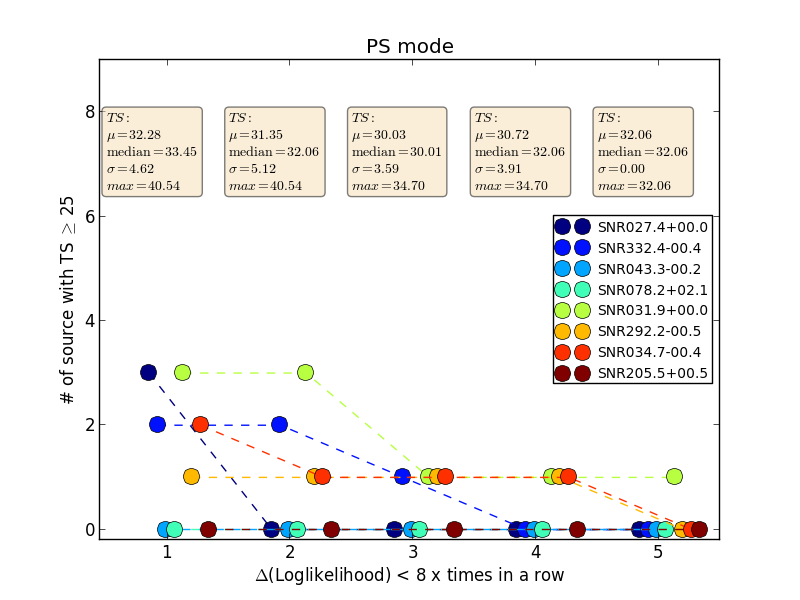
\includegraphics[width=1.0\columnwidth]{Figures/aboveThreshPSgt25.png}}
	\caption[Histogram of the number of signiciant soures remaining in each of the 8 test \roi{} for iterations in which $\Delta(\logL) < 8$]{Histogram of the number TS $\geq$ 25 sources remaining in each of the 8 test \roi{} for iterations in which $\Delta(\logL) < 8$ (\ie{} TS $<$ 16). Points are offset for each SNR for clarity. The text boxes detail statistics for the values of TS of significant sources for the 8 studied SNRs for each corresponding value on the x-axis.}
	\label{fig:NTSthresh}
\end{figure}

\begin{figure*}[ht]
	\begin{center}
		\hspace*{-1.5cm} \begin{tabular}{ll}
			\includegraphics[width=8cm]{Figures/{ES_1_Flux_SNR078.2p02.1_ES_noColor}.png} &
			\includegraphics[width=8cm]{Figures/{ES_1_Index_SNR078.2p02.1_ES_noColor}.png} \\
			\multicolumn{2}{c}{\includegraphics[width=8cm]{Figures/{ES_1_Sigma_SNR078.2p02.1_ES_noColor}.png}}\\
		\end{tabular}
	\end{center}
	\caption[SNR Gamma Cygni flux, index, and extension evolution for successive \srcs{} iterations]{
		\label{fig:gamCygEvo}{Flux (upper left), \pl{} spectral index (upper right), and extension (lower panel) evolution of the extended source coincident with \snr{} gamma Cygni (labeled ES 1 in the figures) as successive sources are added to the \roi{}.  Dotted line is first time $\Delta(\logL) < 8$, dashed line shows the final threshold for this test study.}
	}
\end{figure*}


To allow for proper convergence of the likelihood fit, we reduced the number of free parameters prior to each new source addition. If the previously added source was between $3$\degr{} and $5$\degr{} of the center of the RoI, just its normalization was freed, and if greater than $5$\degr{} all its source parameters were fixed.
To avoid having newly added sources overlap with pulsars, we deleted new sources from the RoI if they were within~$0.2$\degr{} of a \g-ray pulsar and refit the pulsar in the $1-100$\,GeV range following the 2PC conventions. 
2PC modeled pulsar spectra as a PL with an exponential cutoff (PLEC),
\begin{equation}
\newcommand{\pfrac}[2]{\left(\frac{#1}{#2}\right)} \frac{dN}{dE} = N_0 \pfrac{E}{E_0}^{-\Gamma} \exp\left(-\frac{E}{E_c}\right)^{b},
\label{eqn:PLEC}
\end{equation}
where \textit{$N_0$} is the normalization factor, \textit{$\Gamma$} is the photon spectral index, \textit{$E_c$} the cutoff energy, and $b$ determines to the sharpness of the cutoff. 2PC assessed the validity of fixing $b$ to $1$ in Equation~\ref{eqn:PLEC} (PLEC1) by repeating the analysis using a PL model, as well as the more general exponentially cut off PL form, allowing the parameter $b$ in Equation~\ref{eqn:PLEC} to vary. For the pulsar spectra in this analysis, we compared the maximum likelihood values for spectral models with and without a cutoff and with and without the value of $b$ being free, via $\mathrm{TS_{cut}} \equiv 2 ($\logL{}$_{\mathrm{PLEC1}}-$\logL{}$_{\mathrm{PL}})$ and $\mathrm{TS}_{b} \equiv 2 ($\logL{}$_{\mathrm{PLEC}}-$\logL{}$_{\mathrm{PLEC1}})$ to determine which to use. If $\mathrm{TS_{cut}} < 9$ is reported for the pulsar in 2PC then a PL model is used. If TS$_{\mathrm cut} \geq 9$, we then check to see if the cutoff energy fit in 2PC lies within the restricted energy range of $1-100$\,GeV used in this work. For pulsars with cutoffs $\geq 1$\,GeV, we then use the PLEC model if TS$_{\mathrm b} \geq 9$, and the PLEC model with cutoff freed otherwise. For those pulsars with cutoffs less than 1 GeV the spectral parameters are fixed to the 2PC values.

To complete the construction of our point source RoI model, we took the output of the previous steps and removed all sources with TS~$< 16$. This final model was then used as the starting model for analyzing candidate SNR emission. In Figure \ref{fig:w44initRoi}, we show a residual TS map of the region around \snr{} W44 as an example of the source configuration in an \roi{} prior to running \srcs{}. Figure \ref{fig:w44finRoi} is a residual \ts{} map of the same region after running \srcs{} to decompose the region into point sources.

\begin{figure}[ht!]
	\centering
	\makebox[\linewidth]{\includegraphics[width=1.0\columnwidth]{figures/{PS_00_tsmap_wo2FGL_SNR034.7-00.4_PS}.png}}
	\caption[1-100GeV  residual TS map for \snr{} W44 before running \srcs{} and with 2FGL sources removed from the inner 3$^\circ$ radius.]{1-100GeV  residual TS map for \snr{W44} before running \srcs{} and with 2FGL sources removed from the inner 3$^\circ$ radius (yellow circle). Bin size is 0.2°/pixel. Magenta circle shows a 5$^\circ$ radius. 2FGL and newly added sources are shown as green crosses.}
	\label{fig:w44initRoi}
\end{figure}

\begin{figure}[ht!]
	\centering
	\makebox[\linewidth]{\includegraphics[width=1.0\columnwidth]{figures/{TSgt16_tsmap_wo2FGL_SNR034.7-00.4_PS}.png}}
	\caption[1-100GeV  residual TS map for \snr{} W44 after \srcs{} has completed.]{1-100GeV  residual TS map for \snr{} W44 after \srcs{} has completed. 2FGL sources have been removed from the inner 3$^\circ$ radius (yellow circle), and the bin size is 0.2°/pixel. Magenta circle shows a 5$^\circ$ radius. 2FGL sources are shown as green crosses.}
	\label{fig:w44finRoi}
\end{figure}

We conservatively allow sources with TS down to $16$ $(\sim4\,\sigma)$ in order to account for the effects of at least the brightest sub-threshold sources on the parameter fits for the other sources in the model. Furthermore, while the SNR analysis method described in the chapter \ref{snrcat:DetectMethod} is allowed to remove sources, it cannot add them. Thus we start from a set of sources designed to allow the final model to capture all significant emission within the central region. To corroborate our method of systematically adding sources to a region, we compare our RoI source models with those found by the 2FGL approach in Chapter \ref{snrcat:addSrcs2FGL}. 



%%%%%%%%%%%%%%%%%%%%%%%%
%%%%%%%%%%%%%%%%%%%%%%%%

\section{Comparison of Source Models with 2FGL}
\label{snrcat:addSrcs2FGL}
This SNR catalog was constructed using $3$~years of P7 Source class data in the energy range $1-100$\,GeV, whereas 2FGL used $2$\,years of data over the larger energy range $0.1-100$\,GeV. The differences in observing time and energy range resulted in residual, unmodeled emission in some RoIs as well as changes to some 2FGL sources' spectral model, position localization, and detection significance. Here we compare the input source models constructed for this catalog, described in Chapter \ref{snrcat:AddSrcs}, with 2FGL to better understand the \srcs{} method's ability to describe the regions studied. Since we rederive the input source model only within a $3\degr$\,radius of the center of each RoI, we consider sources only inside that radius.

Given the data set differences, in each RoI we expect similar but not identical numbers of sources relative to those in 2FGL.
Figures~\ref{fig:2FGLvAddSrcs} and \ref{fig:2FGLvAddSrcsAssoc} show the numbers of significant (TS\,$\geq 25$) 2FGL sources and derived input model sources (excluding 2FGL identified AGN and pulsars kept in the input model) in individual RoIs as 2D histograms. In Figure~\ref{fig:2FGLvAddSrcs}, the number of sources in the derived input model is typically greater than the number of 2FGL sources that are significant at $1-100$\,GeV. 73 of the 279 RoIs studied contain at least one of the the 12 extended 2FGL sources. Since 2FGL extended sources were removed from the inner $3\degr$ of each RoI, and this region was repopulated with point sources, we can detect multiple point sources inside the extent of any removed extended 2FGL sources. This decomposition of extended sources, combined with the longer data set and different energy range compared to 2FGL, contribute to the high ratio of input model to 2FGL sources in some RoI, which demonstrates the need to rederive the source model. 

\begin{figure}[h!]
	\centering
	\makebox[\linewidth]{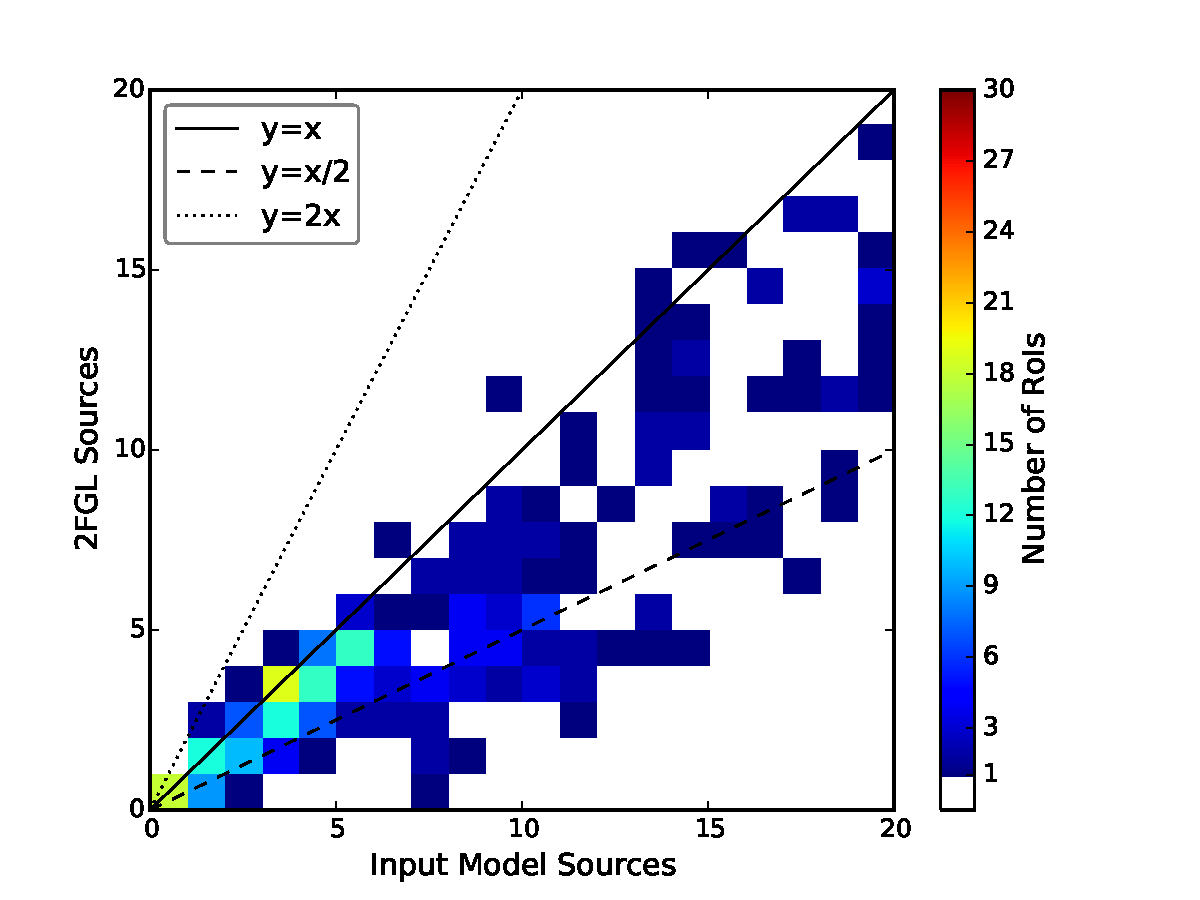
\includegraphics[width=1.0\columnwidth]{figures/addSrcs_2FGLnoAGNPSR_TSgt25_in3deg_2dhist_maj.pdf}}
	\caption[Comparison of the number of 2FGL sources with with the number of newly added input model sources.]{Comparison of the number of 2FGL sources with TS$_{1-100\,\mathrm{GeV}} \geq 25$ (excluding AGN and pulsars) with the number of newly added input model sources in the present analysis, for sources within $3$\degr{} of the center of each RoI. The color scale shows the number of RoIs with a particular combination of numbers of 2FGL sources and new sources. White corresponds to no RoI with that combination of source counts.}
	\label{fig:2FGLvAddSrcs} 
\end{figure}

To more accurately represent the 2FGL sources being reproduced in the central $3\degr$, in Figure~\ref{fig:2FGLvAddSrcsAssoc} we limited the input model sources to those within $0.2\degr$ (approximately the width of the core of the $10$\,GeV PSF) of a 2FGL source, effectively excluding input sources that are not co-spatial with a 2FGL source. Here we see that the majority of 2FGL sources have counterparts in the rederived set. As a region's complexity increases, seen as an increase in numbers of 2FGL sources, up to about half of the 2FGL sources may not have counterparts within $0.2$\degr. Given that in these same regions we have more new sources than 2FGL sources, as seen in Figure~\ref{fig:2FGLvAddSrcs}, we find as expected that the longer data set with improved statistics at higher energies, where the angular resolution of the LAT is the best, allows us to add new sources to account for newly significant excesses in these complex regions. Additionally, sources with low TS in 2FGL are particularly susceptible to having a newly added source which may start at a similar position but then localize further than $0.2\degr$ from the 2FGL source. 

Thus, we find that the method developed and used here produces a model which reproduces the 2FGL sources as expected, including differences that trend as anticipated given the longer data set and modified energy range, yielding better spatial resolution. The new method thus provides reasonable representations of the regions being modeled as input for the final analysis.

\begin{figure}[h!]
	\centering
	\makebox[\linewidth]{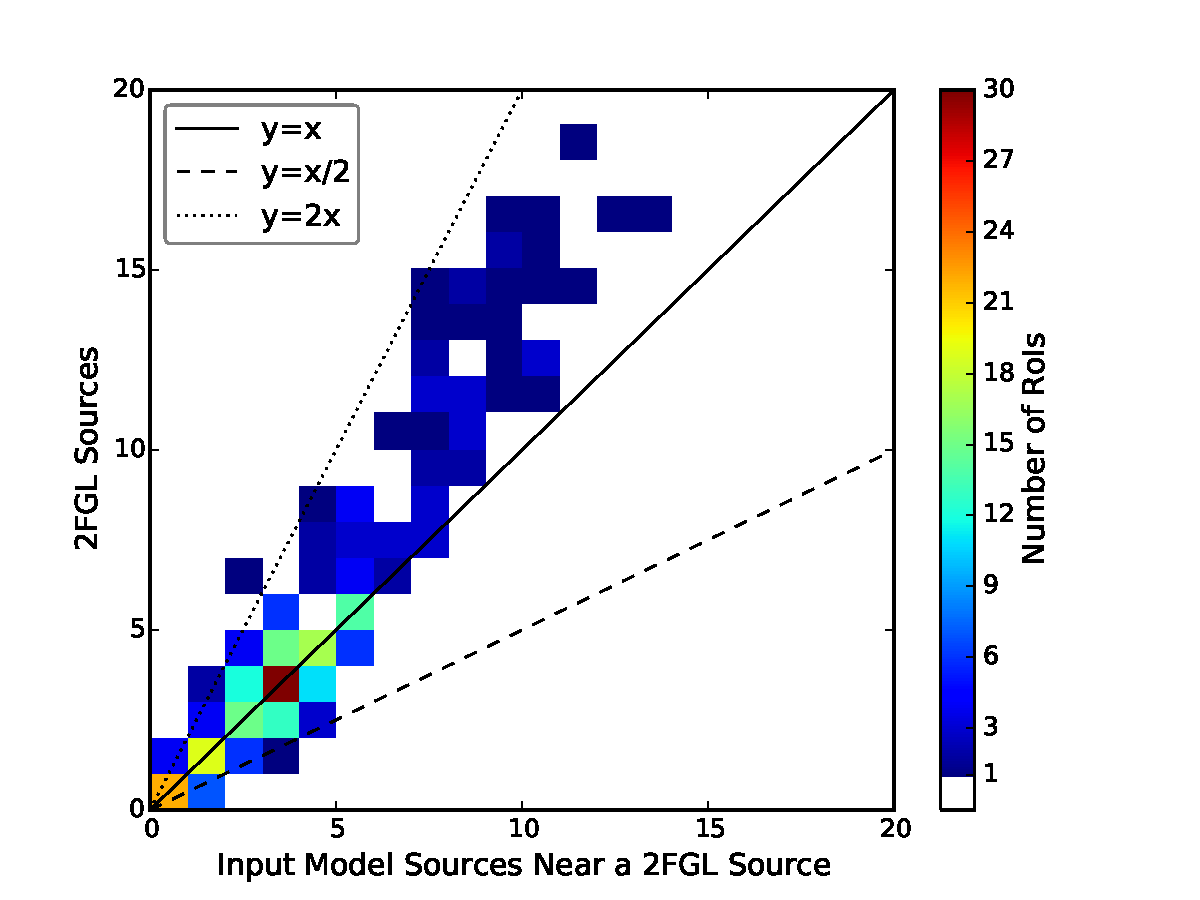
\includegraphics[width=1.0\columnwidth]{Figures/addSrcsWassoc_2FGLnoAGNPSR_TSgt25_in3deg_2dhist_maj.pdf}}
	\caption[Same as Figure~\ref{fig:2FGLvAddSrcs}, including only input model sources lying within $0.2$\degr{} of a 2FGL source.]{Same as Figure~\ref{fig:2FGLvAddSrcs}, including only input model sources lying within $0.2$\degr{} of a 2FGL source.}
	\label{fig:2FGLvAddSrcsAssoc} 
\end{figure}

%%%%%%%%%%%%%%%%%%%%
%  ANALYSIS SECTION
%%%%%%%%%%%%%%%%%%%%

\section{Detection Method}\label{snrcat:DetectMethod}
For each SNR, we characterize the morphology and spectrum of any \gam{} emission that may be coincident with the radio position reported in Green's catalog. This was achieved by testing multiple hypotheses for the spatial distribution of \gam{} emission: a point source and two different algorithms for an extended disk. The best fit was selected based on the global likelihoods of the fitted hypotheses and their numbers of degrees of freedom. The hypothesis with the best global likelihood was then evaluated using a classification algorithm described in \cite{snrCat} to determine whether the radio SNR could be associated with the detected \gam{} emission. 

Spatial coincidence is a necessary but not sufficient criterion to identify a \gam{} source with a known SNR. The detection of spatially extended \gam{} emission increases confidence in an identification, especially if GeV and radio sizes are similar, as has been observed on an individual basis for several extended SNRs \citep[e.g.][]{Lande12}. The LAT has sufficient spatial resolution to detect many Galactic SNRs as extended. Figure~\ref{fig:size_hist_p} shows the distribution of radio diameters from Green's catalog. Vertical dashed lines show the minimum detectable extension for sources with flux and index typical of those observed in this catalog, based on simulations using the P7V6 IRFs~\citep{Lande12}. The minimum detectable extension depends not only on the source's flux and spectrum, but also the flux of the background, which was estimated by scaling the average isotropic background level by factors of 10 and 100 to be comparable to the Galactic plane. As figure~\ref{fig:size_hist_p} illustrates, roughly one third of the known Galactic SNRs may be resolved by the LAT if they are sufficiently bright GeV sources.

\begin{figure}[h!]
	\centering
	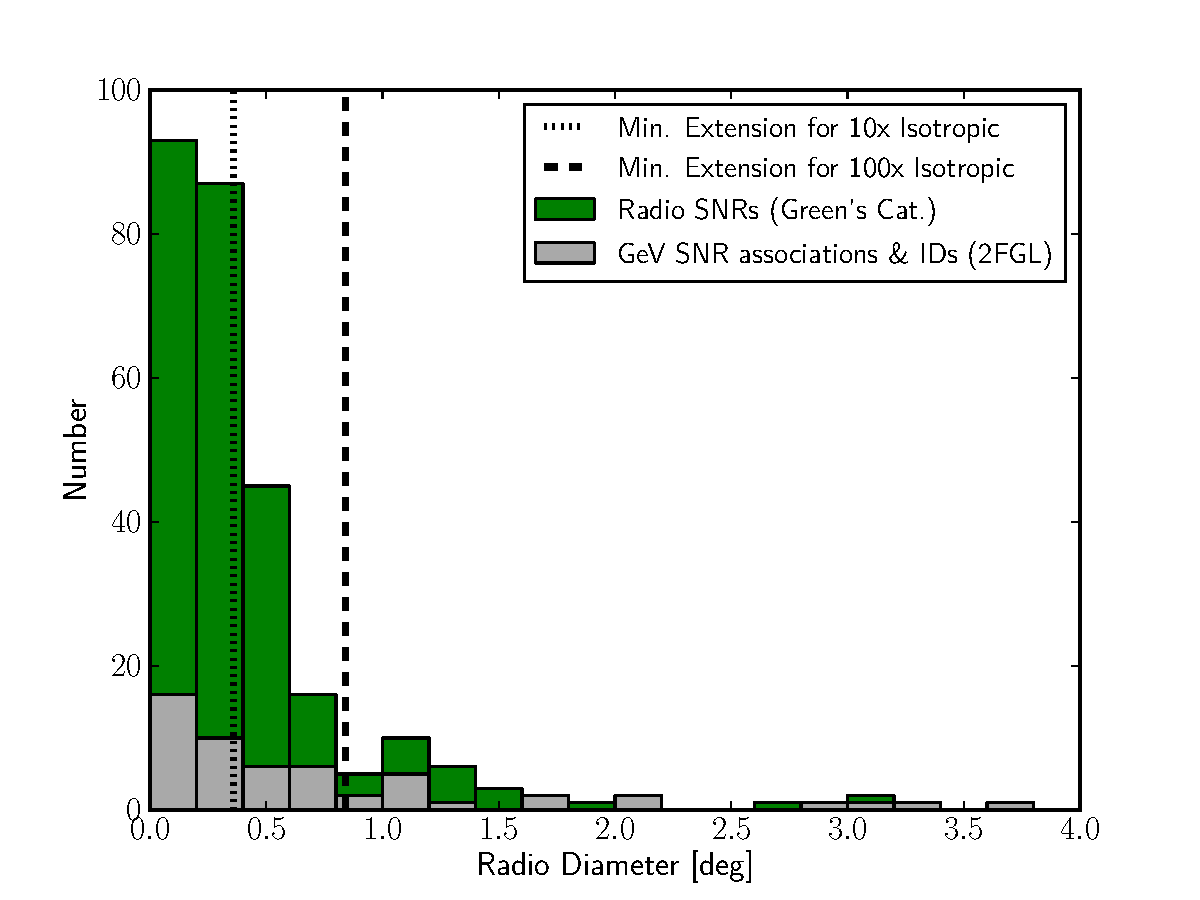
\includegraphics[width=1.0\columnwidth]{figures/size_hist_p.pdf} 
	\caption[Distribution of SNR radio diameters from Green's catalog]{Distribution of SNR radio diameters from Green's catalog. The vertical dashed lines indicate the minimum detectable extension for a source with a photon flux of $10^{-8}$\,ph\,cm$^{-2}$\,s$^{-1}$ in the $1-100$\,GeV energy range and a PL index of $-2.5$, from simulations of $2$\,years of data and the P7V6 IRFs \citep{Lande12}. In that work, simulations using $10$x and $100$x the isotropic background level (thin-dotted and thick-dashed lines) are used to estimate a reasonable background range for sources in the Galactic plane.\jamie{idk what plots are ok or not to include from papers I am an author on. I didnt make this plot, but I made the first version of it that inspired this one. Should I specifically include a comment for these plots that state they're from the snr cat vs ones not in the paper?}}
	\label{fig:size_hist_p}
\end{figure}

In order to determine the best representation for each SNR, we analyzed each SNR-centered RoI using multiple hypotheses for the spatial and spectral form. We used \ptlike{}~\citep{Kerr10} to compare PL and logP spectral forms, to compare point source versus extended source hypotheses, and to analyze the robustness of sources near the extended source.

For each hypothesis, we started with the input model described in Chapters \ref{snrcat:Data} and~\ref{snrcat:AddSrcs}. We removed sources falling within the SNR's radio disk unless they had been identified as an AGN or pulsar, as described in Chapter \ref{snrcat:AddSrcs}. We then proceeded to evaluate the following point and extended source hypotheses. For the point source hypothesis, a point source with a PL index initialized to $2.5$ was placed at the radio centroid of the SNR. The positions, spectral index, and spectral normalization of the point source were then fit. As for the initial input model described in Chapter \ref{snrcat:AddSrcs}, we tested the source for spectral curvature. To test the extended source hypothesis, we employed two separate procedures. Both employed a uniform disk model initially placed at the center of the RoI with a radius equal to that observed in the radio. In the first procedure, called the ``disk" hypothesis, we fit both the position and extension of the disk, as well as tested for spectral curvature. A second procedure, which results in a model we call the ``neardisk" hypothesis, additionally examines the significance of sources nearby the disk, removing those which are not considered independently significant and refitting the disk position and radius. This procedure is described in Chapter \ref{snrcat:LocExtSpec}.

Having evaluated these hypotheses, we compared the global likelihood values of the final extended hypothesis and of the point source hypothesis to determine which model had the largest maximum likelihood. If the source is significant in the best hypothesis, the model parameters are reported as Tables 1 and 2 in \cite{snrCat} \jamie{should I include abridged tables?}. If no hypothesis had a significant \gam{} source coincident with the radio SNR, we calculated the upper limit on the flux from a region consistent with the radio SNR, described in Chapter \ref{snrcat:FluxULs}, and report  the results in Table 3 in \cite{snrCat}. \jamie{should I include the tables here? only if they're short, or abridged. I should def include the dist table because I did that work}

\subsection{Localization, Extension, and Spectral Curvature}\label{snrcat:LocExtSpec}
To test our hypotheses, we combined the initial model of point sources (Chapter \ref{snrcat:AddSrcs}) and the Galactic and isotropic diffuse contributions (Chapter \ref{snrcat:Data} and \ref{snrcat:AddSrcs}) with a test source at the center of each RoI. All sources that fell within the radio SNR radius other than previously identified AGN or pulsars were removed, as was done for the input source model (Chapter \ref{snrcat:AddSrcs}). We note that multiple point sources removed within a single radio SNR radius may represent substructure within the source itself. This process conservatively assigns the majority of the flux to a single source, rather than decomposing it. We optimized the position of the test source with \ptlike{}, iteratively allowing other model parameters to vary. For all hypotheses, the normalizations of all sources within $5$\degr{} of the radio SNR center were fit while all other spectral parameters were fixed. The parameters for sources outside $5$\degr{} were also fixed.

For the point source hypothesis, a point source was placed at the radio centroid of the SNR. For the disk hypothesis, a uniform disk with radius equal to the radio radius was placed at the center. In both hypotheses, the normalization, index, and position of the candidate source were fit. For the disk hypothesis, the extension was also fit. Previous analyses of a range of possible Galactic SNR sources with similar data sets \citep[e.g.][]{Lande12} typically showed no differences in global likelihood significant enough to justify choosing a Gaussian over a uniform disk template or vice versa. In addition, there was typically little difference in spectral parameters for the two spatial forms. For simplicity and clarity, we thus test only the uniform disk hypothesis. We allowed the localization to wander up to  $5$\degr{} in the fits as a reasonable upper limit on what might later be associated with the SNR. This is roughly twice the radius of largest radio SNR.

We included an additional disk hypothesis in which we recalculated the significance of each nearby point source. Because neighboring sources can influence the best fit disk parameters, we iteratively evaluated the significance of the neighboring source by calculating TS$_{\rm nearby}$, defined as twice the difference between the model's log-likelihood (\logL{}) with the nearby point source and the model without the source, as determined by \ptlike. Starting from the fitted disk model, for each neighboring point source we refit the position, extension, normalization, and spectrum of the uniform disk after removing the source. A nearby source was considered to be significant and thus kept if TS$_{\rm nearby} \geq 9$. Each point source was evaluated individually, starting with the closest point source and extending radially outward to all sources within $1$\degr{} of the furthest edge of the SNR's radio disk. The final result of this iterative process is called the ``neardisk" hypothesis which, for cases where neighboring source(s) were removed, can have different best fit disk parameters. As a final step we refit the region with \gtlike, using the neardisk model.

We chose the best extended source hypothesis by comparing the final disk and neardisk \gtlike{} \logL{} values. Since the neardisk hypothesis can have fewer degrees of freedom, we chose the final disk hypothesis only if $2\times$(\logL{}$_{\rm disk}$-\logL{}$_{\rm neardisk}$) $\geq 9$. Otherwise, we used the neardisk model as the final extended source hypothesis, hereafter referred to as the ``disk hypothesis''.

In some cases a point source could not be localized starting at the SNR center. If the \ptlike{} localization failed to converge when starting at the SNR center, we placed the candidate at the position of the most significant source removed from within the radio SNR radius and followed the procedure outlined above. For $69$~RoIs there was either no source removed within the radio SNR or localization failed. For $31$~RoIs, the candidate found had a TS~$<1$ and was removed from the model so as not to cause instabilities in the minimization. If the disk hypotheses converged and the final candidate was significant (TS~$\geq 25$) in both the localization and spectral fits, the best extended hypothesis was selected. 

Prior to the final fit of the region, sources were tested for spectral curvature using $\mathrm{TS_{band fits} - TS_{PL}}\geq~25$. If this criterion was satisfied then we replaced the PL spectral model with a logP model and refit the RoI. The final spectral model was selected, as for the input model, by comparing the \logL{} values, in this case $\mathrm{TS_{curve}} \geq 16$, as defined in Chapter \ref{snrcat:AddSrcs}. Seven sources were found to be significantly better fit by a logP spectrum. To obtain final spectral parameters, we performed a final fit using the standard likelihood analysis tool \gtlike. The normalization and index parameters were constrained to lie within a physically reasonable range. 

%%%%%%%%%%%%%%%%%%%%%%%%%%%%%%%%%%%

We determined the final RoI model by selecting the most likely hypothesis based on a comparison of the \gtlike{} global \logL{} of the point source hypothesis with the most likely extended source hypothesis. An extended hypothesis was considered significantly more likely if $\mathrm{TS_{ext}}$ was $\geq 16$, where $\mathrm{TS_{ext}}$ is defined as twice the difference between the \logL{} of the final model from the disk hypothesis and that of the point source hypothesis, $\mathrm{TS_{ext}} =  2 ($\logL{}$_{\mathrm{disk}}-$\logL{}$_{\mathrm{point}})$, as in~\citet{Lande12}. Otherwise, if the point source itself had TS\,$>25$, we chose the point source hypothesis. In cases in which the optimization for the position of the point source did not converge but an extended disk was detected, we calculated the global \logL{} of the region without any source and with a point source at the center of the extended source. We then use the latter value to calculate $\mathrm{TS_{ext}}$ reported in Table 1 in \cite{snrCat}. For these candidates, if the source was significantly extended in both cases, we select the extended hypothesis. If none of the criteria were met, the candidate was considered undetected and we calculated an upper limit on the flux. Both the upper limits and flux calculation are described in the following subsection.

\subsection{Fluxes and Upper Limits}\label{snrcat:FluxULs}
Fluxes in the $1-100$\,GeV band are determined using the standard analysis tool \gtlike{} by a final fit of the model chosen to have the overall maximum likelihood characterization of the morphology and spectrum of the candidate source from the analysis detailed in Chapter \ref{snrcat:DetectMethod} and \ref{snrcat:LocExtSpec}. For those RoIs where no significant source was detected, we computed Bayesian upper limits on the flux using the method in described in \citet{Helene83} excluding any overlapping sources in the model that have not been identified as AGN or pulsars, as described in Chapter \ref{snrcat:AddSrcs}. As a spatial model we used a uniform disk equal in position and radius to that reported in Green's catalog. We assumed the spectral model to be a PL and report upper limits for indices of $2.0$ and $2.5$ at $95\%$ and $99\%$ confidence levels. The choice of indices was motivated by the distribution of PL indices for classified sources. The results are reported in \cite{snrCat}.

%%%%%%%%%%%%%%%%%%%%%%%%
%%%%%%%%%%%%%%%%%%%%%%%%

\section{Catalog Results}\label{snrcat:TheCatalog}
We detected \ndetected~candidates with a final source TS\,$\geq 25$ in the \nGalSNRs~SNR RoIs (see Chapter \ref{snrcat:DetectMethod}). Of the \ndetected~detected candidates, \nassocprobclassified{} passed the association probability threshold (see \cite{snrCat}). Of these, \nclassifiedsnrs~SNRs ($\sim11\%$ of the total) show significant emission for all alternative IEMs and are classified as likely GeV SNRs. An additional \nnotsnrs{} were identified as sources which are not SNRs.Two other candidates were demoted to marginal due to their dependence on the IEM, as described in the next paragraph. Of the sources likely to be GeV SNRs, \nextended~show evidence for extension (TS${\rm_{ext} > 16}$). Only sources associated with SNRs G34.7$-$0.4 and G189.1+3.0 show evidence of significant spectral curvature in the $1-100$\,GeV range and are fit with logP spectra. Of the classified candidates, \nnewextended~extended and \nnewpointlike~point SNRs are new and published here for the first time. Descriptions of the new extended (G24.7+0.6, G205.5+0.5, G296.5+10.0, and G326.3$-$1.8) \snrs{} is given in \cite{snrCat}.
%We describe the \nnewextended~new extended SNRs, G24.7+0.6, G205.5+0.5, G296.5+10.0, and G326.3$-$1.8, in Section~\ref{snrcat:NewSNRs}. 

For those \nULs~SNRs that are either not detected by this analysis or which fail to meet the most stringent threshold for classification as a detected SNR, upper limits assuming the radio disk morphology of Green's catalog with PL indices of $2.0$ and $2.5$ are reported in Table 3 in \cite{snrCat}. For those candidates which fail to meet the most stringent threshold, we replaced the source with the radio disk. We do not calculate upper limits for the \nnotsnrs~sources which are identified as not SNRs. A FITS version of the catalog is available through the \Fermi{} Science Support Center, as described in \cite{snrCat}\footnote{\url{ http://fermi.gsfc.nasa.gov/ssc/data/access/lat/1st_SNR_catalog/}}. \jamie{not including the detailed description of the new SNRs}

\jamie{all the multiwavelength CR stuff and  I wasn't so involved in, but it's kind of the crux of the paper. I don't know how much of if it, if any to include here.}

%%%JAM COMMENTED OUT THESE TABLES
%\input{t1.tex} %{tables/results_v4_0516_det_spatial.tex}  % reference as \ref{Tab:ResultsSpat}
%\input{t2.tex} %{tables/fluxTable2_v7/results_v4_0516_det_spectral_v7.tex} % reference as \ref{Tab:ResultsSpec}
%\input{t3.tex} %{tables/results_v4_0516_UL.tex}   % reference as \ref{Tab:ResultsULs}

%%%%JAM commented this out for now
%\begin{figure}[h!]
%   \centering
%   \includegraphics[width=0.8\columnwidth]{f9.pdf} %{figures/gev_flux_vs_index.pdf}
%   \caption{
%       The distribution of fitted photon index and flux in the energy range $1-100$\,GeV. The index shown for sources for which the logP form is more significant is determined from re-fitting the sources with a PL spectral form rather than their parabolic index $\alpha$, for consistency. Open circles indicate extended SNRs while filled circles indicate point-like sources. All SNRs that passed classification are shown as black unless also classified as young non-thermal X-ray SNRs (blue) or as interacting with MCs (red). Candidates which did not pass classification but still had both fractional overlaps $>0.1$ are grey. If they are also young or interacting, they are outlined in blue or red, respectively\protect\footnotemark. These classes are further defined in Section~\ref{Sec:GeVSNRDiscussion}. Statistical error bars have caps; error bars without caps represent the systematic error, described in Section~\ref{Sec:SysErr}. 
%       \label{fig:GeVFluxGeVIndex}}
%\end{figure}
%\footnotetext{No extended marginally classified candidates were also identified as young or interacting.} 


%%%%%%%%%%%%%%%%%%%%%%%%
%%%%%%%%%%%%%%%%%%%%%%%%

\section{GeV Supernova Remnants in a Multiwavelength Context: Discussion Summary}\label{snrcat:resSum}
\emph{Here, we summarize some of the findings detailed in the \snrcat{} that are most pertinent to the work performed for this thesis.} \jamie{do I need a statement like  this?}

As discussed in Chapter \ref{gamAstr:CR}, the same population of radio, synchrotron-emitting \cray{} electrons active in the shell of an \snr{} are expected to also produced \gam{}s through the \ic{} process and non-thermal \brems{} radiation. If indeed the\gev{} and radio emission are produced in a single zone, it is reasonable to assume that the radio and \gam{} morphologies will correlate. We find that the best GeV diameter is within errors of the radio diameter for most of the candidates classified as being associated with an SNR, as shown in Figure \ref{fig:GeVradioSize}. The same, co-spatial, electron population producing the\gev{} and radio emission is also suggestive of a potential correlation between the radio and \gam{} flux. Figure \ref{fig:GeVradioFlux} shows the 1 GHz synchrotron flux versus the 1\gev{} \gam{} flux for all \snrs{}. Despite suggestions of correlation, Kendall’s $\tau$ rank correlation tests suggested no significant correlation exists between the radio and GeV flux or luminosities (not shown here). Various factors, such as the lack of detailed nonthermal emission modeling, distance measurement errors, and use of oversimplified \gam{} spectral models can skew these results, obscuring any inherent correlation.

\begin{figure}[h!]
	\centering
	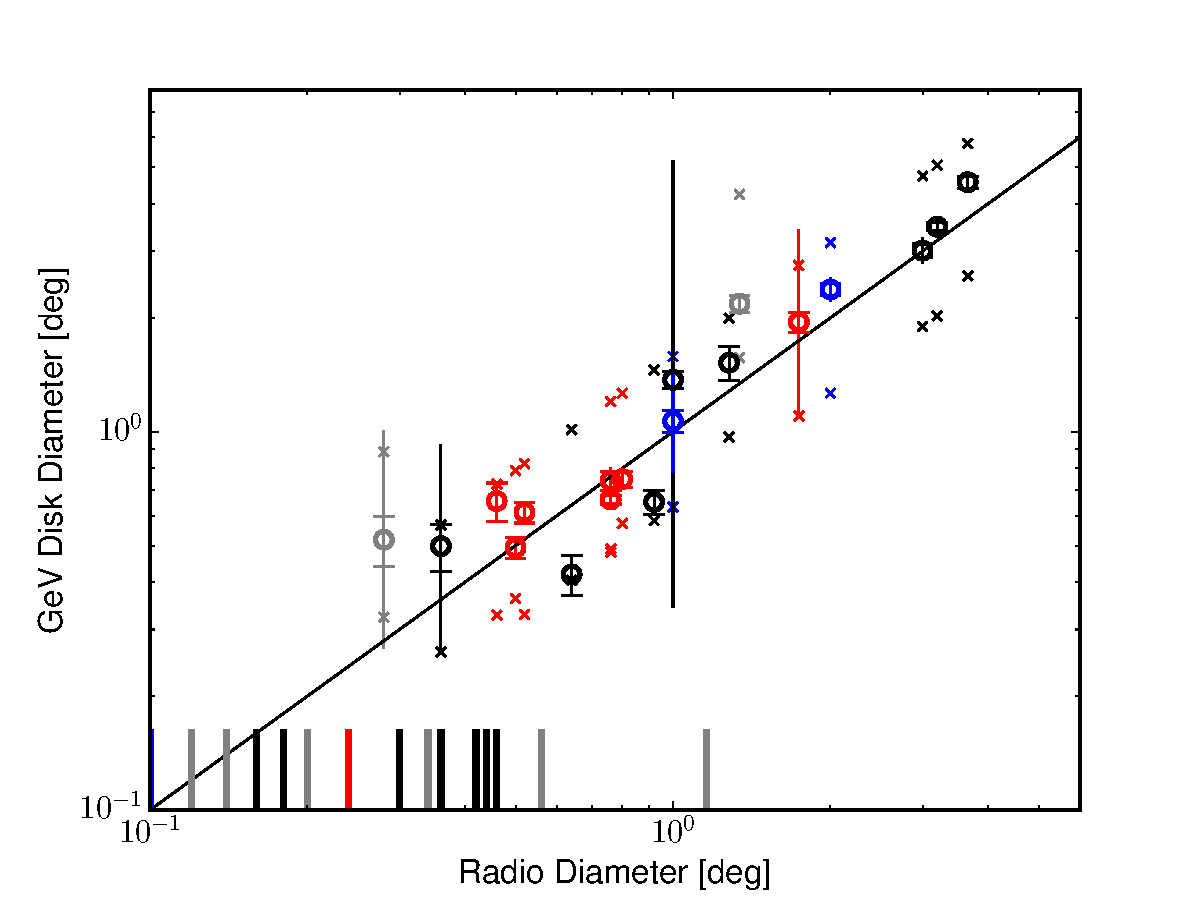
\includegraphics[width=1.\columnwidth]{figures/size_radio_vs_gev_xLims.pdf}
	\caption[Radio diameter of Green's catalog SNRs plotted against the fitted GeV diameterß]{Radio diameters of Green's catalog SNRs plotted against the fitted GeV diameters for those candidates with significant extension. The solid line represents equal radio and GeV diameters. All cases of detected extension have diameters greater than $0.2$\degr. The ticks denote the radio extension of GeV point-like candidates, colored in order of their characteristics (young or interacting) and by their classifications (well defined or marginal). The small `x's bracketing the points show the minimum and maximum GeV extensions allowed such that the source remains classified or marginally classified  given the radio position and extension and best fit GeV position. Open circles indicate extended SNRs. All SNRs that passed classification are shown as black unless also classified as young, nonthermal X-ray SNRs (blue) or as interacting with MCs (red). Candidates that did not pass classification but that still had both fractional overlaps $>$ 0.1 are gray.  Statistical error bars have caps; error bars without caps represent the systematic error. \jamie{took out the filled circles and outlined part,  If they are also young or interacting, they are outlined in blue or red, respectively (No extended marginally classified candidates were also identified as young or interacting.)}}
	\label{fig:GeVradioSize}
\end{figure}

\begin{figure}[h!]
	\centering
	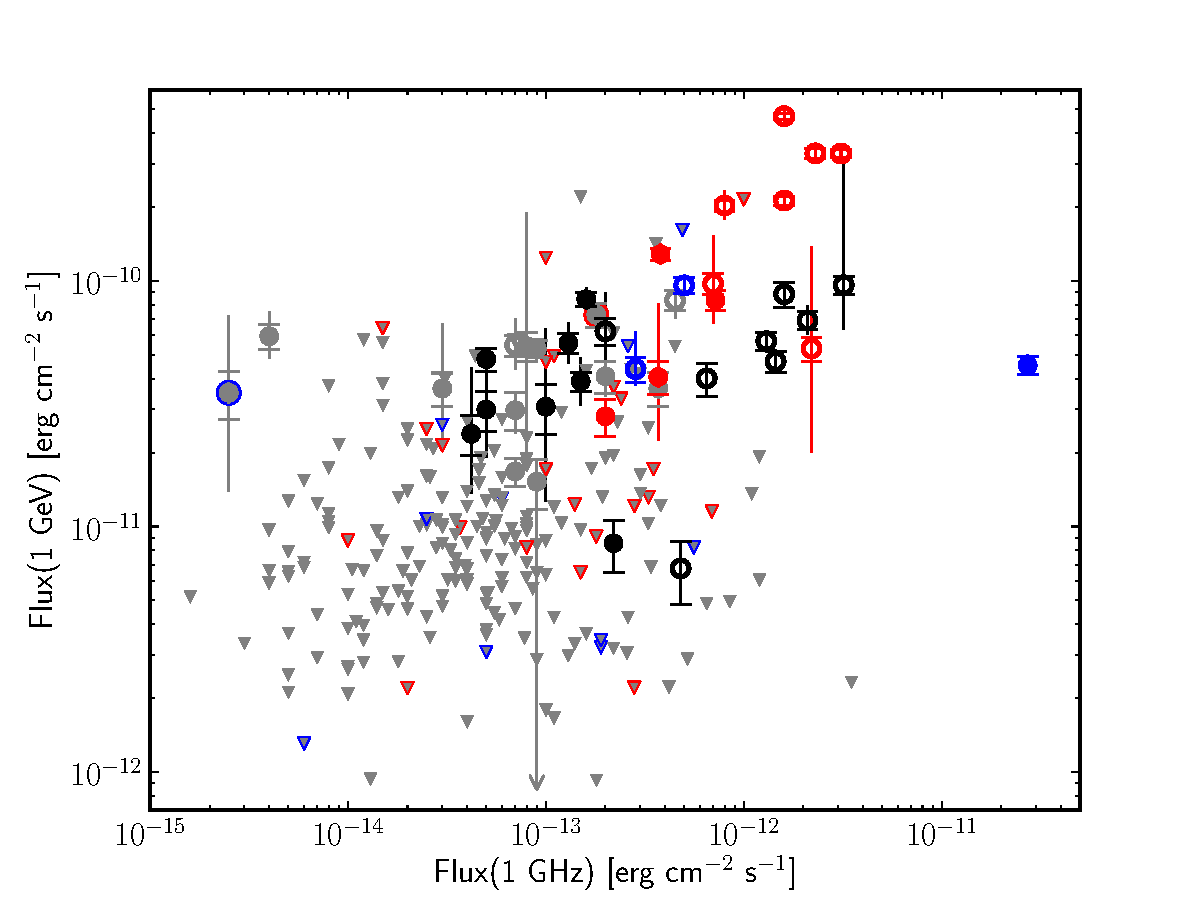
\includegraphics[width=1.\columnwidth]{figures/radio_vs_gamma_nuFnu_flux_ULs.pdf}
	\caption[Comparison of \gam{} and radio spectral flux densities for all SNRs and candidates.]{Comparison of \gam{} and radio spectral flux densities for all SNRs and candidates. For all SNRs that were not detected or which failed classification, grey triangles indicate upper limits at $99\%$ confidence, computed assuming the radio location and extension. Symbols, colors, and error bars are as in Figure \ref{fig:GeVradioSize}. In addition, filled circles indicate point-like sources, and if grey markers are also young or interacting, they are outlined in blue or red, respectively (No extended marginally classified candidates were also identified as young or interacting).
	}
	\label{fig:GeVradioFlux}
\end{figure}

We test for one further relationship between the radio and GeV emission and the underlying particle populations through the measured radio and GeV spectral indices. The energy of synchrotron-emitting leptons traced by $1$\,GHz observations depends on the magnetic field. If radio and GeV emission trace the same underlying particle population, then, at energies below the maximum energy reached by the accelerated particles, the photon indices of radio and \gam{} emission should be correlated. For $\pi^0$ decay and e$^\pm$ bremsstrahlung, the GeV and radio photon indices ($\Gamma$ and $\alpha$ respectively) are related as $\Gamma = 2\alpha + 1$. For IC scattering leptons, the GeV and radio photon indices follow $\Gamma = \alpha + 1$, or in the case in which high-energy leptons have been cooled via synchrotron or IC radiation, $\Gamma = \alpha + 3/2$ \citep{Reynolds08}. Figure \ref{fig:GeVradioIndex} compares the deduced radio spectral index $\alpha$ with the $1-100$\,GeV photon index $\Gamma$. 

\begin{figure}[h!]
	\centering
	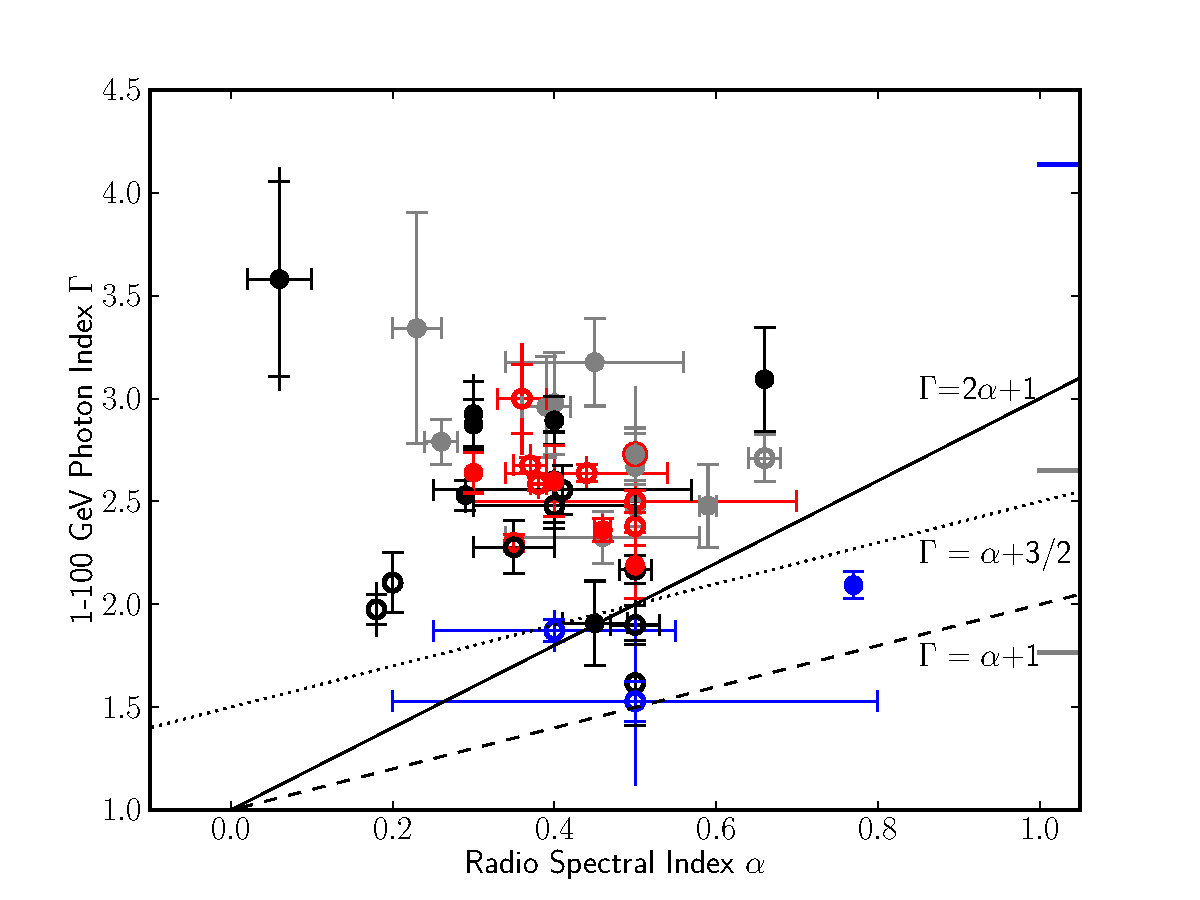
\includegraphics[width=1.0\columnwidth]{figures/radio_vs_gamma_index.pdf}
	\caption[Comparison of radio spectral index, $\alpha$, and GeV photon index, $\Gamma$.]{Comparison of radio spectral index, $\alpha$, and GeV photon index, $\Gamma$. The expected correlations are plotted for $\pi^0$ decay or e$^{\pm}$ bremsstrahlung (solid) and IC emission from an electron population that is freshly accelerated (dashed) or cooled by radiative processes (dotted). Emission via a combination of processes would fall between the lines (e.g. between the solid and dashed for a combination of $\pi^0$ decay and IC emission).  Symbols, colors, and error bars are as in Figure \ref{fig:GeVradioSize}; ticks along the right hand side show the $1-100$\,GeV photon indices of those SNRs without reported radio spectral indices.
	}
	\label{fig:GeVradioIndex}
\end{figure}

Nearly all candidates have \gam{} photon indices that are softer than predicted given their radio spectra, regardless of the GeV emission mechanism. The three young SNRs in blue are most consistent with a single underlying particle population, and it has been suggested they emit via IC (dashed line) at GeV energies. SNRs emitting via a combination of mechanisms under these simple assumptions would have indices falling between the two index relations, that is, they would lie in the region spanned by the $\pi^0$/bremsstrahlung (solid) and IC (dashed) lines. 

The lack of an observed correlation between the indices as expected under these simple assumptions suggests that more detailed physical models are required for the majority of SNR candidates. The observed soft GeV spectra relative to the radio has several potential explanations. 
The underlying leptonic and hadronic populations may have different PL indices. The emitting particle populations may not follow a PL but may instead have breaks or even differing spectral shapes. Finally, there may be different zones with different properties dominating the emission at different wavelengths.

In the \snrcat{}, we also compared the GeV and TeV properties of SNRs to test the second common assumption in SNR models: that momentum distributions of the emitting particle populations do not follow simple PLs but have curvature or breaks. Such changes in spectral slope could also cause breaks in the \gam{} spectra. As TeV emission may originate via the same processes as the \FermiLat-observed GeV emission \citep[e.g.][]{Funk08_GeVTeVGalactic, Tibolla09_HESSUnIds, Tam10_VHEforFermi}, we might expect to see such a change reflected in a spectrum combining \FermiLat{} data with observations from \iacts{} such as \hess{}, \veritas{}, and \magic{}. The converse is also true, where detection predictions in the GeV based on simple PL extrapolation from the TeV have been borne out in GeV studies, e.g. identifications of H.E.S.S. sources from \cite{Tibolla09_HESSUnIds} in 2FGL \citep{2FGL} and \cite{Ackermann12_1FGLUnassoc}. 

In Figure~\ref{fig:GeVTeVIndex} we plot the PL index in the GeV versus TeV range for all SNRs observed with both \FermiLat{} and an IACT detections. Six of the ten SNR candidates have TeV indices that are softer than their GeV indices, while three have GeV and TeV indices that are consistent with each other, within statistical and systematic errors. The remaining interacting candidate has a somewhat softer index at GeV energies than at TeV. Such a hardening of the index from GeV to TeV suggests that another particle population may dominate at higher energies or that the emission mechanism may change between the GeV and TeV regimes. Such curvature in the spectrum may also explain the lack of a simple correlation between GeV and radio PL indices, as described above in this section. We also note that Figure~\ref{fig:GeVTeVIndex} shows a distinct separation between young and interacting SNRs, which are often older. This suggests an evolution in index with age, from harder when younger to softer when older. 

\begin{figure}[h]
	\centering
	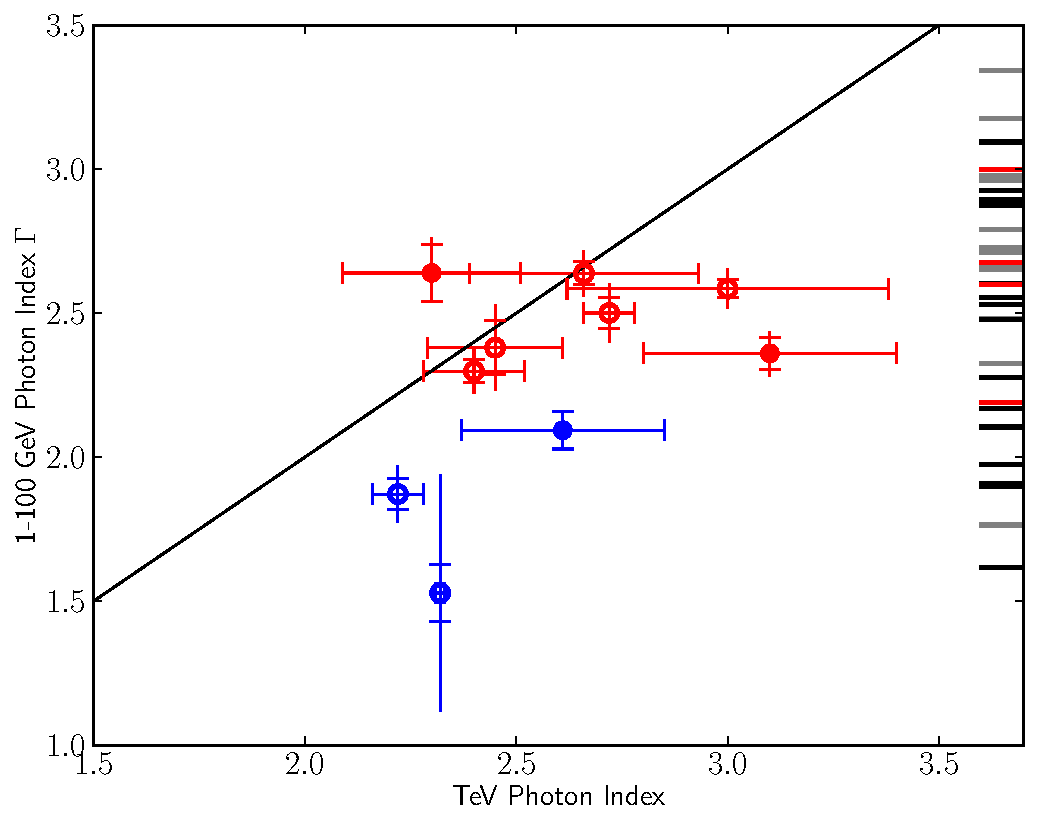
\includegraphics[width=0.8\columnwidth]{Figures/gev_vs_tev_index.pdf}
	\caption[GeV index compared to published index measurements from \iacts{}.]{GeV index compared to published index measurements from \iacts{}. The line corresponds to equal index values. The predominance of SNRs below the line suggests spectral curvature, potentially reflecting a change in spectral slope of the underlying particle population(s') index or indices. The ticks represent the GeV candidates with indices in the range of those with a TeV counterpart but with no TeV measurements themselves, demonstrating the limitations of the data set. Symbols, colors, and error bars are as in Figure~\ref{fig:GeVradioSize}. 
	}
	\label{fig:GeVTeVIndex}
\end{figure}

In Figure~\ref{fig:AgeGeVIndex}, we take SNR ages from the literature and plot the $1-100$\,GeV photon index versus age. For our uniform sample of all GeV SNR candidates, young SNRs tend to have harder GeV photon indices than interacting SNRs, which are likely middle aged, though the scatter in age for the two classes is one to two orders of magnitude. The general trend of younger SNRs having harder indices may be due to the decrease of the maximum acceleration energy as SNRs age and their shock speeds slow down. This would also result in fewer particles being swept up by the shock front, given a constant density, suggesting a corresponding decrease in luminosity with age.

\begin{figure}[h]
	\centering
	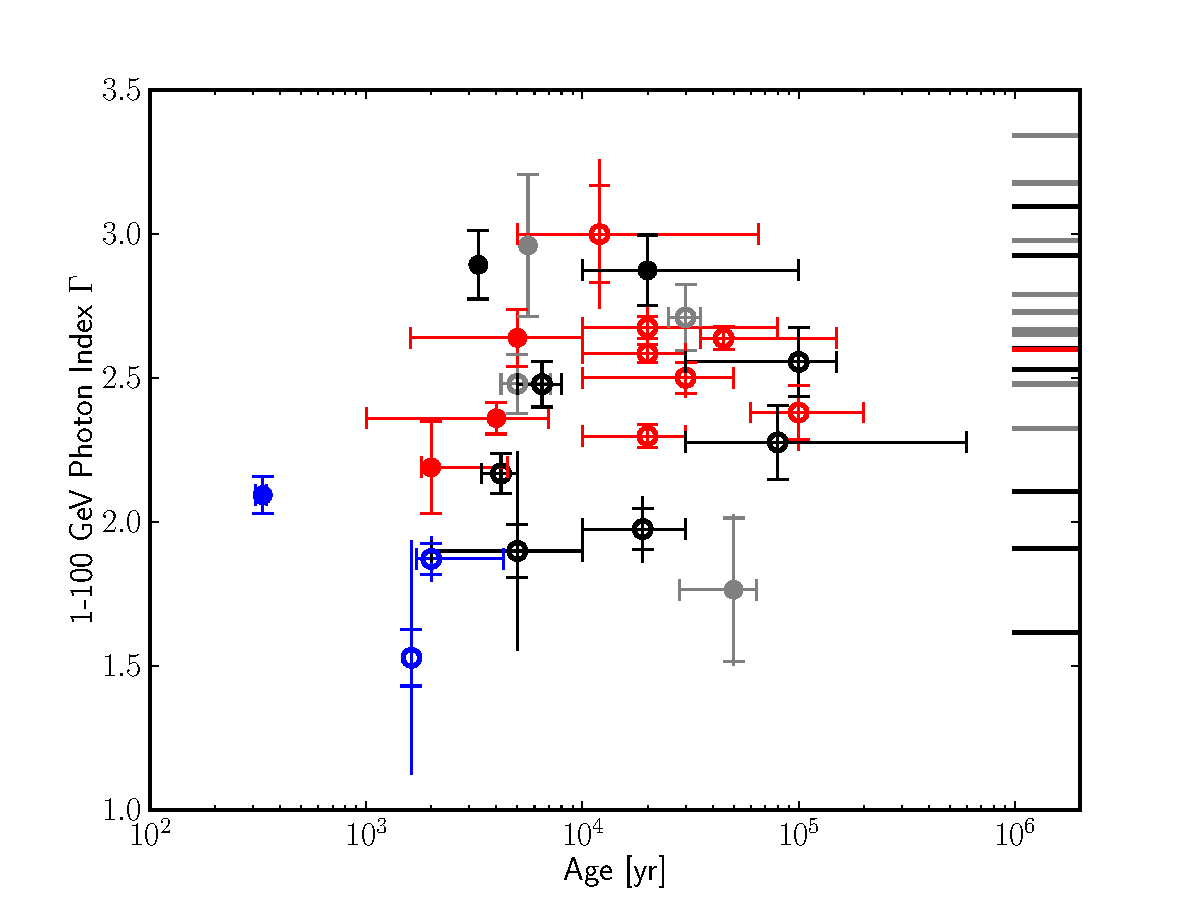
\includegraphics[width=1.0\columnwidth]{Figures/age_vs_index.pdf}
	\caption[Age versus GeV spectral index]{Age versus GeV spectral index. For those with ages in the literature, the young (blue) SNR candidates are separated in this phase space from the identified interacting candidates (red). The ticks on the right show indices for GeV candidates without well-established ages. Symbols, colors, and error bars are as in Figure \ref{fig:GeVradioSize}. 
		\label{fig:AgeGeVIndex}}
\end{figure}

It is important to account for the distances of the SNRs when comparing physical quantities such as luminosity. Table~\ref{Tab:SNRinfo}  records distance from the literature, including the most recent and/or most certain distance estimates adopted in this work. Of the \nGalSNRs~SNRs studied, only \ndist{} have published distance estimates. Most often these distances are determined from observed line-of-sight velocities using an assumed Galactic rotation curve. Furthermore, kinematic distance estimates have largely been done on an individual basis, and are not uniformly determined for all SNRs. We do not consider distances derived using the ``$\Sigma$-D relation" because SNRs show a wide range of physical diameters (D) for a given surface brightness ($\Sigma$), limiting the utility of such a relationship for determining the distances to individual SNRs \citep{Green12-distances}.

\pagestyle{empty}
\begin{deluxetable}{lcll}
	\setlength{\tabcolsep}{0.02in} 
    \tablewidth{0pt}
	\tabletypesize{\scriptsize}
	\tcap{Distances to SNRs \label{Tab:SNRinfo}}
	\tablehead{
		\colhead{Name} & 
		\colhead{d [kpc]} & 
		\colhead{Method} &
		\colhead{Reference(s)}
	}
\startdata
G000.0$+$00.0 & 8.5                           & IAU value & \cite{1986MNRAS.221.1023K} \\
G000.3$+$00.0 & 8.5$^{+3.0}_{-3.0}$          & H\,{\sc i} & \cite{2010ApJS..191..275L} \\
G000.9$+$00.1 & 8.5$^{+7.5}_{-1.5}$          & PSR & \cite{2009ApJ...700L..34C} \\
G001.0$-$00.1 & 8.5                           & Maser & \cite{1999ApJ...527..172Y} \\
G001.4$-$00.1 & 8.5$^{+5.6}_{-0.0}$          & Maser & \cite{1999ApJ...527..172Y} \\
G004.5$+$06.8 & 7.0$^{+2.0}_{-0.6}$          & H\,{\sc i} & \cite{1999AJ....118..926R}, \cite{2005AdSpR..35.1027S}, \cite{2008AA...488..219A} \\
G005.4$-$01.2 & 4.75$^{+0.45}_{-0.45}$       & Maser & \cite{2009ApJ...694L..16H} \\
G005.7$-$00.0 & 8.4$^{+5.3}_{-5.3}$          & Maser & \cite{2009ApJ...694L..16H} \\
G006.4$-$00.1 & 1.9$^{+0.4}_{-0.4}$          & Maser, CO & \cite{2002AJ....124.2145V} \\
G008.7$-$00.1 & 4.5                           & Maser & \cite{1990Natur.343..146K} \\
G009.7$-$00.0 & 4.7                           & Maser & \cite{2009ApJ...694L..16H} \\
G011.2$-$00.3 & 5$^{+21}_{-0.5}$             & H\,{\sc i} & \cite{1972ApJS...24...49R}, \cite{1985ApJ...296..461B}, \cite{1988MNRAS.231..735G} \\
G012.8$-$00.0 & 4.7$^{+1.3}_{-1.1}$          & PSR & \cite{2012ApJ...753L..14H} \\
G013.3$-$01.3 & 3.3$^{+1.8}_{-1.7}$          & CO & \cite{1995ApJ...449..681S}, \cite{1998AJ....116.1323K} \\
G015.1$-$01.6 & 5.7$^{+1.3}_{-3.5}$          & NH & \cite{2008AA...481..705B} \\
G015.4$+$00.1 & 4.8$^{+1.0}_{-1.0}$          & CO & \cite{2013AA...557L..15C} \\
G016.7$+$00.1 & 10.0$^{+3.7}_{-7.4}$         & Maser, CO & \cite{2008ApJ...683..189H}, \cite{2000ApJ...545..874R} \\
G016.8$-$01.1 & 5.1$^{+4.6}_{-1.8}$          & H\,{\sc i} & \cite{2011AA...536A..83S} \\
G018.1$-$00.1 & 5.58$^{+0.24}_{-0.27}$       & H\,{\sc i} & \cite{2014MNRAS.438.1813L} \\
G018.6$-$00.2 & 4.6$^{+0.6}_{-0.6}$          & H\,{\sc i} & \cite{2009AJ....138.1615J} \\
G018.8$+$00.3 & 12.0$^{+3.0}_{-5.1}$         & H\,{\sc i} & \cite{2007AA...474..541T} \\
G021.5$-$00.9 & 4.7$^{+0.4}_{-0.4}$          & PSR & \cite{2006ApJ...637..456C}, \cite{2008MNRAS.391L..54T} \\
G021.8$-$00.6 & 5.35$^{+0.15}_{-0.15}$       & CO, PSR & \cite{2008MNRAS.391L..54T}, \cite{2009ApJ...691..516Z} \\
G023.3$-$00.3 & 4.2$^{+0.3}_{-0.3}$          & H\,{\sc i}, CO & \cite{2008AJ....135..167L}, \cite{2007ApJ...657L..25T} \\
G027.4$+$00.0 & 8.5$^{+0.6}_{-1.0}$          & H\,{\sc i} & \cite{2008ApJ...677..292T} \\
G028.6$-$00.1 & 7.0$^{+1.5}_{-1.0}$          & H\,{\sc i}, NH & \cite{2001PASJ...53L..21B} \\
G028.8$+$01.5 & 4.0                           & NH & \cite{1994AA...286L..47S}, \cite{2010ApJ...725..931M} \\
G029.7$-$00.3 & 7.8$^{+2.8}_{-2.7}$          & H\,{\sc i} & \cite{2008AA...480L..25L} \\
G031.9$+$00.0 & 7.2                           & Maser & \cite{1996AJ....111.1651F} \\
G032.4$+$00.1 & 17                            & NH & \cite{2004PASJ...56.1059Y} \\
G032.8$-$00.1 & 5.2$^{+1.5}_{-0.4}$          & Maser & \cite{2011ApJ...743....4Z} \\
G033.6$+$00.1 & 7.0$^{+1.0}_{-0.5}$          & H\,{\sc i} & \cite{2009AA...507..841G}, \cite{1989ApJ...336..854F} \\
G034.7$-$00.4 & 3.0                           & Maser & \cite{2009AA...498..445P} \\
G035.6$-$00.4 & 3.6$^{+0.4}_{-0.4}$          & H\,{\sc i} & \cite{2013ApJ...775...95Z} \\
G039.2$-$00.3 & 6.5$^{+6.0}_{-0.3}$          & CO & \cite{2009ApJ...694.1266H}, \cite{2011ApJ...727...43S} \\
G041.1$-$00.3 & 10.3$^{+2.5}_{-3.9}$         & CO & \cite{2010ApJ...712.1147J} \\
G043.3$-$00.2 & 10$^{+2}_{-2}$               & H\,{\sc i} & \cite{2001ApJ...550..799B} \\
G049.2$-$00.7 & 4.3$^{+1.7}_{-0.0}$          & Maser, H\,{\sc i} & \cite{1997ApJ...475..194K}, \cite{2009ApJ...706L.270H}, \cite{2013ApJ...769L..17T} \\
G054.1$+$00.3 & 7$^{+2.0}_{-2.5}$            & H\,{\sc i} & \cite{2008AJ....136.1477L} \\
G054.4$-$00.3 & 3.0$^{+0.8}_{-0.8}$          & CO & \cite{1992AAS...96....1J}, \cite{1985AJ.....90.1224C} \\
G069.0$+$02.7 & 1.5$^{+0.6}_{-0.4}$          & H\,{\sc i}, PSR & \cite{2012MNRAS.423..718L} \\
G073.9$+$00.9 & 1.3$^{+0.7}_{-0.8}$          & NH & \cite{1993ARep...37..240L} \\
G074.0$-$08.5 & 0.58$^{+0.06}_{-0.06}$       & PM & \cite{2009ApJ...692..335B} \\
G074.9$+$01.2 & 6.1$^{+0.9}_{-0.9}$          & H\,{\sc i} & \cite{2003ApJ...588..852K} \\
G076.9$+$01.0 & 10.0$^{+5.0}_{-4.0}$         & NH & \cite{2011ApJ...739...39A} \\
G078.2$+$02.1 & 2$^{+2.0}_{-1.5}$            & H\,{\sc i} & \cite{2013MNRAS.436..968L}, \cite{2008AA...490..197L} \\
G089.0$+$04.7 & 1.7$^{+1.3}_{-1.0}$          & CO & \cite{2006ApJ...637..283B} \\
G106.3$+$02.7 & 0.8$^{+1.2}_{-0.1}$          & H\,{\sc i} & \cite{2001ApJ...560..236K} \\
G109.1$-$01.0 & 3.2$^{+0.2}_{-0.2}$          & H\,{\sc i}, CO & \cite{2012ApJ...746L...4K} \\
G111.7$-$02.1 & 3.4$^{+0.3}_{-0.1}$          & PM & \cite{1995ApJ...440..706R} \\
G114.3$+$00.3 & 1.0$^{+1.5}_{-0.3}$          & H\,{\sc i} & \cite{2004ApJ...616..247Y} \\
G116.5$+$01.1 & 1.6                           & H\,{\sc i} & \cite{2004ApJ...616..247Y} \\
G116.9$+$00.2 & 1.6$^{+1.9}_{-0.0}$          & H\,{\sc i} & \cite{2004ApJ...616..247Y}, \cite{1994ApJ...434..635H} \\
G119.5$+$10.2 & 1.4$^{+0.3}_{-0.3}$          & H\,{\sc i} & \cite{1993AJ....105.1060P} \\
G120.1$+$01.4 & 3.0$^{+2.0}_{-0.6}$          & H\,{\sc i} & \cite{2011ApJ...729L..15T}, \cite{2010ApJ...725..894H}, \cite{2008Natur.456..617K} \\
G127.1$+$00.5 & 1.15$^{+0.35}_{-0.25}$       & H\,{\sc i} & \cite{1977AA....59L..13P}, \cite{1993AA...270..393X}, \cite{2006AA...451..251L} \\
G132.7$+$01.3 & 2.2$^{+0.2}_{-0.2}$          & H\,{\sc i} & \cite{1991AA...247..529R} \\
G156.2$+$05.7 & 1.1$^{+1.9}_{-0.8}$          & NH & \cite{1991AA...246L..28P}, \cite{2007MNRAS.376..929G} \\
G160.9$+$02.6 & 0.8$^{+3.2}_{-0.4}$          & H\,{\sc i} & \cite{2007AA...461.1013L}, \cite{1991AJ....101.1033L} \\
G166.0$+$04.3 & 4.5$^{+1.5}_{-1.5}$          & H\,{\sc i} & \cite{1989MNRAS.237..277L} \\
G180.0$-$01.7 & 1.3$^{+0.22}_{-0.16}$        & PSR & \cite{2004AA...426..555S}, \cite{2007ApJ...654..487N}, \cite{2009ApJ...698..250C} \\
G184.6$-$05.8 & 1.93$^{+0.57}_{-0.43}$       & PM & \cite{1973PASP...85..579T} \\
G189.1$+$03.0 & 1.5                           & Maser & \cite{2006ApJ...652.1288H} \\
G205.5$+$00.5 & 1.5$^{+0.1}_{-0.7}$          & H\,{\sc i} & \cite{1986ApJ...301..813O}, \cite{1985ApJ...292...29F}, \cite{2012AA...545A..86X} \\
G260.4$-$03.4 & 2.2$^{+0.3}_{-0.2}$          & H\,{\sc i} & \cite{1988AAS...75..363D}, \cite{2008AA...480..439P} \\
G263.9$-$03.3 & 0.287$^{+0.017}_{-0.021}$    & PSR & \cite{2001PASJ...53.1025M}, \cite{2001ApJ...561..930C}, \cite{2003ApJ...596.1137D} \\
G266.2$-$01.2 & 0.75$^{+0.15}_{-0.25}$       & PM & \cite{2008ApJ...678L..35K} \\
G272.2$-$03.2 & 4.0$^{+1.0}_{-2.2}$          & NH & \cite{2011ApJ...732..114L} \\
G284.3$-$01.8 & 3                             & CO & \cite{1986ApJ...309..667R} \\
G290.1$-$00.8 & 7$^{+4.0}_{-3.5}$            & H\,{\sc i} & \cite{1996AA...315..243R}, \cite{2002ApJ...564..284S}, \cite{2006MNRAS.369..416R} \\
G291.0$-$00.1 & 5$^{+1}_{-1.5}$              & NH & \cite{1998ApJ...499..273H} \\
G292.0$+$01.8 & 6.2$^{+0.9}_{-0.9}$          & H\,{\sc i}, PSR & \cite{2003ApJ...594..326G} \\
G292.2$-$00.5 & 8.4$^{+0.4}_{-0.4}$          & PSR & \cite{2004MNRAS.352.1405C}, \cite{2000ApJ...541..367C} \\
G296.5$+$10.0 & 2.1$^{+1.8}_{-0.9}$          & H\,{\sc i} & \cite{2000AJ....119..281G} \\
G304.6$+$00.1 & 9.7$^{+4.3}_{-1.7}$          & H\,{\sc i} & \cite{1975AA....45..239C} \\
G308.4$-$01.4 & 9.8$^{+0.0}_{-3.9}$          & NH & \cite{2012AA...544A...7P} \\
G309.2$-$00.6 & 4.0$^{+1.4}_{-2.0}$          & NH & \cite{2001ApJ...548..258R} \\
G315.1$+$02.7 & 1.7$^{+3.7}_{-0.3}$          & PM & \cite{2007MNRAS.374.1441S} \\
G315.4$-$02.3 & 2.5$^{+0.3}_{-0.2}$          & PM & \cite{1996AA...315..243R}, \cite{2003AA...407..249S} \\
G315.9$-$00.0 & 8$^{+2}_{-2}$                & PSR & \cite{2009ApJ...703L..55C} \\
G316.3$-$00.0 & 7.2$^{+22.8}_{-2.5}$         & H\,{\sc i} & \cite{1975AA....45..239C} \\
G318.2$+$00.1 & 4.0$^{+5.4}_{-0.7}$          & H\,{\sc i} & \cite{2011arXiv1104.5119H} \\
G320.4$-$01.2 & 5.2$^{+1.4}_{-1.4}$          & H\,{\sc i}, NH & \cite{1999MNRAS.305..724G} \\
G321.9$-$00.3 & 6$^{+4.0}_{-0.5}$            & H\,{\sc i} & \cite{1993MNRAS.261..593S} \\
G326.3$-$01.8 & 4.1$^{+0.7}_{-0.7}$          & NH & \cite{1996AA...315..243R}, \cite{1993ApJ...419..733K} \\
G327.1$-$01.1 & 6.5$^{+6.5}_{-1.5}$          & NH & \cite{1999ApJ...511..274S} \\
G327.4$+$00.4 & 4.3                           & H\,{\sc i} & \cite{2001ApJ...551..394M} \\
G327.6$+$14.6 & 2$^{+0.2}_{-0.4}$            & PM & \cite{2013Sci...340...45N} \\
G328.4$+$00.2 & 17.4$^{+2.6}_{-5.4}$         & H\,{\sc i} & \cite{2001ApJ...551..394M} \\
G330.2$+$01.0 & 4.9                           & H\,{\sc i} & \cite{2001ApJ...551..394M} \\
G332.4$-$00.4 & 3.3                           & H\,{\sc i}, CO & \cite{2006PASA...23...69P}, \cite{2004PASA...21...82R} \\
G332.4$+$00.1 & 7.5$^{+3.5}_{-4.2}$          & NH & \cite{2004ApJ...604..693V} \\
G335.2$+$00.1 & 1.8                           & CO & \cite{2011AA...526A..82E} \\
G337.0$-$00.1 & 11.0                          & Maser & \cite{1996AJ....111.1651F} \\
G337.2$+$00.1 & 14.0$^{+16.0}_{-0.5}$        & H\,{\sc i}, NH & \cite{2005AA...431L...9C}, \cite{2006ApJ...653L..41C} \\
G337.2$-$00.7 & 5.8$^{+3.8}_{-3.8}$          & H\,{\sc i} & \cite{2006ApJ...646..982R}, \cite{2011ApJ...732..114L} \\
G337.8$-$00.1 & 12.3                          & Maser & \cite{1996AJ....111.1651F} \\
G338.3$-$00.0 & 10.0$^{+3.0}_{-2.0}$         & H\,{\sc i} & \cite{2009ApJ...706.1269L} \\
G343.0$-$06.0 & 1.0$^{+0.5}_{-0.5}$          & H\,{\sc i}, NH & \cite{2010ApJ...709..823K}, \cite{2003AA...403..605W}, \cite{2001MNRAS.325..287W} \\
G346.6$-$00.2 & 11.0                          & Maser & \cite{1996AJ....111.1651F} \\
G347.3$-$00.5 & 1.0$^{+0.3}_{-0.2}$          & H\,{\sc i}, CO & \cite{2005ApJ...631..947M} \\
G348.5$+$00.1 & 9$^{+0.5}_{-2.7}$            & H\,{\sc i} & \cite{2012MNRAS.421.2593T} \\
G348.5$-$00.0 & 6.3$^{+7.4}_{-3.3}$          & Maser & \cite{2012MNRAS.421.2593T} \\
G348.7$+$00.3 & 13.2                          & H\,{\sc i} & \cite{2012MNRAS.421.2593T} \\
G349.7$+$00.2 & 11.5$^{+0.7}_{-0.7}$         & Maser & \cite{1996AJ....111.1651F}, \cite{2014ApJ...783L...2T} \\
G350.1$-$00.3 & 4.5$^{+6.2}_{-0.5}$          & H\,{\sc i} & \cite{2008ApJ...680L..37G} \\
G351.7$+$00.8 & 13.2$^{+0.5}_{-11.1}$        & H\,{\sc i} & \cite{2007MNRAS.378.1283T} \\
G352.7$-$00.1 & 7.5$^{+0.9}_{-0.7}$          & H\,{\sc i}, CO & \cite{2009AA...507..841G} \\
G353.6$-$00.7 & 3.2$^{+0.8}_{-0.8}$          & H\,{\sc i}, CO & \cite{2008ApJ...679L..85T} \\
G357.7$+$00.3 & 6.9                           & Maser & \cite{1996AJ....111.1651F} \\
G357.7$-$00.1 & 12                            & Maser & \cite{1996AJ....111.1651F}, \cite{2003ApJ...594L..35G}, \cite{2004MNRAS.354..393L} \\
G359.1$-$00.5 & 4.6                           & Maser & \cite{2007IAUS..242..366Y}, \cite{2008ApJ...683..189H} \\
\enddata
\tablecomments{Table of SNR distances drawn from the literature. The method for determining the distance is noted as: CO = line-of-sight velocity from molecular CO lines; H\,{\sc i} = kinematic distance from H\,{\sc i} absorption; NH = extinction estimate from optical or X-rays; Maser = kinematic distance from OH maser velocity; PM = Proper motions; PSR = association with pulsar. The d$_{\rm error}$ values indicate the range of uncertainties from the quoted distance values as assessed in the cited publications. The distance uncertainties are often asymmetric.
}
\end{deluxetable}


To investigate the role of environment in the trends for the young and interacting SNRs, we examined the GeV luminosity versus radio diameter in Figure~\ref{fig:LumDia}. The square of the physical diameter ($D$) can be regarded as a reasonable indicator for SNR age and environment (see \ref{Rems:evo}), as its evolution during the Sedov-Taylor phase follows
\begin{equation}
\label{eq:Sedov}
{\it D} \propto n_0^{-1/5} \ {\it E}_{\mathrm{SN}}^{1/5} \ {\it t}^{2/5}
\end{equation}
where $n_0$ is the ambient density of the surrounding medium, $E_{\mathrm{SN}}$ is the supernova energy, and $t$ is the age of the SNR \citep{1950RSPSA.201..159T,1959sdmm.book.....S}. We can thus use the physical diameter as an age proxy: ``effective age". Any apparent correlation between the luminosity and $D^2$ may be due to their inherent dependence on distance (squared). As observed in earlier works, e.g.~\cite{Thompson12-FermiCRsReview}, Figure~\ref{fig:LumDia} shows that, for the detected candidates, interacting SNRs are generally more luminous for a given physical diameter than young SNRs, though there is large scatter. This suggests that SNRs at the same effective age may be more luminous because they have encountered denser gas ($n_0$). It should also be noted that there is an explicit correlation between the luminosity and physical diameter plotted in Figure~\ref{fig:LumDia} as both are proportional to distance (squared), which is only reliably measured for a subset of our sample. Observational biases, including that young, often smaller and fainter SNRs tend to be more difficult to detect in the radio as well as in \gam{}, may also affect the observed trends.


\begin{figure}[h]
	\centering
	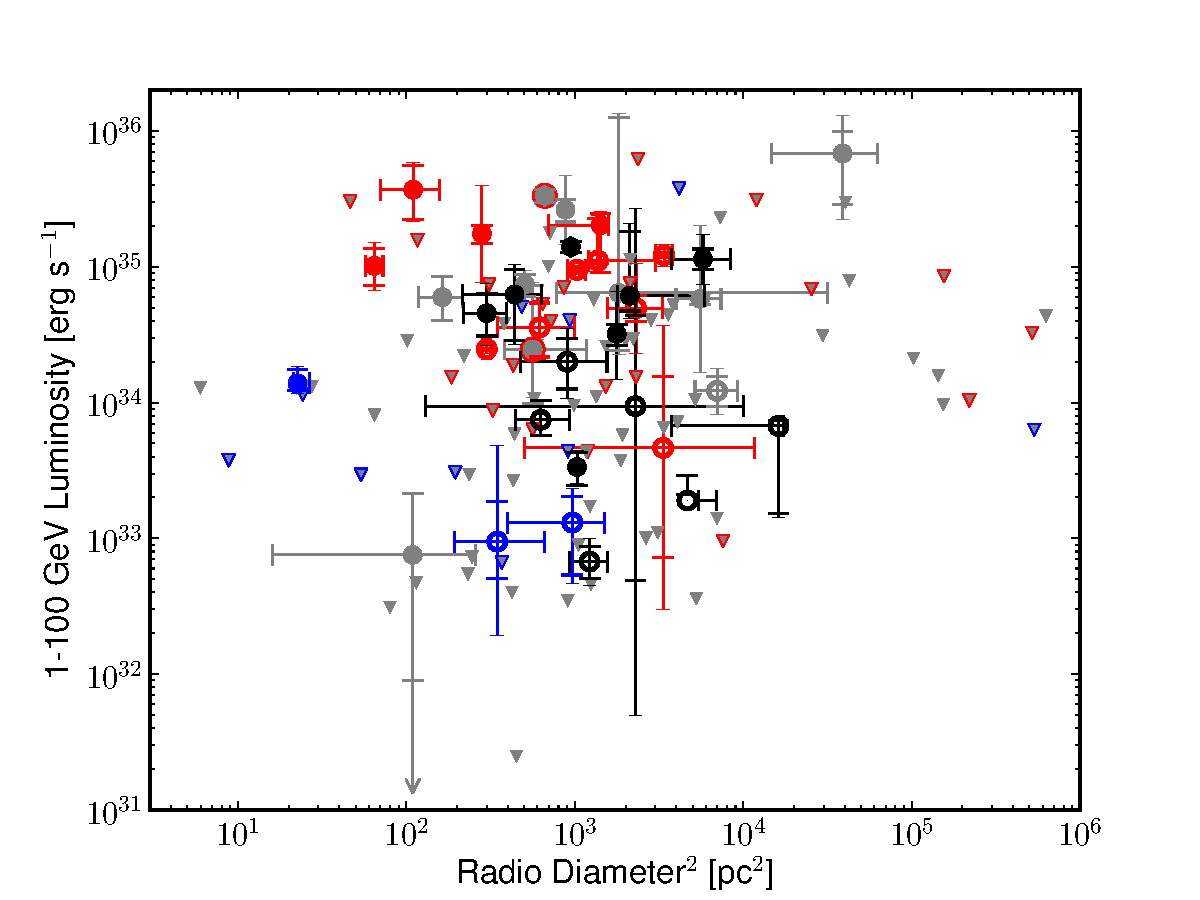
\includegraphics[width=1.0\columnwidth]{figures/lum_vs_dia2.pdf}
	\caption[$1-100$\,GeV luminosity vs. D$^2$ for SNRs with distance measurement.]{
		The $1-100$\,GeV luminosity is plotted against the square of the radio diameters in pc of those SNRs with known distances. Symbols, colors, and error bars are as in Figure~\ref{fig:GeVradioSize}.}
		\label{fig:LumDia}
\end{figure}

\jamie{didn't add anything about maximal CR energy content of all SNRs assuming purely hadronic emission, maybe don't need to}
\section{Conclusions}\label{snrcat:Conclusions}
In this Chapter, we have discussed the state of \gam{} observations of \snrs{} prior to the launch of \Fermi{}, and the unique role that the \lat{} plays in identifying \snrs{} and exploring \gam{} production mechanisms therein. We presented the new automated source addition and analysis method, \srcs{}, and its application to studying the population of \snrs{} emitting\gev{} \gam{}s, published in \cite{snrCat}. With this first \FermiLat{} SNR Catalog we have systematically characterized GeV emission in regions containing known radio SNRs, creating new methods to address issues associated with these typically complex regions. These include methods for systematically adding sources to a region and better estimating the systematic error due to choice of interstellar emission model (discussed in detail in)\cite{snrCat}). From this, we have determined characteristics of the GeV SNR population, down to our measurement limit, finding \nclassifiedsnrs~classified and \nmarginal~marginal candidates with a false identification limit of $< $\nninetyfivemockpercent  \citep{snrCat}. This GeV data provide a crucial context for the detailed modeling of individual SNRs. In combination with multiwavelength measurements, the GeV data now challenge simple, previously sufficient SNR emission models. Within the limits of existing multiwavelength data, our observations generally support previous findings of changes in spectral slope at or near TeV energies and a softening and brightening in the GeV range with age and effective age, yet we see indications that new candidates and new multiwavelength data may provide evidence of exceptions to this trend. % With uniformly measured data for all known SNRs, we also constrain SNRs' aggregate, maximal contribution to the population of Galactic CRs. With the GeV and other multiwavelength data, we find that the candidates and upper limits are generally within expectations if SNRs provide the majority of Galactic CRs and anticipate these limits will improve with both a larger GeV data set with better sensitivity, as will be provided by \FermiLat~Pass 8 data, and with more and better distance and density estimates.

\jamie{EGRET point source sensitivity is ${\rm \sim1x10^{-7}}\flux{}$
\url{http://fermi.gsfc.nasa.gov/science/instruments/table1-1.html} get this number from some paper instead?}

\jamie{Another pointlike assumption to speed things up is that the PSF doesn't vary too much with event incidence angle in individual bins. To ensure this even more, events with a reconstructed angle > 66.4deg (cos theta = 0.4) are removed (idk why this angle)}

\jamie{I did work for mock catalog, but it was really just running addsrcs centered on the mock positions}



\chapter{Extended Source Detection above 50 GeV: The 2FHL Catalog}
\label{chap:2FHL}

\section{Introduction}\label{2FHL:intro}
\jamie{give this a different title
    }
The \lat{} \citep{atwood09} on board the \Fermi{}
\gam{} space telescope has been surveying the whole sky since August 2008.
Its unprecedented sensitivity and localization accuracy allowed the detection
of over 3,000 point-like sources in  4\,years of data \citep[see the
third catalog of {\it Fermi}-LAT sources, 3FGL, ][]{3FGL}.
Typically, {\it Fermi}-LAT catalog studies are based on  source detection
and characterization in the whole 0.1\,GeV--100\,GeV energy band.
The larger photon statistics present at low energy, counterbalanced by
the LAT point-spread function (PSF) whose size decreases with energy,
yields an optimum sensitivity at a energies of a few GeV.
The {\it Fermi}-LAT catalogs are thus representative of the GeV sky
more than they are of the MeV or the sub-TeV sky.


The first {\it Fermi}-LAT catalog of hard sources, named 1FHL \citep{1FHL}, provided an unbiased census of the sky at energies from 10~GeV up to 500~GeV. %The comparison of 1FHL and 0.1--100\,GeV observations \citep[as provided in][]{2FGL} allowed us to uncover the presence of spectral breaks and to determine that  blazars of the BL Lacertae (BL Lac) type represented about 50\,\%of the entire source population { detected in that band}.
{ All-sky surveys at $\gamma$-ray energies} are instrumental for ground-based imaging atmospheric Cherenkov telescopes (IACTs) such as H.E.S.S., MAGIC, and VERITAS \citep[][respectively]{holder08,lorenz04,hinton04}
in order to find new sources because of their limited fields of view (FoV).


Recently, a new event-level  analysis (known as Pass 8) has been developed by the \emph{Fermi}-LAT collaboration \citep{atwood13b,atwood13}. Pass~8 significantly improves the LAT's background rejection, PSF, and effective area. All these  enhancements lead to a significant increase of the LAT sensitivity and its effective energy range, from below 100~MeV to beyond a few hundred GeV  \citep{atwood13b,atwood13}. These improvements are particularly significant above 50\,GeV, yielding an enhancement in the acceptance and PSF by a factor  between 1.2 and 2. 
It is interesting to note that, above 50\,GeV, both the PSF (governed mostly by the pitch of the tracker silicon strips and the spacing of the tracker planes, see Chapter \ref{FGST:LAT}) and the effective area of the LAT are only weakly dependent on energy and that the LAT 
operates, due to the (almost complete) absence of background, in the photon-limited regime.

We use 80\,months of Pass~8 data to produce a catalog of sources detected by the LAT at energies\footnote{Note the different energy range with respect to the 1FHL.} between 50\,GeV and 2\,TeV. This constitutes the second catalog of hard \lat{} sources, named \twofhl{}\jamie{add the if I haven't wrote 2fhl somewhere else yet}, which allows a thorough study of the properties of the whole sky in the sub-TeV domain. In this thesis, we present results published in \cite{2FHL}, exclusively focusing on the Galactic science analysis and results and eschew the extragalactic results to the published \twofhl{} paper \jamie{move this last sentence to the beginning and italicize?}.


%%%%%%%%%%%%%%%%%%%%%%%%%%%%%%%%%%%%%%%%%%%%%%%%%%%%%%%%%%%%%%%%
%
%         Analysis 
%
%%%%%%%%%%%%%%%%%%%%%%%%%%%%%%%%%%%%%%%%%%%%%%%%%%%%%%%%%%%%%%%%
\section{Analysis}
\label{sec:analysis}


%%%%%%%%%%%%%%%%%%%%%%%%%%%%%%%%%%%%%%%%%%%%%%%%%%%%%%%%%%%%%%%%
%
%         Detection
%
%%%%%%%%%%%%%%%%%%%%%%%%%%%%%%%%%%%%%%%%%%%%%%%%%%%%%%%%%%%%%%%%
% \subsection{\label{sec:sourceDetect}Data Selection and Source Detection}

\subsection{\label{sec:data_sel}Data Selection}


We use 80 months (from August 2008 to April 2015) of P8\_SOURCE 
photons with reconstructed energy in the 50\,GeV--2\,TeV range.
At these energies the LAT has an energy resolution of around 10--15\,\% (1\,$\sigma$).
Photons detected at zenith angles larger than 105$^{\circ}$ were excised
to limit the contamination from $\gamma$-rays generated by cosmic-ray
interactions in the upper layers of the atmosphere. Moreover, data were filtered
removing time periods when the instrument was not in sky-survey mode\footnote{This
    was achieved using the expression `(DATA\_QUAL$>$0)\&\&(LAT\_CONFIG==1)' in {\tt gtmktime}.}.
This leaves
approximately 61,000 photons detected across the entire  the sky. The count map
reported in Figure~\ref{fig:skymap} shows that the \lat{} observes
many point-like sources and
large scale diffuse emission in the direction of our Galaxy, some of which appears
coincident  with the so-called {\it Fermi} bubbles \citep{su10,lat_bubbles}.



\begin{figure*}[!ht]
    \begin{centering} 
        \includegraphics[width =\textwidth]{Figures/all-sky_countmap-Marco.eps}
        \caption{Adaptively smoothed count map in the 50\,GeV--2\,TeV band represented in Galactic coordinates and Hammer-Aitoff projection. The image has been smoothed with a Gaussian kernel whose size was varied to achieve a minimum signal-to-noise ratio under the kernel of 2. The color scale is logarithmic and the units are counts per (0.1\,deg)$^2$.
            \label{fig:skymap}}
    \end{centering}
\end{figure*}


\subsection{\label{2fhl:sourceDetect}Source Detection}


The first step of the source detection stage comprises the identification of source seeds, which are locations of potential sources whose significance is later tested through a maximum likelihood (ML) analysis. The seed detection method, described further in \cite{2FHL}, includes all the point sources detected in the 1FHL catalog. We note that  this seed list may include statistical fluctuations as well as real sources with a non-optimal position.

A full ML analysis is then performed in order to verify which,
among the seeds, are the reliable sources. 
The analysis is performed in 154 \rois{}, varying between 10$^{\circ}$ and 20$^{\circ}$ in radius, whose sizes and positions in the sky are optimized to cover all the seeds, ensuring that no more than 45 seeds are contained in a single \roi{}.
For each \roi{}, we build
a sky model that includes all the potential sources in the region
as well as the  Galactic and isotropic diffuse emissions\footnote{We~used~the~{\tt gll\_iem\_v06.fits}~and~{\tt iso\_P8R2\_SOURCE\_V6\_v06.txt}
    templates available at \\
    http://fermi.gsfc.nasa.gov/ssc/data/access/lat/BackgroundModels.html.}.
These models, which are defined only up to $\sim$600\,GeV and  $\sim$900\,GeV respectively, where extrapolated up to 2\,TeV.
The \roi{} models include also the extended sources present in the region (see Chapter \ref{2fhl:extended}).
The model is fit to the data via the unbinned ML algorithm provided
within the {\it Fermi} Science Tools\footnote{Available at 
    http://fermi.gsfc.nasa.gov/ssc/data/analysis/software/.} (version v9r34p3).

The spectrum of each source is modeled with a power law because
none of the sources is expected to show statistically
significant spectral
curvature detectable by the LAT in this energy band. 
Indeed, this was the case for the sources in the 1FHL catalog \citep{1FHL}.

The fit is performed iteratively in order to ensure convergence and 
to produce an optimal solution. It proceeds as follows:

\begin{enumerate}
    \item Complex ML fits require approximate knowledge of the 
    starting values of the parameters. For this reason the first
    step  aims to find those values  by fitting each single source separately 
    to determine approximate spectral parameters.
    Throughout the entire process, the parameters of the diffuse emission
    models are left free to vary.
    The significance of each source is evaluated using the test statistic  
    ${\rm TS}=2(\ln \mathcal{L}_1 - \ln \mathcal{L}_0)$, where $\mathcal{L}_0$ and $\mathcal{L}_1$
    are the likelihoods of the background (null hypothesis) and 
    the hypothesis being tested (\eg{} source plus background). 
    At each step in the procedure, marginal sources, those with TS $<$ 10, are removed from the model.
    Once the spectral parameters and significance of each source have
    been evaluated, a global fit for which all the parameters of the sources
    with a ${\rm TS}\geq 10$ are allowed to  vary is performed. 
    Then one more global fit is performed after removing all the sources that had ${\rm TS}< 10$ at the previous global fit.
    This step,
    as well as all the others, includes sources that
    are spatially extended (see Chapter \ref{2fhl:extended});
    
    \item In this second step, the positions of point-like sources, using the best-fit sky model
    derived at step 1, are optimized using the {\tt gtfindsrc} tool. This step
    is done iteratively as well by optimizing first the positions of the
    most significant sources found at step 1 and later  those of the fainter
    ones;
    
    \item The parameters and significances of sources are estimated again (as in step 1) using the best-fit source positions. This step produces the best-fit sky 
    model for any given \roi{}. 
    Seeds with $10\leq {\rm TS}<25$ are included in the model, but not reported in the final catalog;
    
    \item For each source we estimate the energy of the \hep{}
    that the fit attributes robustly  to the source model. This is done using the tool {\tt gtsrcprob} and selecting the HEP that has a probability $>85$\,\% to belong to the source;
    
    \item A  spectrum with three logarithmically spaced bins (boundaries of 50\,GeV, 171\,GeV, 585\,GeV, 2\,TeV) is generated for each source in the \roi{} that is detected with ${\rm TS}\geq 25$ and with the number of detected $\gamma$ rays (estimated by the likelihood, N$_{\rm pred}$) to be $\geq$3.
    
    
\end{enumerate}

The procedure described above achieves the detection of 360 sources (including
the extended sources discussed next in Chapter \ref{2fhl:extended}) 
with TS $\geq$ 25 and N$_{\rm pred}\geq3$ across the entire sky.
The number of seeds kept in the \roi{} models
with $10\leq{\rm TS}<25$ is 453, while 7 are seeds with ${\rm TS\geq}25$, but N$_{\rm pred}<3$.
\jamie{took out the monte carlo sims reasoning for Npred}
%We have performed seven Monte Carlo simulations of the $>$50\,GeV sky whose data have been analyzed like the real data (as detailed above). The  N$_{\rm pred}$ cut was introducedon the basis of these simulations to limit to $\lesssim$1\,\% the number of false positives in the final catalog. These simulations will be discussed in a forthcoming publication.

%%%%%%%%%%%%%%%%%%%%%%%%%%%%%%%%%%%%%%%%%%%%%%%%%%%%%%%%%%%%%%%%
%
%         Extended Sources
%
%%%%%%%%%%%%%%%%%%%%%%%%%%%%%%%%%%%%%%%%%%%%%%%%%%%%%%%%%%%%%%%%
\section{Search for Spatially-Extended Sources}
\label{2fhl:extended}


Preliminary runs of the source detection method described in Chapter \ref{2fhl:sourceDetect} detected clusters of point sources in the Galactic plane, which were suggestive of spatially extended sources. It is also possible that clusters of seed sources, each with sub-detection-threshold significance, could be detected as a significant extended source. 
Not modeling extended $\gamma$-ray emission as such can lead to inaccurate measurements of spectral and spatial properties of both the extended source and neighboring point sources, particularly in the Galactic plane \citep{Lande12}. Most of the TeV sources in the Galactic plane are spatially
extended  \citep{carrigan2013, ong2013}, 
so to clearly connect LAT detections spectrally to these sources, extension detection and characterization is important.
In the following, we distinguish between sources whose extension
have been previously determined with {\it Fermi}-LAT and
new extended sources that are reported for the first time
in a \lat{} catalog. The details of all significantly
detected extended sources are reported  in Chapter \ref{2fhl:ESresults}. 

%%%%%%%%%%%%%%%%%%%%%%%%%%%%%%%%%%%%%%%%%%%%%%%%%%%%%%%%%%%%%%%%
%
%         Extended Sources in 3FGL
%
%%%%%%%%%%%%%%%%%%%%%%%%%%%%%%%%%%%%%%%%%%%%%%%%%%%%%%%%%%%%%%%%

\subsection{\label{2fhl:3FGL_ES}Extended Sources Previously Detected by the LAT}
We explicitly modeled sources as spatially extended when a previous, dedicated, analysis found the source to be resolved by the LAT.
The 25 extended sources reported in 3FGL were included in our model using the spatial templates derived in the individual source studies \citep[see references in ][]{3FGL}. Refitting the positions and extensions of the 3FGL extended sources in this energy range is beyond the scope of this work.

Of the 25 3FGL extended sources, 19 are significantly detected here above the detection threshold (${\rm TS}\geq25$). Only 6 sources are not detected and, since all have  ${\rm TS<10}$, are removed from the sky model (see Chapter \ref{2fhl:ESresults} for details).

One extended LAT source has had a dedicated analysis published since the release of the 3FGL catalog. \cite{HESSLATW41} reported joint H.E.S.S. and LAT observations of the \vhe{} source HESS~J1834-087. This source is coincident with \snr{} W41 and was detected  as spatially extended in a wide energy range spanning 1.8\,GeV to 30\,TeV. In this paper, we employ the spatial model for the GeV emission determined in \cite{HESSLATW41}, leading to a significant detection of this source.


%%%%%%%%%%%%%%%%%%%%%%%%%%%%%%%%%%%%%%%%%%%%%%%%%%%%%%%%%%%%%%%%
%
%         Extended Sources not in 3FGL
%
%%%%%%%%%%%%%%%%%%%%%%%%%%%%%%%%%%%%%%%%%%%%%%%%%%%%%%%%%%%%%%%%
\subsection{\label{2fhl:newES}Newly Detected Extended Sources} %\jamie{should this be changed to something like ``Newly Detected Extended Sources" since W41 is now included in the previous section and is not a 3FGL source?}

In addition to modeling the extended sources mentioned in Chapter \ref{2fhl:3FGL_ES}, we performed a blind search of the Galactic plane  (\blat) to identify potential extended sources not included in previously published works. Our analysis pipeline is similar to that used in \cite{snrCat} (described in detail in Chapter \ref{snrcat:ptlkt}), with some modifications tailored to searching for multiple extended sources in an \roi{}. The pipeline employed the {\tt pointlike} binned maximum likelihood package \citep{Kerr10}, in particular utilizing the extended source fitting tools validated by \cite{Lande12} to simultaneously fit the position, extension, and spectra of sources in our \rois{}. We used the \srcs{} method (developed for the \snrcat{} and described in Chapter \ref{snrcat:AddSrcs}) to characterize potentially extended sources across the Galactic plane. We detail how it was applied to the \twofhl{} study below.

We created 72 \roi{}s of radius ${\rm 10^{\circ}}$, centered on ${\rm b = 0^{\circ}}$ with neighboring \roi{}s overlapping and separated by ${\rm 5^{\circ}}$ in Galactic longitude.  Our initial model of the $\gamma$-ray emission in each \roi{} consisted solely of the Galactic diffuse (allowing just the normalization to be fit) and isotropic emission models (fixing the normalization), with no other sources in the \roi{}. Emission in the \roi{}s was further characterized by iteratively adding sources and fitting their spectral parameters (normalization and spectral index) in a ${\rm 14^{\circ}}\times{\rm 14^{\circ}}$ region. 

A TS map, that included all significant sources found previously, made up of ${\rm 0.1^{\circ}}\times{\rm 0.1^{\circ}}$ bins across the \roi{}, was created at each iteration and a small radius (${\rm 0.1^{\circ}}$) uniform disk, with a power-law spectrum was placed at the position of the peak TS pixel. The spectra of any newly added sources, as well as the position, extension, and spectral parameters of the disk were then fit. If $\rm TS_{ext} \geq 16$, where  ${\rm TS_{ext} = 2~log(\mathcal{L}_{ext} / \mathcal{L}_{ps})}$ \citep[\ie{} twice the log-likelihood ratio of an extended to a point source,][]{Lande12}, then the disk was kept in the model. For $\rm TS_{ext} < 16$, the extended source was replaced by a point source with a power-law spectral model. For the point-source replacement case, spectral parameters of sources in the \roi{} were fit and the position of the new point source was optimized. Finally, the spatial parameters of any previously added extended sources were refit iteratively before creating a new TS map and repeating the process. We stopped adding sources when the peak TS was less than 16 for two successive sources. 

{ To assess the impact of fitting extended sources when starting with an \roi{} devoid of sources, a crosscheck analysis (also using {\tt pointlike}) was performed across the Galactic plane. We included 3FGL point and extended sources, the Galactic diffuse and isotropic emission, and pulsars from the \twopc{} catalog \citep{2PC} (as well as from 3FGL) in the preliminary source model for each region. Sources were iteratively added to account for residual emission and both these residual sources and 3FGL  sources were tested for extension. Remarkably, this alternative analysis converges (\ie{ spectral and spatial parameters for the detected extended sources are compatible in both analyses) to the initially source-devoid analysis for nearly all detected extended sources.
}

Extended sources detected in the analysis described in this chapter for which the position and extension  were compatible with those found by the crosscheck were included in the \roi{} model at step 1 of the full ML analysis detailed in Chapter \ref{2fhl:sourceDetect}. Seed point sources interior to the extended sources were removed prior to the ML fit. Since any source that had ${\rm TS_{ext} < 16}$ reverted to a point source model, \srcs{} characterized  both extended and point-like emission in each \roi{}. While the extended source results were passed into the ML fit, the point source results derived with \ptlike{} were not included. Despite their non-inclusion, the point source results were cross-checked against the final results of the ML procedure  to ensure there were no glaring inconsistencies, of which none were found.

To address the ambiguity between detecting a source as spatially extended as opposed to a combination of point sources, we utilized the algorithm detailed in \cite{Lande12} to simultaneously fit the spectra and positions of two nearby point sources. ${\rm TS_{2pts}}$ is defined as twice the log of the ratio of the likelihood for the region containing two point sources to the same region with a single point source, ${\rm TS_{2pts} = 2log(\like{}_{2pts} /\like{}_{ps}})$. We only consider a source to be extended if ${\rm TS_{ext} > TS_{2pts}}$. Since the extended and two point source hypotheses are not nested models, a likelihood-ratio test cannot be used to quantitatively compare ${\rm TS_{2pts}}$ with ${\rm TS_{ext}}$ to determine which is the more significant model. Despite this, \cite{Lande12} showed through Monte Carlo simulations that comparing the two likelihood ratios is a strong test for determining if the detected emission truly arises from two point sources, and that it is unlikely to incorrectly favor the two-point hypotheses if a sources is extended. We only consider a source to be extended if $\rm TS_{ext}~ >$ $\rm TS_{2pts}$. 

Our blind search of the Galactic plane allowed us to find 5 sources not previously detected as extended by {\it Fermi}-LAT.  Further details on these sources are presented in Chapter \ref{2fhl:ESresults}.



%%%%%%%%%%%%%%%%%%%%%%%%%%%%%%%%%%%%%%%%%%%%%%%%%%%%%%%%%%%%%%%%
%
%         Results
%
%%%%%%%%%%%%%%%%%%%%%%%%%%%%%%%%%%%%%%%%%%%%%%%%%%%%%%%%%%%%%%%%

\section{The 2FHL Catalog}
\label{2fhl:results}
\begin{figure*}[!ht]
	\centering
	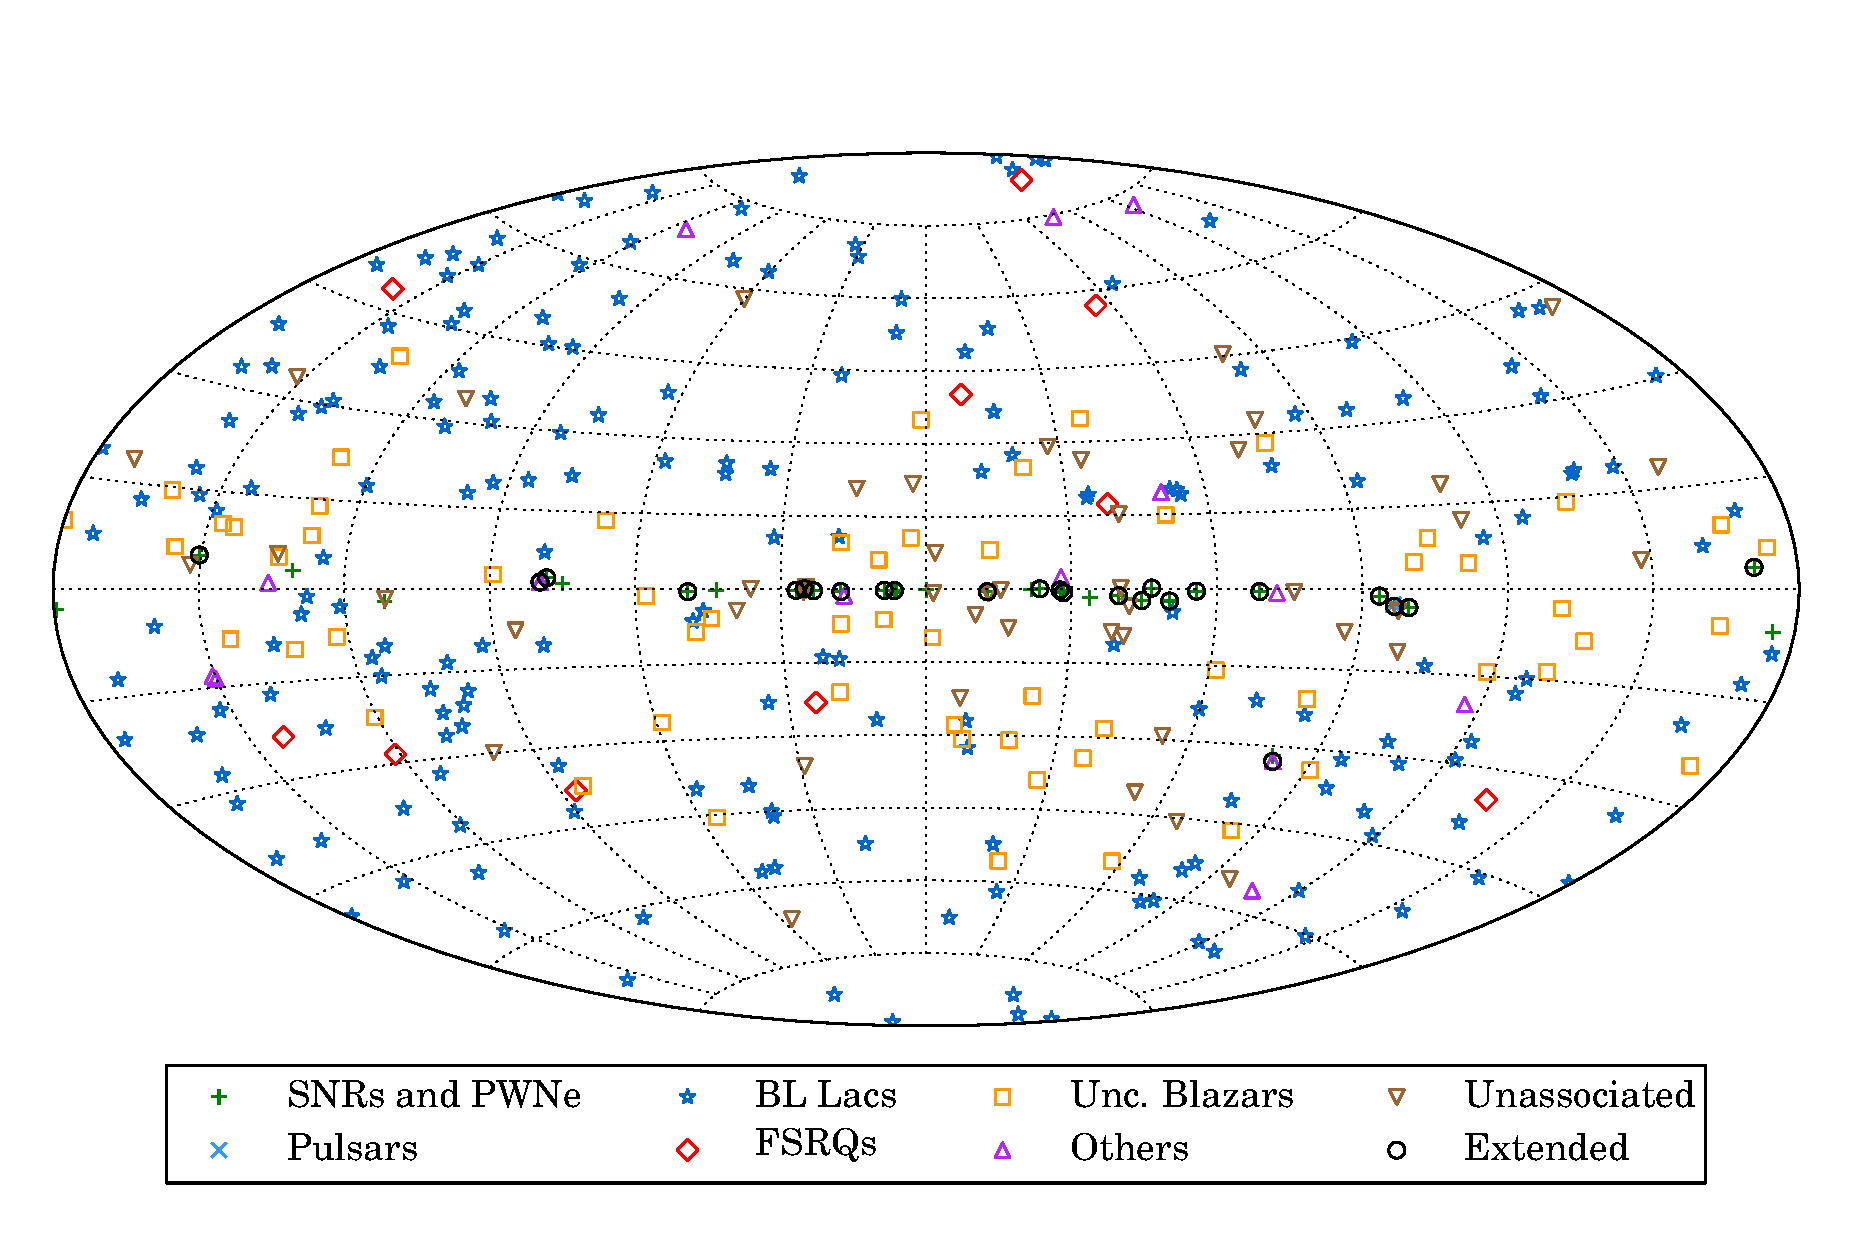
\includegraphics[width=\textwidth]{Figures/all-sky_assoc.eps} 
	\caption{Sky map, in Galactic coordinates and Hammer-Aitoff projection,
		showing the sources in the 2FHL catalog classified by their most likely association. 
		\label{fig:all_sky}}
\end{figure*}
The 2FHL catalog \footnote{FITS catalog can be found at \url{http://fermi.gsfc.nasa.gov/ssc/data/access/lat/2FHL/}} includes 360 sources detected over the whole sky, each with a likelihood test statistic of ${\rm TS}\geq 25$ and number of associated photons, $N_{\rm pred}\geq 3$. 
The source association procedure (detailed in \cite{2FHL}) finds that 75\% of the sources in the catalog (274 sources) are extragalactic\footnote{This includes N~157B, an extragalactic \pwn{}.}, 11\% (38 sources) are of Galactic nature, and 13\% (48 sources) are unassociated (or associated with a TeV source of unknown nature). The unassociated sources are divided between 23 sources located at $|b|<10^{\circ}$, and 25 sources at $|b|\geq 10^{\circ}$. Therefore the fraction of extragalactic sources in the sample is likely larger than 80\,\%. The number of 2FHL sources that have not been reported in 3FGL is 57, 47 of which have not been previously reported in any \lat{} catalog nor in the TeVCat\footnote{\url{http://tevcat.uchicago.edu/}} catalog of \tev{} detected sources, and are thus new $\gamma$-ray sources. % The results of the association procedures are summarized in Table~\ref{tab:class}.
 Figure~\ref{fig:all_sky} shows the location of 2FHL sources, color-coded according to their source class.\jamie{left out the assoc table}

%% Table listing the source classes and their numbers
\begin{deluxetable}{lcr}
\setlength{\tabcolsep}{0.04in}
\tablewidth{0pt}
\tabletypesize{\small}
\tcap{2FHL Source Classes \label{tab:class}}
\tablehead{
\colhead{Description} & 
\multicolumn{2}{c}{Associated} \\
& 
\colhead{Designator} &
\colhead{Number}
}
\startdata
Pulsar & psr & 1 \\
Pulsar wind nebula & pwn & 14 \\
Supernova remnant & snr & 16 \\
Supernova remnant / Pulsar wind nebula & spp & 4 \\
High-mass binary & hmb & 2 \\
Binary & bin & 1 \\
Star-forming region & sfr & 1 \\
BL Lac type of blazar & bll & 180 \\
BL Lac type of blazar with prominent galaxy emission & bll-g & 13 \\
FSRQ type of blazar & fsrq & 10 \\
Non-blazar active galaxy & agn & 2 \\ 
Radio galaxy & rdg & 4 \\
Radio galaxy / BL Lac  & rdg/bll & 2 \\
Blazar candidate of uncertain type I & bcu I & 7 \\
Blazar candidate of uncertain type II & bcu II & 34 \\ 
Blazar candidate of uncertain type III & bcu III & 19 \\  
Normal galaxy (or part) & gal & 1 \\
Galaxy cluster & galclu & 1 \\
Total associated & \nodata & 312 \\
%\hline
Unassociated & \nodata & 48 \\ 
\hline
Total in 2FHL & \nodata & 360 \\ 

\enddata
\tablecomments{The designation `spp' indicates potential association with SNR or PWN.
The `bcu I', `bcu II', and `bcu III' classes are derived from 3LAC  and describe the increasing lack of multiwavelength information to classify  the source as a blazar \citep[see ][for more details]{3LAC}. The designation `bll-g' is adapted from the BZCAT \citep{bzcat5} and indicates a blazar whose SED has a significant contribution from the host galaxy.}
\end{deluxetable}



%%%%%%%%%%%%%%%%%%%%%%%%%%%%%%%%%%%%%%%%%%%%%%%%%%%%%%%%%%%%%%%%
%
%         General Results
%
%%%%%%%%%%%%%%%%%%%%%%%%%%%%%%%%%%%%%%%%%%%%%%%%%%%%%%%%%%%%%%%%
\subsection{General Characteristics of 2FHL Sources}\label{2fhl:General}

The 2FHL sources have $>$ 50\,GeV fluxes ranging from
$\sim$$8\times 10^{-12}$~ph~cm$^{-2}$~s$^{-1}$ to $\sim$$1.3\times 10^{-9}$~ph~cm$^{-2}$~s$^{-1}$
with a median flux of  $2.0\times 10^{-11}$~ph~cm$^{-2}$~s$^{-1}$
and a median spectral index of 2.83. The index uncertainty increases rapidly with the spectral index (\eg{} the uncertainty is about
$\pm 0.5$ for sources with $\Gamma=2$ whereas it is 
$\pm 2$ for sources with $\Gamma=5$).
Half of the sources are localized to better than
1.7$'$ radius at 68\,\% confidence. 
\jamie{don't include flux vs index stuff}
%Figure~\ref{fig:index_vs_flux} plots the spectral index versus the photon flux for sources associated with extragalactic sources or located at \blot (the extragalactic sample), Galactic sources, and unassociated sources. Figure~\ref{fig:index_vs_flux} shows that there is no visible dependence of the sensitivity (i.e. minimum dethighlighting that the sensitivity for source detection becomes { worse} in the plane of the Galaxy.} 
The distributions of spectral indices and the highest photon energy reported in Figure~\ref{fig:hist_index} show that extragalactic sources tend to have larger photon indices (median of 3.13) than Galactic sources (median of 2.10).   Because of the harder spectra, Galactic sources tend to have higher-energy HEPs than those of extragalactic sources
as shown as well in Figure~\ref{fig:hist_index}.
It is interesting to note that unassociated sources have a median index of 2.22 (2.00 for  sources at \blat and 2.96 for those at \blot), showing that a fraction (see Chapter \ref{2fhl:GalPop}) of unassociated sources are likely of Galactic origin. 

Building a spectral energy distribution (SED) represents a powerful way to discriminate or infer the nature of a source. By combining the spectral data from the 3FGL, 1FHL, and 2FHL catalogs, it becomes possible to measure the SEDs
of sources over four decades in energy. Although these catalogs rely on different exposures and  most $\gamma$-ray sources are variable, these data allow us to characterize the high-energy peak of their broadband SEDs. The SEDs of a few notable sources will be shown in the next sections.

%%%%%%%%%%%%%%%%%%%%%%%%%%%%%%%%%%%%%%%%%%%%%%%%%%%%%%%%%%%%%%%%
%
%         Galactic Science
%
%%%%%%%%%%%%%%%%%%%%%%%%%%%%%%%%%%%%%%%%%%%%%%%%%%%%%%%%%%%%%%%%

\subsection{The 2FHL Galactic Source Population}\label{2fhl:GalPop}


The narrow PSF core (about $0.1^{\circ}$) and moderate Galactic diffuse emission (in comparison with the $>100$\,MeV band) allows the LAT to characterize and study well the emission of sources in the plane of our Galaxy above 50\,GeV. Within $|b|<10^{\circ}$, \lat{} has detected 103 sources.
Of those, 38 sources are associated with Galactic sources, 42 with blazars, 14 are unassociated and 9 are associated with other $\gamma$-ray sources
whose origin is not known (see below).
Figure~\ref{fig:gp1} shows cut-outs of the Galactic plane with all detected sources labeled.

\begin{figure*}[!ht]
    \begin{centering}
        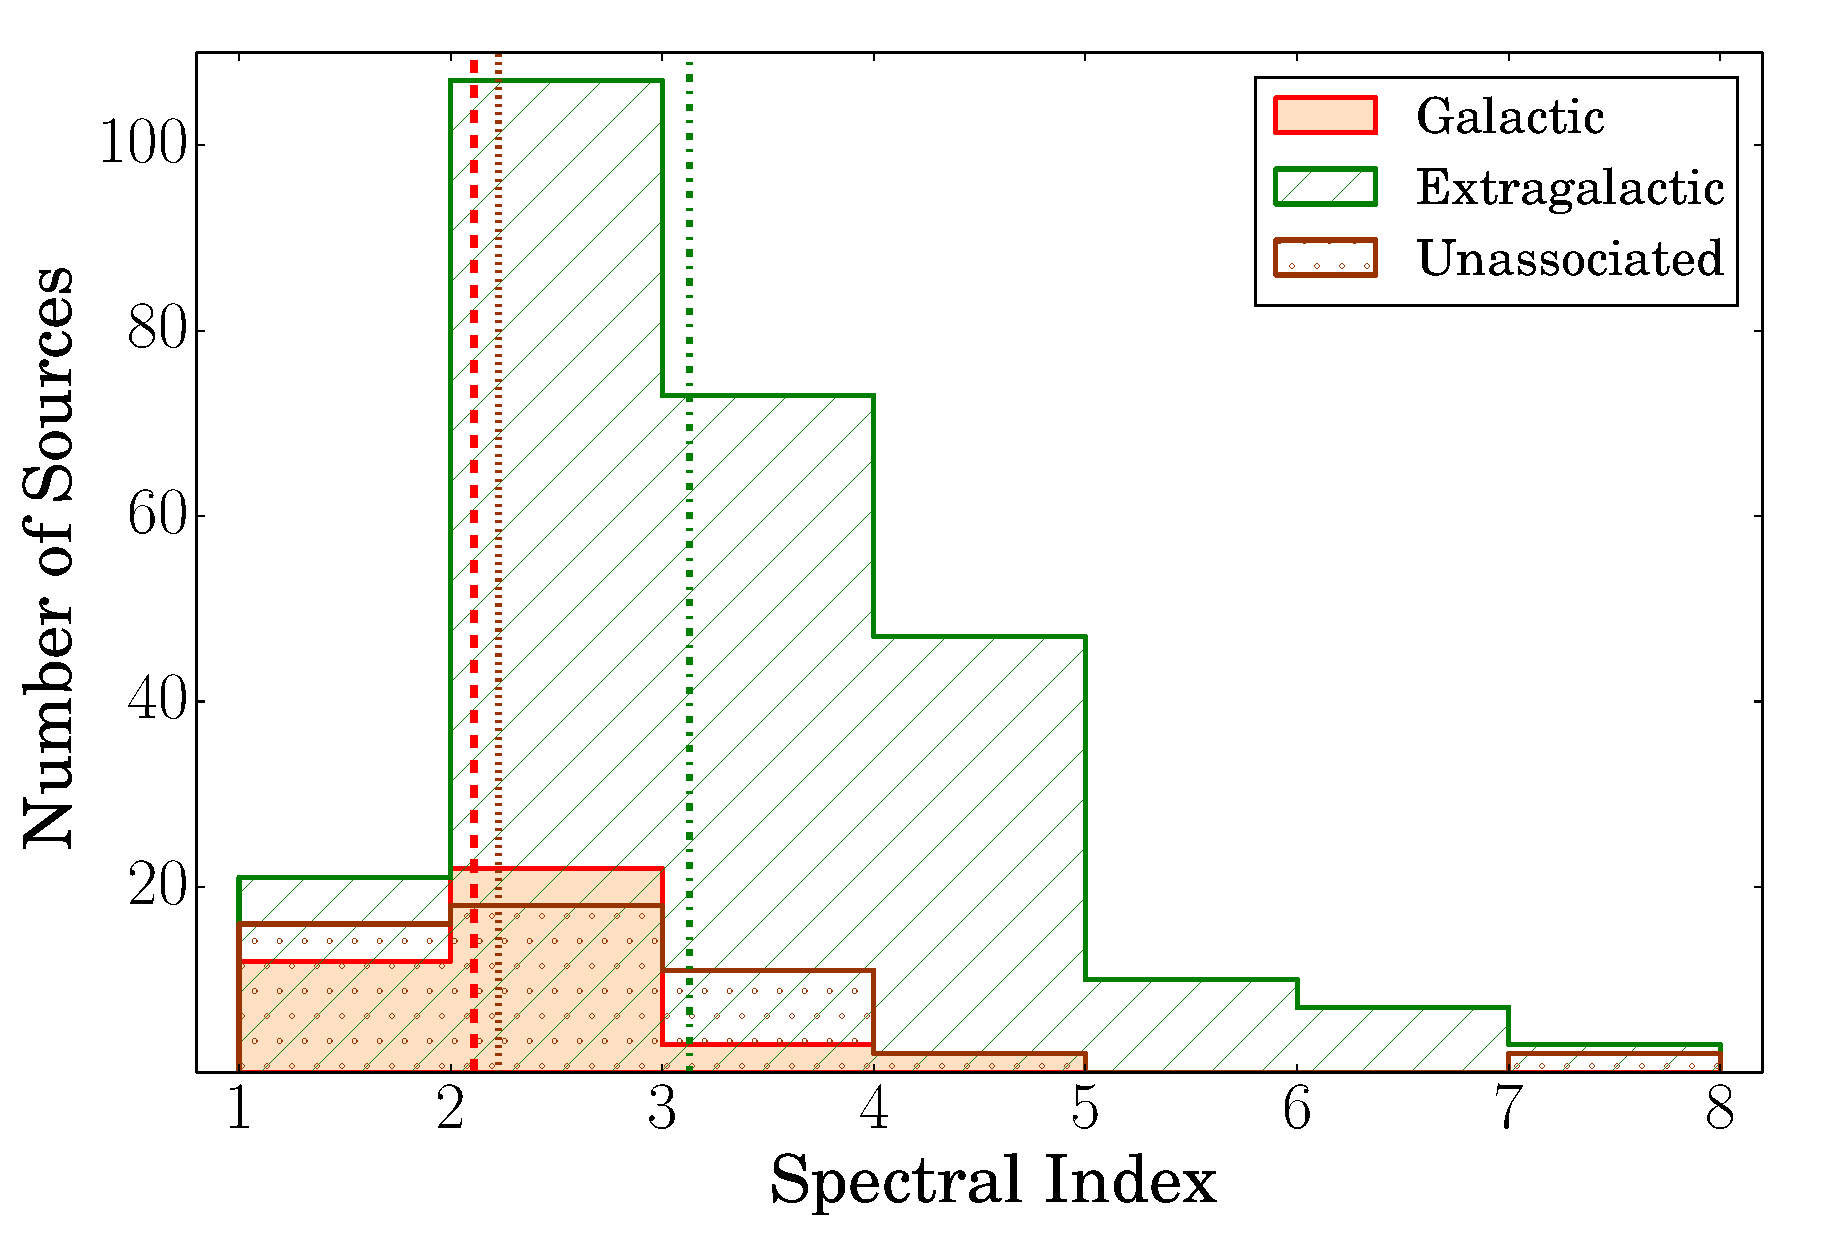
\includegraphics[width=0.9\columnwidth]{Figures/hist_index-new.eps}
         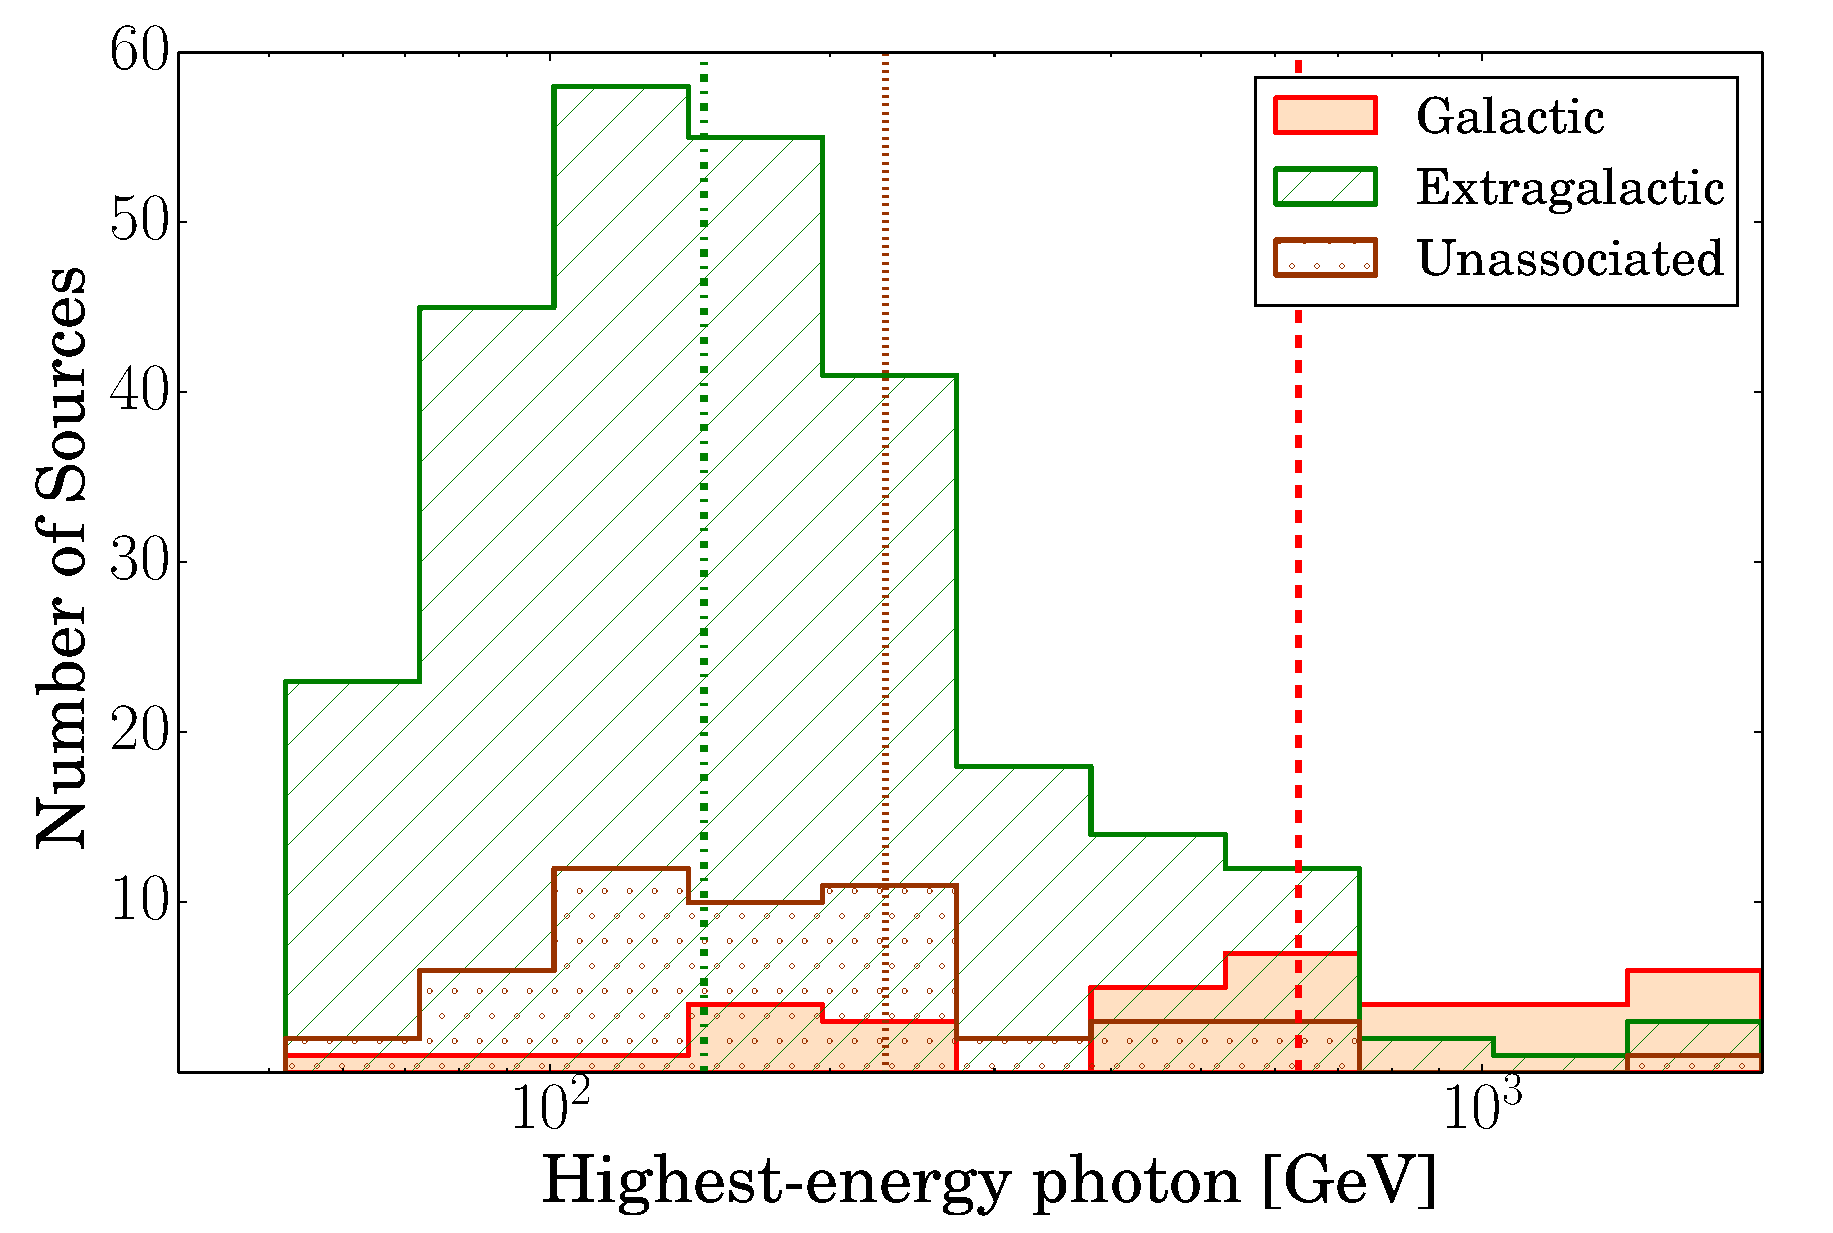
\includegraphics[width=0.9\columnwidth]{Figures/hist_hep-new.eps} 
        \caption{Distribution of the spectral indices ({\it top panel}) and highest photon energy ({\it bottom panel}) of the Galactic sources (orange), extragalactic sources (green slash), and unassociated sources (brown dotted). The medians of the distributions are plotted with dashed, dash-dotted, and dotted vertical lines, respectively. Both plots show that a distinct population of hard-spectrum sources is of Galactic origin.
            \label{fig:hist_index}}
    \end{centering}
\end{figure*}

Among the 38 Galactic sources, 16 are spatially coincident with SNRs, 13 are coincident with PWNe, 4 are associated with PWN/SNR complexes
and the other 5 sources are X-ray binaries (3), one pulsar (PSR~J0835$-$4510)
and the Cygnus Cocoon.
It is clear that the majority of Galactic sources detected above 50\,GeV
are associated with objects at the final stage of stellar evolution.

\begin{figure*}[!ht]
    \begin{center}
        \begin{tabular}{ll}
            % original scale=0.4
                    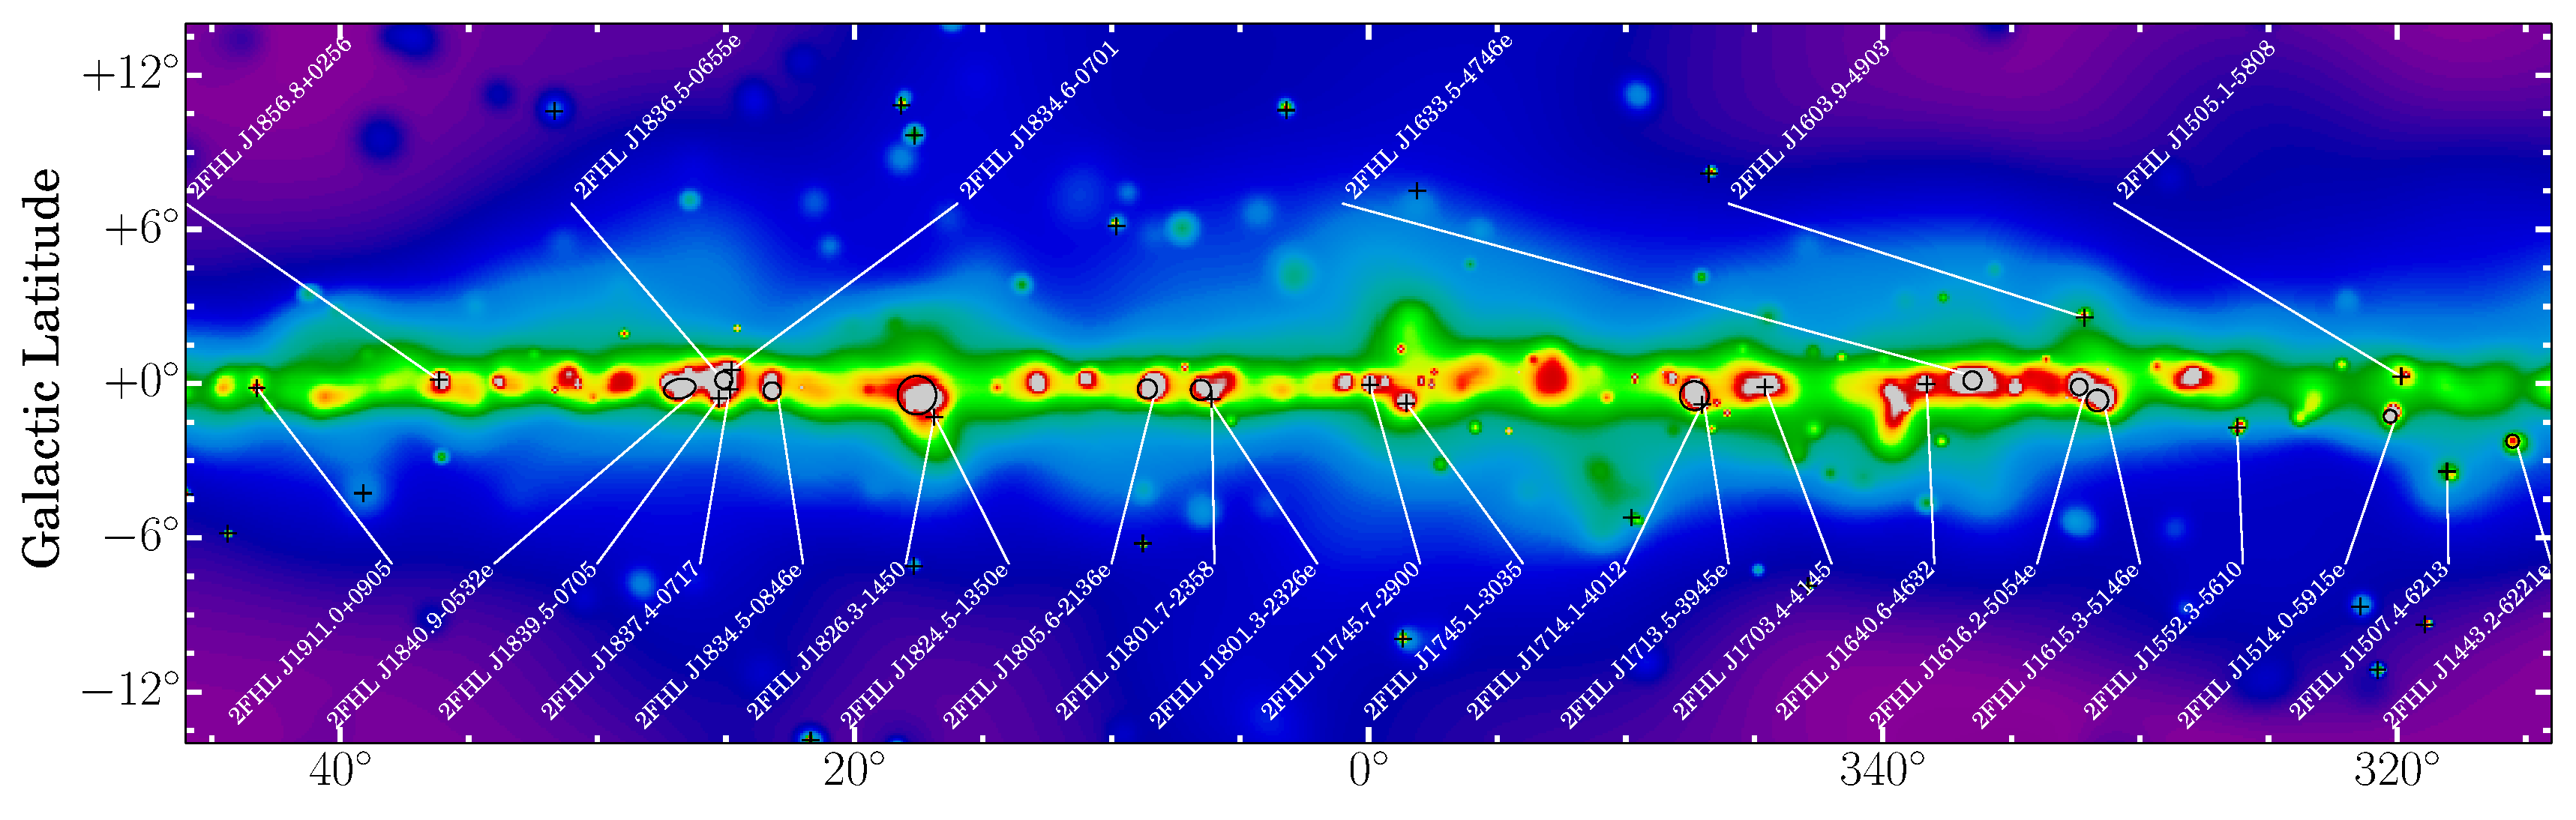
\includegraphics[angle=90,scale=.3]{Figures/Galactic_plane_CAR_1of4_sqrt_spectral_2FHL.eps}&
                    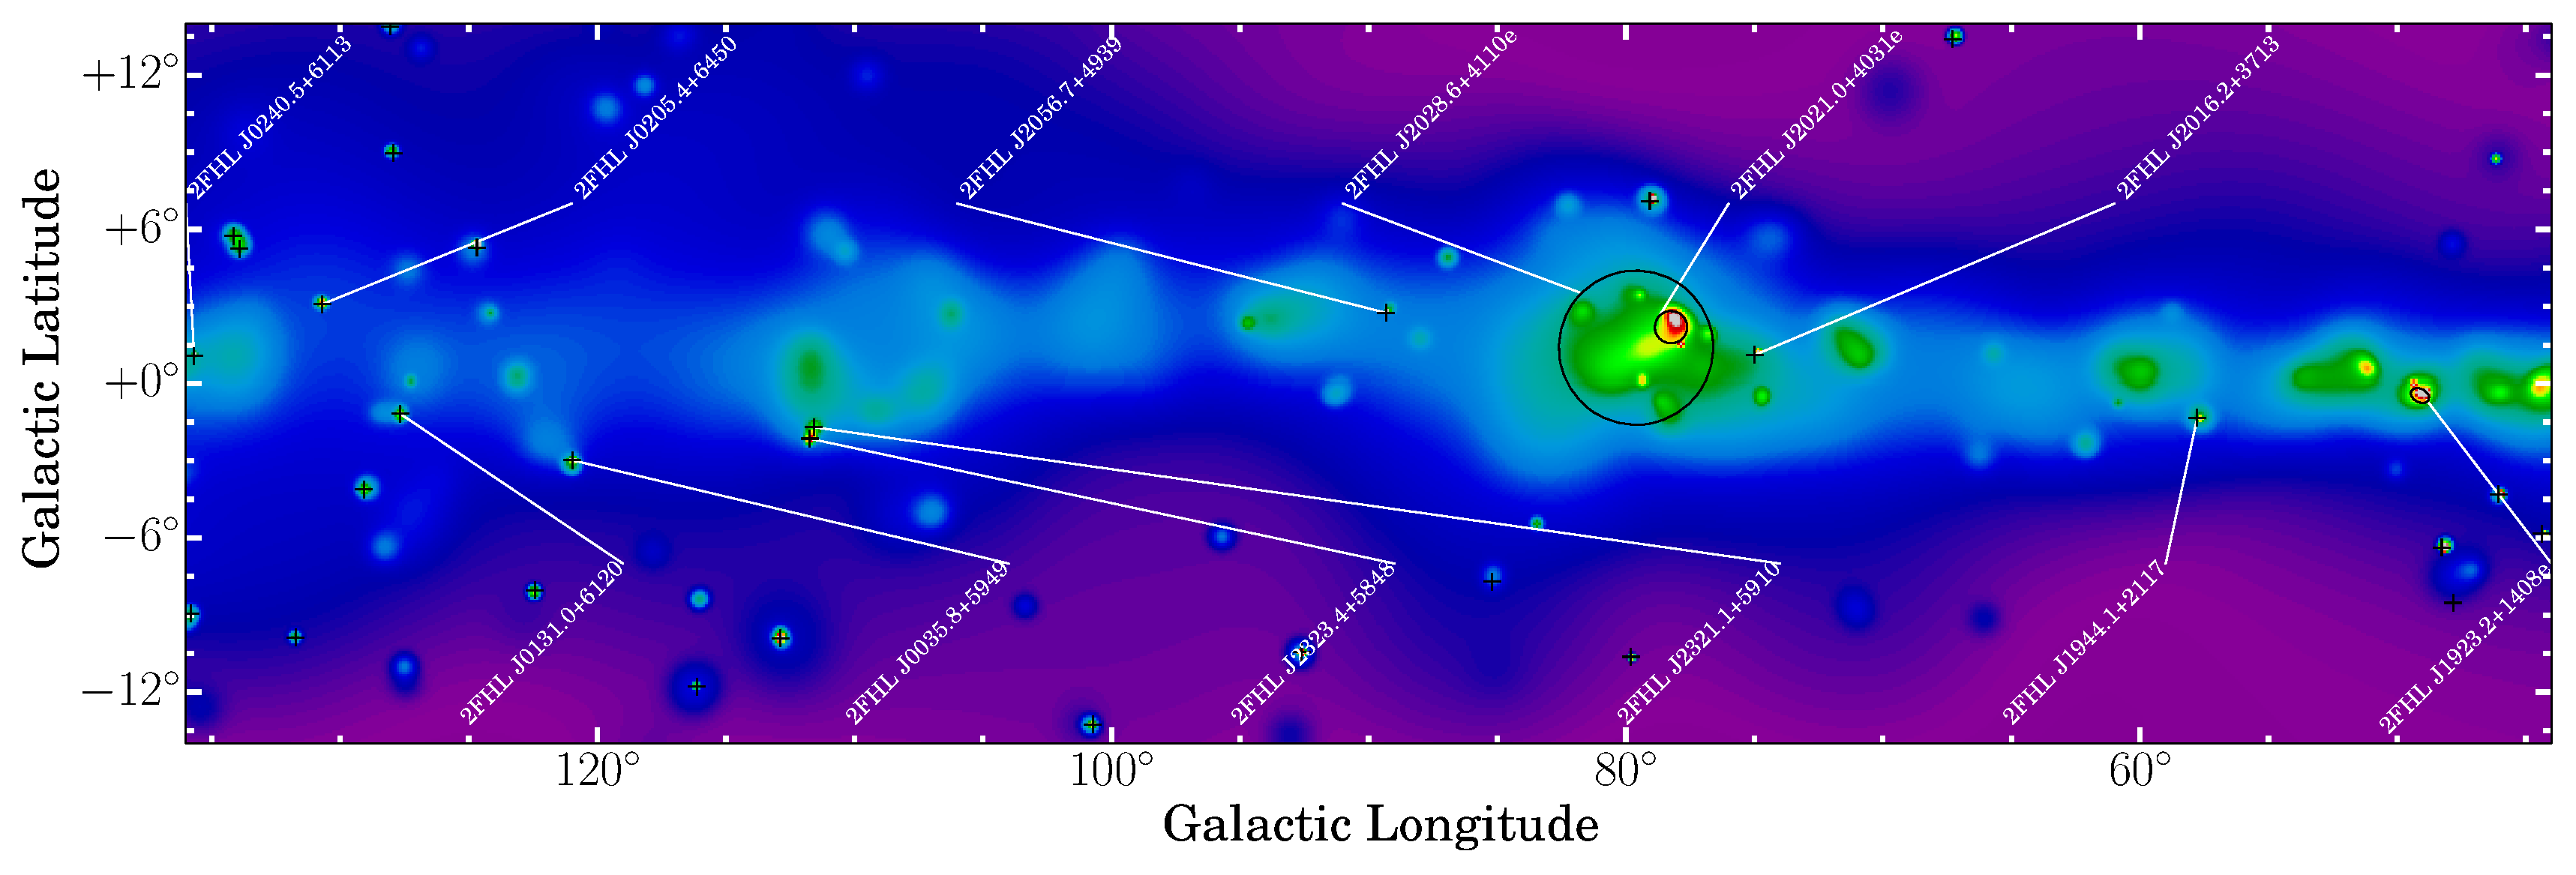
\includegraphics[angle=90,scale=.3]{Figures/Galactic_plane_CAR_2of4_sqrt_spectral_2FHL.eps}\\
            %\includegraphics[angle=90,scale=.3]{f5a.eps}&
            %\includegraphics[angle=90,scale=.3]{f5b.eps}\\
            
            
        \end{tabular}
    \end{center}
    \caption{Adaptively smoothed count map showing the whole Galactic plane $0^{\circ}\leq l\leq 360^{\circ}$ at Galactic latitudes $-14^{\circ} \leq b\leq 14^{\circ}$ divided in four  panels. The panels are centered at $l=0^{\circ}$, $90^{\circ}$, $180^{\circ}$ and $270^{\circ}$, respectively. Detected point sources are marked with a cross whereas extended sources are indicated with  their extensions. Only sources located at $-4^{\circ} \leq b\leq 4^{\circ}$ are explicitly named, plus the Crab Nebula.
        \label{fig:gp1}}
\end{figure*}


\begin{figure*}[!ht]
    \begin{center}
        \begin{tabular}{ll}
                    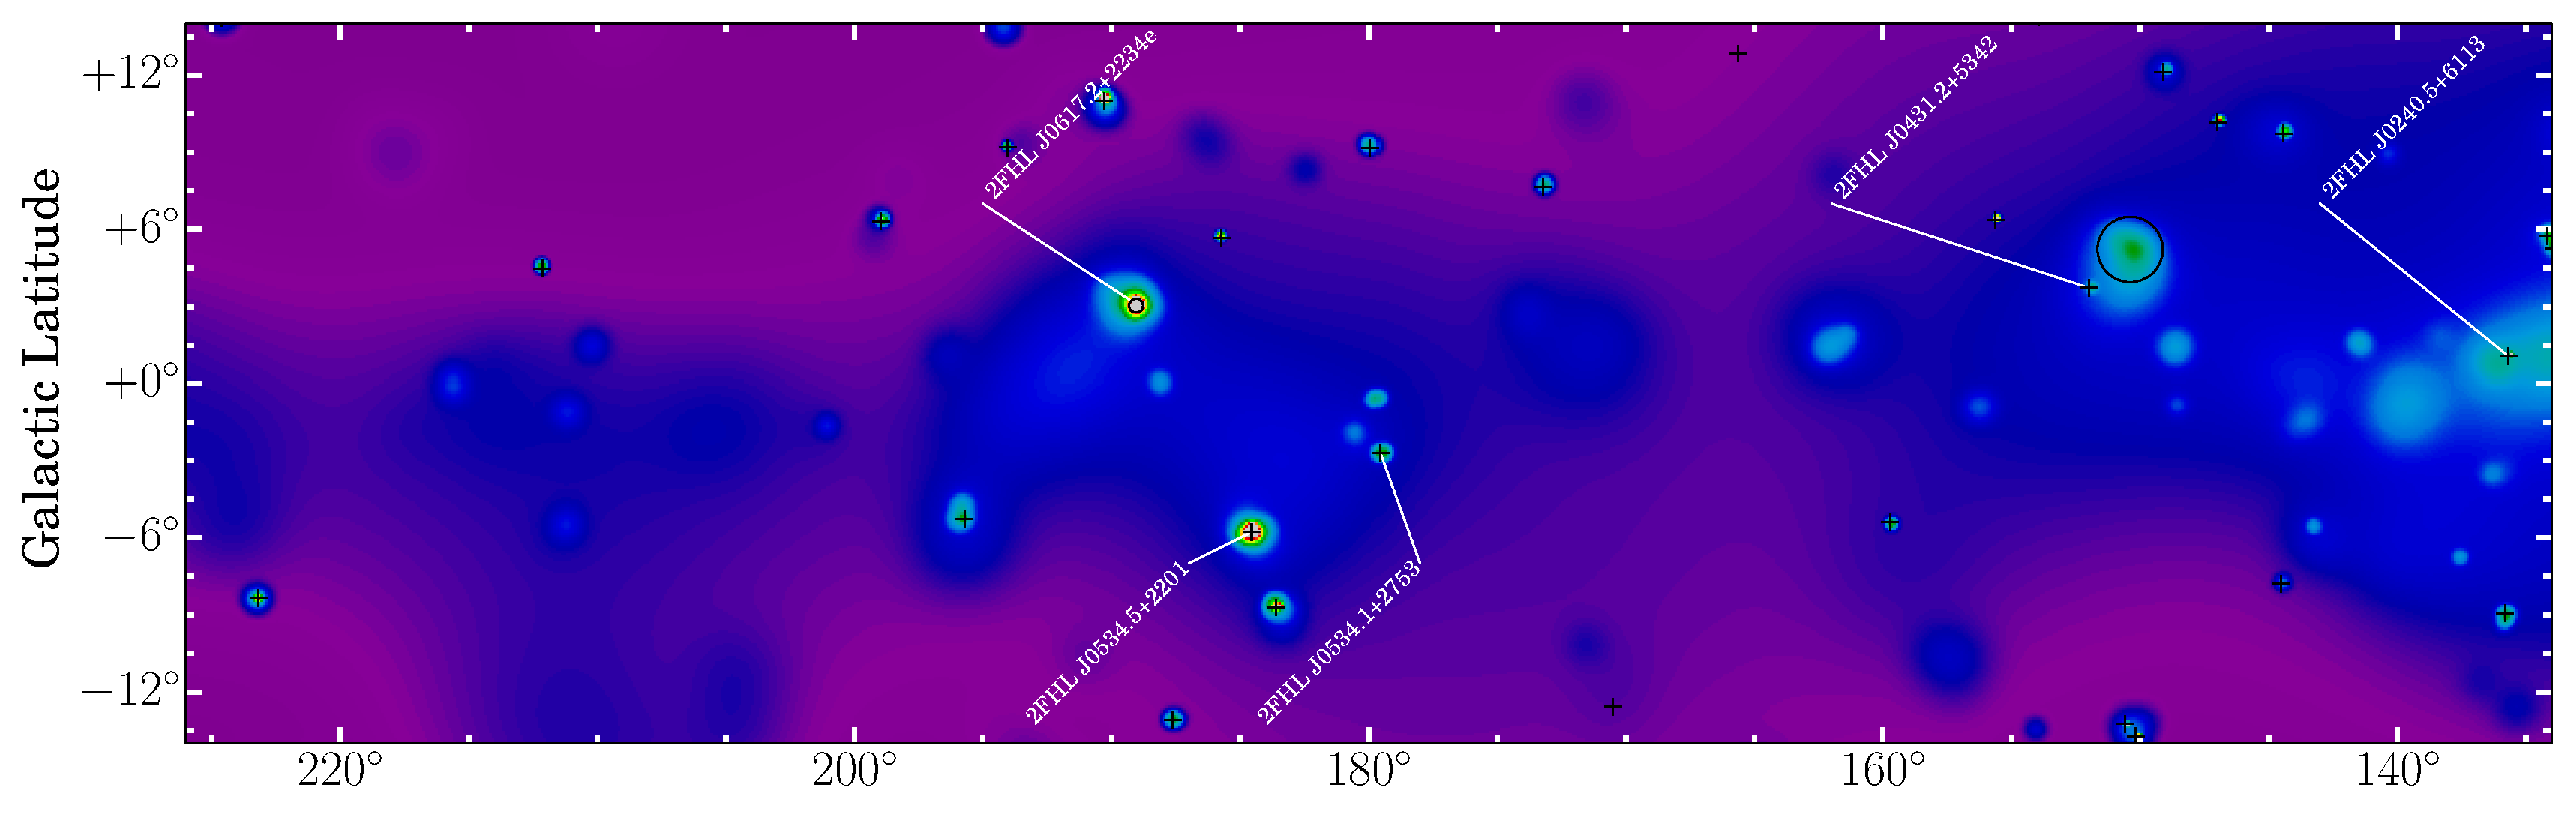
\includegraphics[angle=90,scale=.3]{Figures/Galactic_plane_CAR_3of4_sqrt_spectral_2FHL.eps}&
                    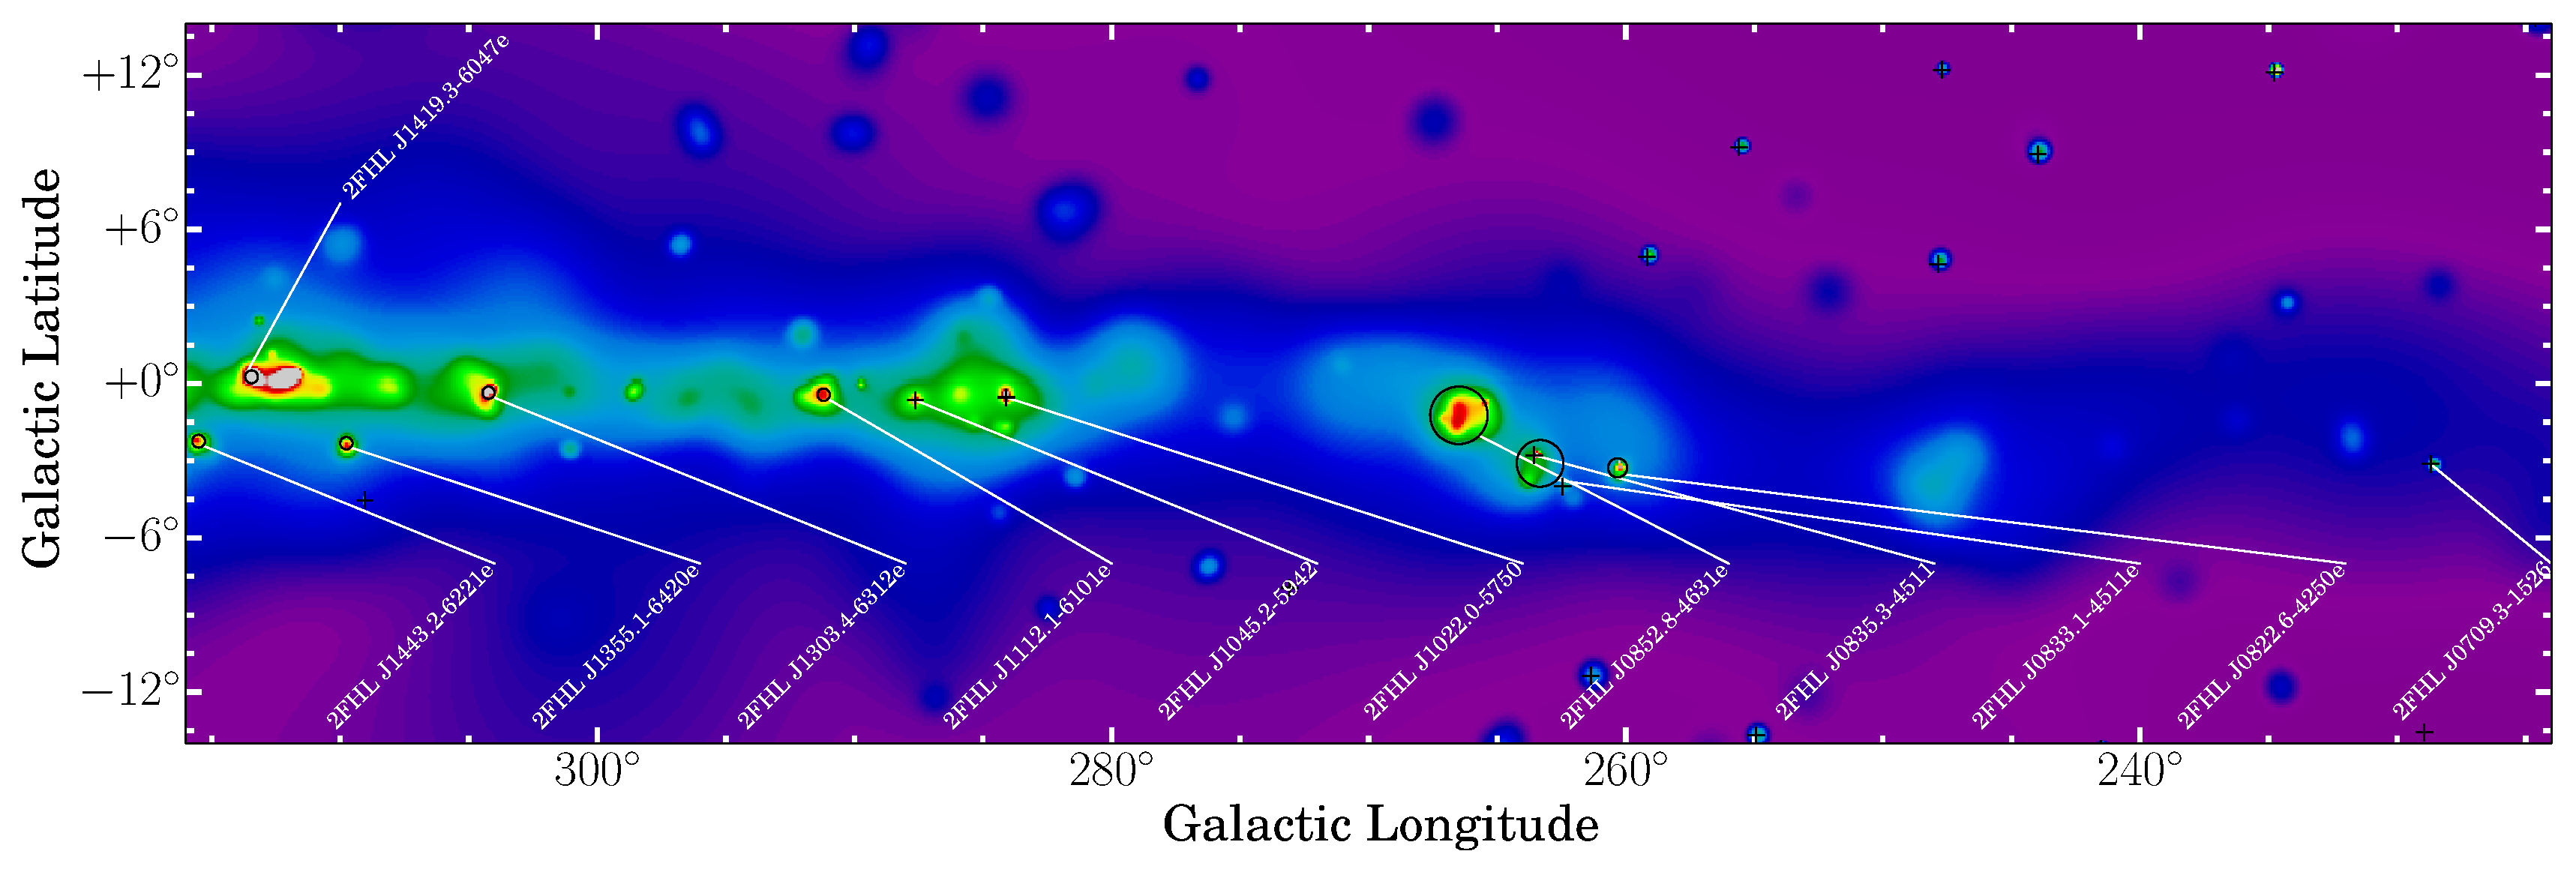
\includegraphics[angle=90,scale=.3]{Figures/Galactic_plane_CAR_4of4_sqrt_spectral_2FHL.eps}\\
            %\includegraphics[angle=90,scale=.3]{f5c.eps}&
            %\includegraphics[angle=90,scale=.3]{f5d.eps}\\
            
        \end{tabular}
    \end{center}
    \begin{flushleft}
        {Fig.~\ref{fig:gp1}.}---  continued
    \end{flushleft}
\end{figure*}

Galactic sources display on average hard spectra, which is a sign
of efficient particle acceleration. Roughly 55\% of all Galactic
sources have a spectral index lower than 2.2. For comparison, only 14\% of the { 2FHL} blazars
display such hard spectra. %With the exception of Eta Carinae (2FHL J1045.2-5942), all hard Galactic sources belong to either the PWN class (12 sources) or the SNR class (8 sources).
A sizable fraction (approximately 25\%, 
see Figure~\ref{fig:hist_index}, upper panel)
of Galactic sources has a photon
index harder than 2, implying a high-energy SED peak in the TeV band.
Indeed, as the lower panel of Figure~\ref{fig:hist_index} shows,
\lat{} detects emission from many Galactic sources well beyond 500\,GeV.
%All these sources belong to either the PWN or SNR classes.
All PWNe detected by {\it Fermi} are found to be powered by young
and energetic pulsars \citep[age $\lesssim 30$\,kyr,][]{Acero13}.
While it is common for PWNe to show hard spectra, this is less
so for SNRs whose majority (about 85\,\%) display softer spectra
\citep{snrCat}. Hard-spectrum SNRs are typically young or 
mid-aged ($\lesssim$3--5\,kyr)
and might be difficult to find in radio surveys. Thus, Galactic surveys
at above 50\,GeV have the capability to detect new SNRs that
might have been previously missed.
Such an example is represented by the extended source 
2FHL J0431.2+5553e which is spatially coincident with a 
new SNR (SNR G150.3+4.5) recently reported by \cite{Gao14} (see Chapter \ref{chap:G150}).

Of the 14 sources at $|b|<10^{\circ}$ that do not have an
association, 7 have power-law indices harder than 2
which renders them  likely Galactic objects.
It is interesting to note that { 6 of these 7 objects} are offset from the plane of the Galaxy  by more than $4^{\circ}$. This is in marked contrast with the 
associated portion of the sample where only the Crab Nebula and the
newly discovered SNR G150.3+4.5 (out of 34 SNR/PWN systems) have such
a large offset. Thus it seems unlikely that all these unassociated sources
are SNR/PWN systems.

%%%%%%%%%%%%%%%%%%%%%%%%%%%%%%%%%%%%%%%%%%%%%%%%%%%%%%%%%%
%
% H E S S 
%
%%%%%%%%%%%%%%%%%%%%%%%%%%%%%%%%%%%%%%%%%%%%%%%%%%%%%%%%%%%

\subsection{Comparison with the H.E.S.S. Galactic Plane Survey}\label{2fhl:HESS}
The H.E.S.S array, with a field of view of about 5$^{\circ}$ and an angular resolution of approximately 0.12$^\circ$, has invested 2800\,hrs of exposure to survey  part\footnote{The H.E.S.S. Galactic plane survey extends between 283$^{\circ}<l<$59$^{\circ}$ and Galactic latitudes of $|b|<3.5^{\circ}$.} 
of the Galactic plane, reaching an average sensitivity of 2\,\% of the Crab Nebula flux (i.e. 4.5$\times10^{-13}$\,ph~cm$^{-2}$~s$^{-1}$) at $\geq$1\,TeV \citep{aharonian06_gps,carrigan2013}. Considering that the Crab Nebula spectrum is harder
in the 2FHL band than in the $>$1\,TeV band, we estimate that the average sensitivity of 2FHL in the same region of the H.E.S.S. survey is $\sim$3--4\,\% of the { 50\,GeV--2\,TeV Crab Nebula flux.} The slightly better sensitivity 
allows H.E.S.S. to detect 69 sources (as reported in the TeVCat), while
the LAT finds 36 objects in the same area. However, the comparable sensitivities of the two surveys allow the study of the  properties of the high-energy Galactic population.
%%%% USE following to convert the 2% >1TeV Crab nebula flux to
%%%%     2FHL flux
%%%%  4.5e-13*(pow(2.,-1.3)-pow(50./1000.,-1.3))/(pow(100.,-1.3)-pow(1.,-1.3))
%%%%
%%%%  The HESS Crab has an index of 2.3
%%%%  The Fermi Crab has index of 2.13 and flux 1.31e-9 ph/cm2/s
In the 2FHL catalog there is almost an equal number of SNRs and PWNe
in contrast to what is found in the  H.E.S.S. survey where the ratio
of PWNe to SNRs is 1.5 to 1. This might be because
the hardest PWNe and softest SNRs { are difficult to detect} respectively
in the $>$50\,GeV and $>$1\,TeV bands.


Of the 36 2FHL sources that fall within the footprint of 
the H.E.S.S. survey, 23 have already been detected
at TeV energies and are associated with known counterparts,
while 7 are undetected. The remaining 6 objects
(2FHL~J1022.0$-$5750, 2FHL~J1505.1$-$5808,  2FHL~J1507.4$-$6213, 2FHL~J1703.4$-$4145, 2FHL~J1745.1$-$3035 and  2FHL~J1856.8+0256)
are spatially coincident with TeV sources whose origin is not known.
All of them have hard spectral indices ($\Gamma<$2.2), but
it is interesting to note that 4 of them 
(2FHL~J1022.0$-$5750, 2FHL~J1505.1$-$5808, 2FHL~J1703.4$-$4145, and 2FHL~J1745.1$-$3035)
have $\Gamma<1.7$ (see also Figure~\ref{fig:gal_sed}).

We find that 2FHL~J1022.0$-$5750 is spatially compatible with
{ HESS~J1023$-$575, an extended TeV source \citep{westerlund2_hess11},
    whose emission might be due to a PWN powered by PSR~J1023$-$5746 \citep{Acero13}. }
%Westerlund 2 (TeV~J1023$-$5747), a massive star cluster already detected as an extended source at TeV energies \citep{westerlund2_hess11}.
2FHL~J1505.1$-$5808 is spatially coincident with the unidentified
object HESS~J1503$-$582, which has a size of 0.26$^{\circ}$ and a flux above 1\,TeV \citep{renaud08} compatible with the extrapolation of the 2FHL J1505.1$-$5808 spectrum.
Its spectrum, reminiscent of that of a PWN 
\citep[\eg{}, HESS~J1825$-$137,][]{grondin2011},
 is reported in Figure~\ref{fig:gal_sed}.


2FHL~J1507.4$-$6213 is spatially coincident with HESS~J1507$-$622, an extended source with a radius of 0.15$^{\circ}$ located  3.5$^{\circ}$ from the plane \citep{acero11}. The analysis of multiwavelength data showed that it is not possible to discriminate between a hadronic and leptonic origin of the emission, but that the latter scenario, if the emission is powered by a PWN, would require a pulsar generated in the explosion of a hyper-velocity star in order to reach the required distance from the plane \citep{domainko2012}.



The sources 2FHL~J1703.4$-$4145 and 2FHL~J1745.1$-$3035 are the hardest sources ($\Gamma<1.3$) among the six objects.
2FHL~J1703.4$-$4145 is spatially coincident with the bright radio emission
observed from the western side of the shell of SNR G344.7$-$001,
a nearby mid-aged  shell-type (age $\sim3000$\,yr and 8$'$ diameter) SNR \citep{giacani2011}. Both the 2FHL source and the SNR are spatially coincident
with the larger, elongated and unidentified HESS~J1702$-$420 \citep{aharonian08}.
It thus seems likely that  SNR G344.7$-$001 is the  counterpart
of  2FHL J1703.4$-$4145 and perhaps also of HESS~J1702$-$420.
The combined {\it Fermi}-H.E.S.S. spectrum of this source is reported in Figure~\ref{fig:gal_sed}.



2FHL~J1745.1$-$3035 is found to be spatially coincident with 
the extended source HESS~J1745$-$303, which may be comprised of
up to three different sources \citep{aharonian2008_j1745}. Indeed, the position of
2FHL~J1745.1$-$3035 is compatible  with the 'C' emission
region \citep[the second brightest region in the complex,][]{aharonian2008_j1745}.
However, the nature of this source is more complex, because
the 2FHL source is marginally brighter at 1\,TeV than the entire H.E.S.S. region and also has a harder spectrum (spectral index of 1.25$\pm0.38$ in 2FHL 
versus $2.17\pm 0.11$ as measured by H.E.S.S.).

Finally, 2FHL~J1856.8+0256 is coincident with HESS~J1857+026, an almost radially symmetric extended source  \citep{aharonian08_unid}, whose emission likely originates from a PWN powered by PSR~J1856+0245 \citep{rosseau2012}.

\begin{figure*}[ht]
    \begin{center}
       \hspace*{-1.5cm} \begin{tabular}{ll}
            \includegraphics[width=8cm]{Figures/{J0617.2+2234e_SED}.eps} &
            \includegraphics[width=8cm]{Figures/{J1419.3-6047e_SED}.eps}\\
            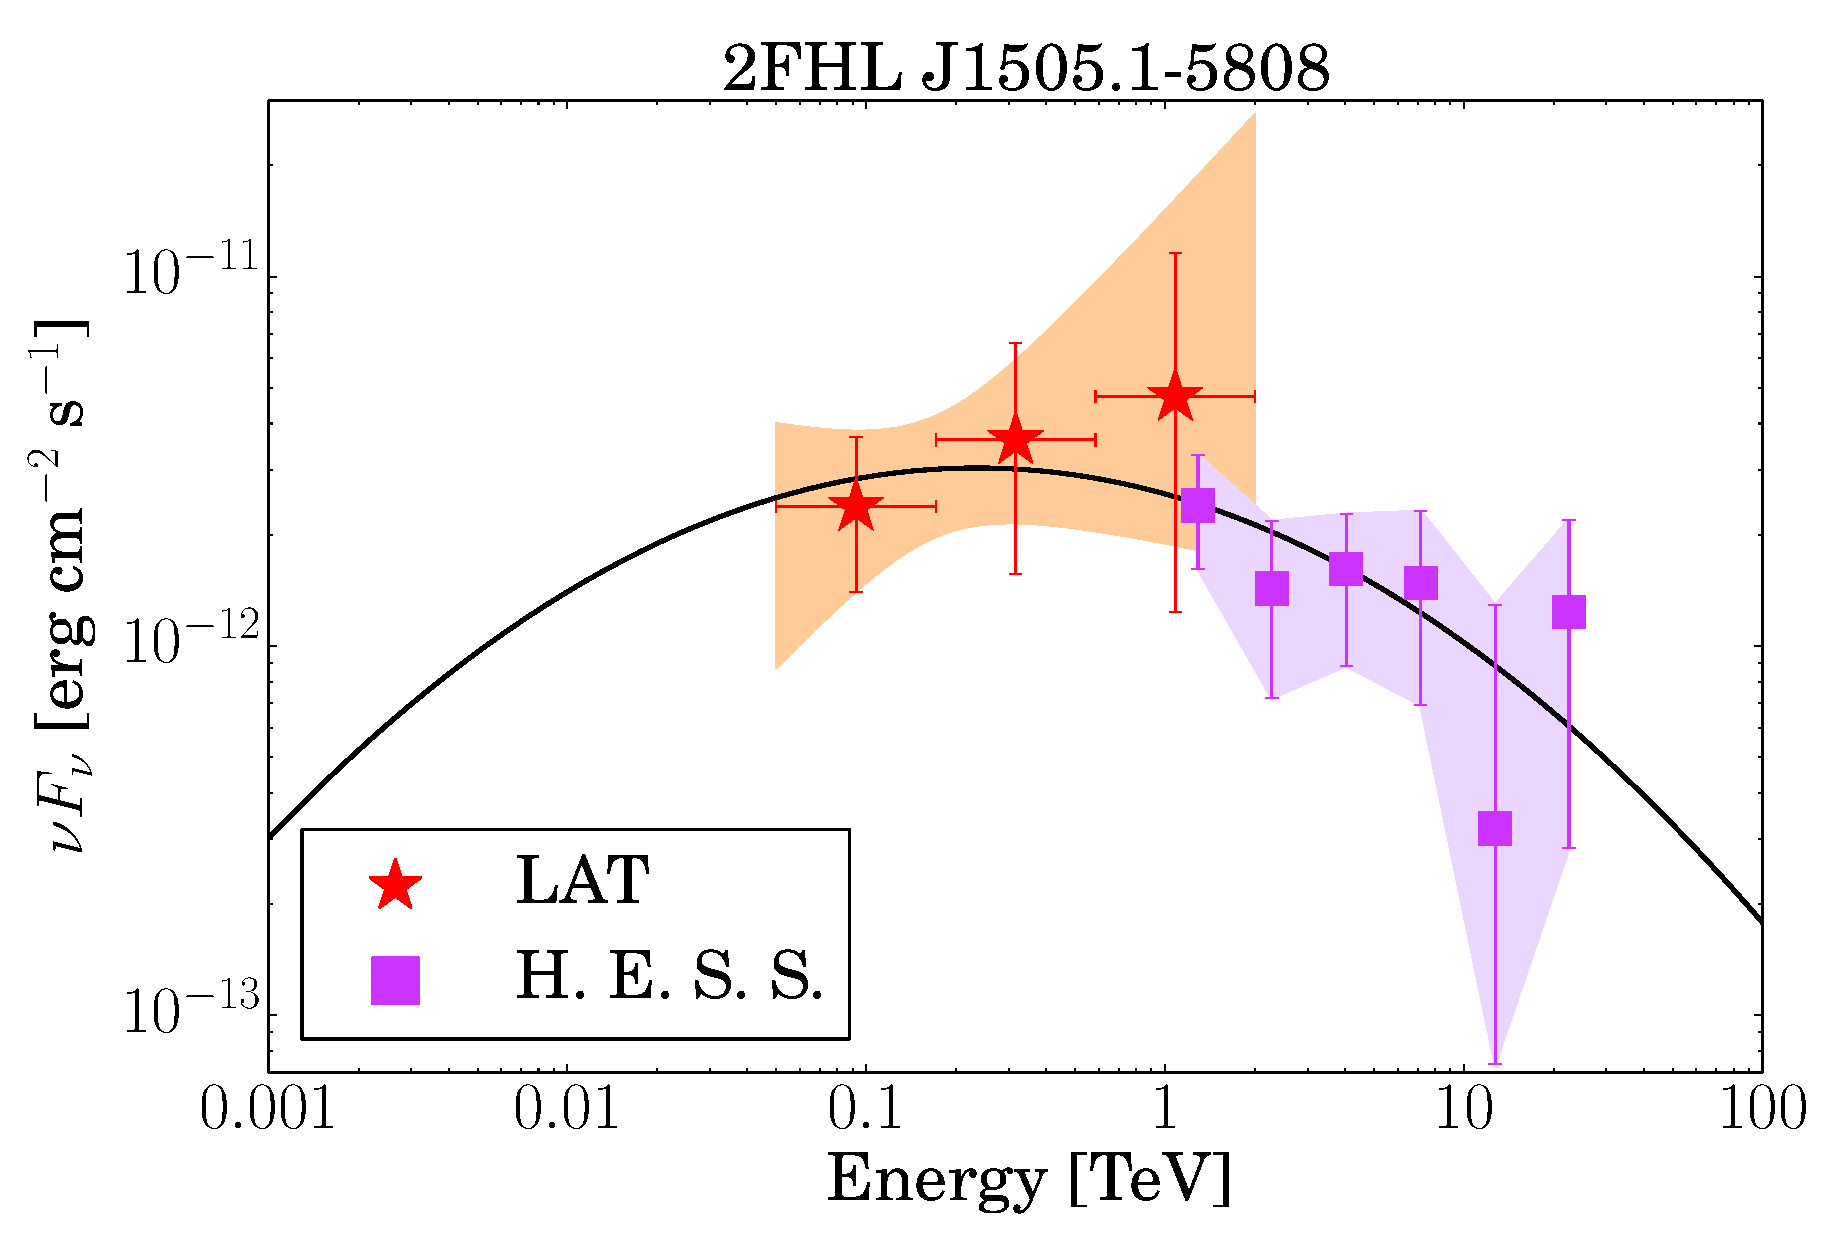
\includegraphics[width=8cm]{Figures/pgw_00682_SED.eps} &
            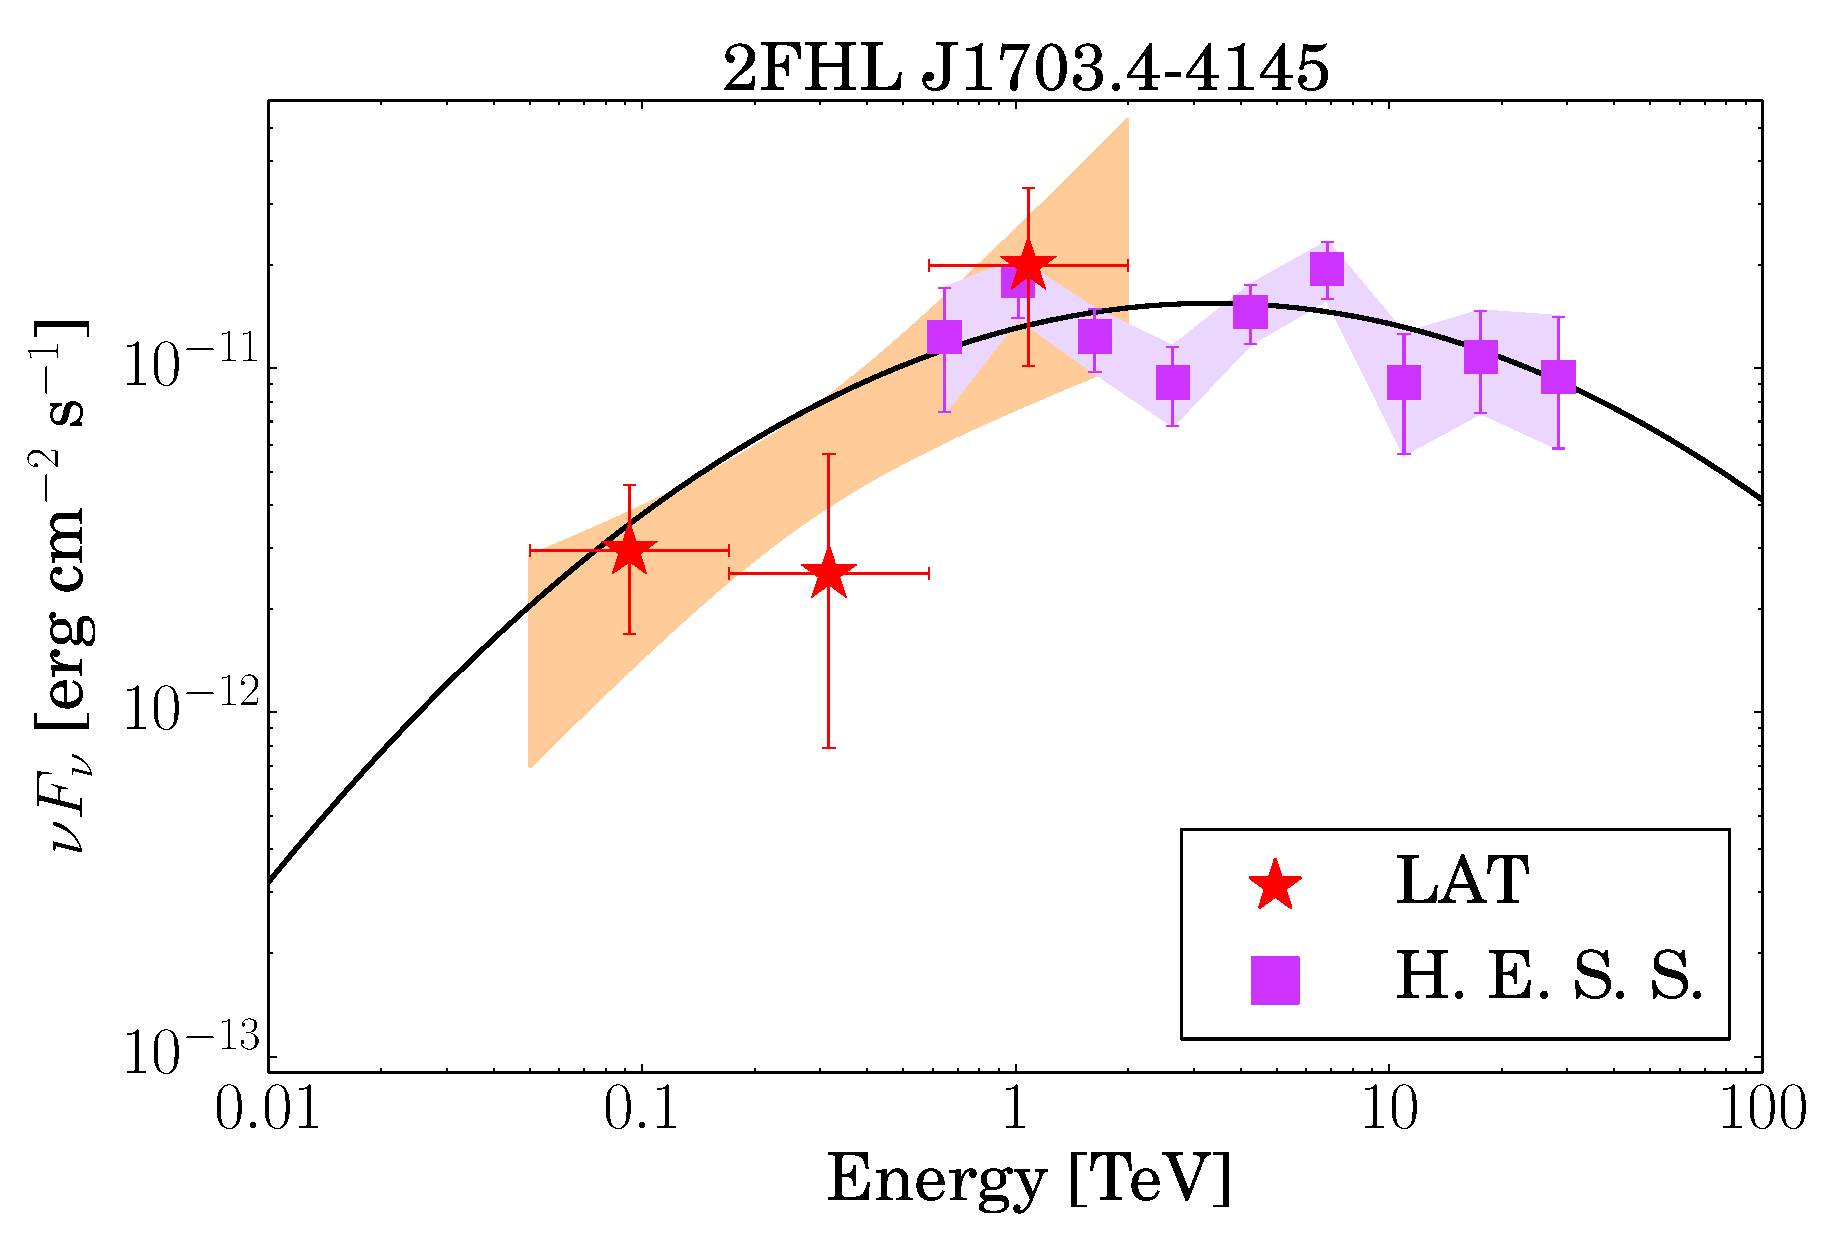
\includegraphics[width=8cm]{Figures/pgw_00110_SED.eps} \\
        \end{tabular}
    \end{center}
    \caption{
        \label{fig:gal_sed}Spectral energy distributions of four Galactic sources constructed by combining data from the 3FGL (green diamonds), 1FHL (blue circles), and 2FHL (red stars). We show the 3FGL extended source SNR IC~443 (\emph{top left}), the new 2FHL extended source PSR~J1420$-$6048 (\emph{top right}), and two ``dark accelerators'' detected by H.E.S.S. at TeV energies \citep[][purple squares]{carrigan2013} without a previous LAT counterpart:  { HESS~J1503$-$582} (\emph{bottom left}) and HESS~J1702$-$420 (\emph{bottom right}).}
\end{figure*}

%%%%%%%%%%%%%%%%%%%%%%%%%%%%%%%%%%%%%%%%%%%%%%%%%%%%%%%%%%%%%%%%%%%
%
%  Extended Source Results
%
%%%%%%%%%%%%%%%%%%%%%%%%%%%%%%%%%%%%%%%%%%%%%%%%%%%%%%%%%%%%%%%

\subsection{\label{2fhl:ESresults}Extended Source Results}


In total, 31 sources are modeled as spatially extended and input into the ML analysis: 25 listed in 3FGL, 5 sources detected in the {\tt pointlike} analysis (described in Chapter \ref{2fhl:3FGL_ES}) that were not { detected as extended at the time of} 3FGL, and one, SNR W41, reported  recently by both the H.E.S.S. and LAT teams \citep{HESSLATW41}. Names and properties of the extended sources  are provided in Tables \ref{tab:extended} and \ref{tab:new_extended}. 
Six extended sources, detected in 3FGL, were not detected in 2FHL: the SMC, S~147 ({the point source 2FHL~J0534.1+2753 was detected inside it}), the lobes of Centaurus A (although we detect its core as a point source, 2FHL J1325.6$-$4301), W~44, HB~21 and the Cygnus Loop.

We detect a weak source, 2FHL~J1714.1$-$4012 (TS = 27), just outside the southwestern edge of the 3FGL spatial template used to model the emission from SNR RX J1713.7$-$3946 (2FHL~J1713.5$-$3945e). 2FHL~J1714.1$-$4012 has a hard spectral index $\Gamma = 1.63 \pm 0.38$, that is within errors of the spectral index derived for the SNR, $\Gamma = 2.03 \pm 0.20$ \citep{Abdo11-RXJ1713}. It is unclear whether 2FHL~J1714.1$-$4012 is a distinct source separated from the SNR, or the result of un-modeled residual emission due to an imperfection in the spatial template adopted for the extended source.


2FHL~J1836.5$-$0655e is associated with the PWN HESS J1837$-$069. The 3FGL catalog contains  several point sources in the vicinity of the PWN. We detect three sources in the vicinity, 2FHL~J1834.5$-$0701, 2FHL~J1837.4$-$0717 and 2FHL~J1839.5 ~ $-$0705, the first two of which are coincident with 3FGL sources (3FGL J1834.6$-$0659, 3FGL J1837.6$-$0717 respectively). The power-law spectral indices of the three 2FHL point sources and 2FHL J1836.5$-$0655e are all consistent with each other. The concentration of sources around HESS J1837$-$069 combined with the spectral compatibility of the sources is suggestive of a common origin to the $\gamma$-ray emission in this region. However, the surrounding $\gamma$ rays could arise from other sources in the region \citep{Gotthelf08}; further analysis is necessary to determine the nature of the sources in this region. 

A brief description of the five new 2FHL extended sources is given below with residual TS maps for the region surrounding each source shown in Figure \ref{fig:6ES}. Detailed analyses of these new extended sources will be reported in separate papers.


{\bfseries 2FHL~J1443.2$-$6221e} overlaps with the young, radio-detected SNR RCW 86 (G315.4−2.3). RCW 86 is a 42$'$ diameter SNR that lies at a distance of 2.3-2.8 kpc and is likely associated with the first recorded supernova, SN 185 AD \citep{Rosado96,Sollerman03}. With more than 40 months of data and using the  P7SOURCE dataset, the LAT did not significantly detect the SNR, but upper limits on detection at GeV energies combined with detection of significant extension in the TeV \citep{Aharonian09} were sufficient to strongly favor a leptonic origin for the emission \citep{Lemoine-Goumard12}.

An updated LAT analysis of RCW~86 using 76 months of data, as well as the Pass 8 event-level analysis, resulted in detection of the SNR by the LAT as well as significant extension measurement \citep[the former published after \cite{2FHL}]{Ajello_rcw86,Hewitt15a}. In this paper, we report the results derived for 2FHL~J1443.2$-$6221e from the {\tt pointlike} analysis described in Chapter \ref{2fhl:3FGL_ES}.

{\bfseries 2FHL~J1419.2$-$6048e} is a newly detected extended sources with size
 ${\rm \sigma_{disk} =}$ ${\rm 0.36 ^{\circ} \pm}$ $0.03 ^{\circ}$, that overlaps two nearby PWN/PSR complexes in the Kookaburra region. In the southwest of Kookaburra, HESS~J1418$-$609 \citep{AharonianKook06} is coincident with both the extended non-thermal X-ray ``Rabbit" PWN \citep[G313.3+0.1,][]{Roberts99}, and the $\gamma$-ray detected pulsar PSR~J1418$-$6058 \citep{AbdoBlindPSR09}. The northeast region, called ``K3", contains HESS~J1420$-$607, coincident with PWN~G313.5+0.3 and PSR J1420$-$6048. \cite{Acero13} detected, with \lat, emission from both HESS~J1418$-$609 (with a soft spectral index, pulsar-like spectrum) and HESS~J1420$-$607 (with a hard power-law index) above 10 GeV, but only HESS J1420$-$607 was significantly detected above 30 GeV. Neither showed significant extension. Our result for the fitted power-law spectral index of 2FHL~J1419.2$-$6048e is in agreement with the previous GeV and TeV results, yet our measured radius is considerably larger than the TeV extension. To compare the extensions of the uniform disk model used for 2FHL~J1419.2$-$6048e in this paper to the Gaussian model of \cite{AharonianKook06}, we defined the radius which contains 68\% of the source's intensity as r$_{68}$, with ${\rm r_{68,Gaussian} = 1.51\sigma}$, and ${\rm r_{68,disk} = 0.82\sigma}$  \citep{Lande12}. We find that ${\rm r_{68} \simeq 0.30^{\circ}}$ for 2FHL~J1419.2$-$6048e, and ${\rm r_{68}} \simeq 0.09^{\circ}$ for HESS~J1420$-$607. \jamie{Include details on the small kookaburra study if I have time}

{\bfseries 2FHL J1355.2$-$6430e}, coincident with the VHE source HESS J1356$-$645, is detected as extended (${\rm \sigma_{disk} =  0.57^{\circ} \pm 0.02^{\circ}}$) for the first time by the LAT in this work. The  source HESS J1356$-$645 \citep{Abramowski11} is associated with the pulsar PSR J1357$-$6429, which was determined to be powering a surrounding extended radio and X-ray PWN \citep{Lemoine-Goumard11}. \cite{Acero13} detected faint emission from the nebula, and derived a 99\% confidence limit, Bayesian upper limit on extension (${\rm \sigma_{Gauss} < 0.39^{\circ}}$) in the absence of significant extension. The fitted spectral index for 2FHL J1355.2$-$6430e is compatible with the GeV and TeV results \citep{Acero13,Abramowski11}, however, the fitted disk extension is larger than that of the TeV detection, with ${\rm r_{68} \simeq 0.47^{\circ}}$ for 2FHL~J1355.2$-$6430e and ${\rm r_{68}}$ $\simeq 0.30^{\circ}$ for HESS~J1356$-$645.

{\bfseries 2FHL J1112.4$-$6059e} is an extended source (${\rm \sigma_{disk} =  0.53^{\circ} \pm 0.03^{\circ}}$) newly detected by the LAT that encircles two 3FGL sources, 3FGL J1111.9$-$6058 and 3FGL J1111.9$-$6038, and has another, 3FGL J1112.0$-$6135, just outside its boundary \citep{3FGL}. The extended source also partially overlaps the massive star forming region NGC 3603. %A detailed LAT analysis of this region is underway and will be presented elsewhere. % MA COMMENTED it. in \jamie{need a ref for Junichiro's work}.

Finally, {\bfseries 2FHL J0431.2+5553e} is a large extended source (${\rm \sigma_{disk} =  1.27^{\circ} \pm 0.04^{\circ}}$), with { a hard spectrum}, that has not been previously detected at $\gamma$-ray energies. It overlaps the recently discovered radio SNR G150.3+4.5 \citep{Gao14}. G150.3+4.5 is a ${\rm 2.5^{\circ}}\times {\rm 3^{\circ}}$ (Galactic coordinates)
% wide (GLON) and ${\rm 3^{\circ}}$ high (GLAT) 
elliptical shell type SNR that has a steep radio synchrotron spectrum ($\alpha = -0.6$), indicative of radio SNRs. An in depth LAT analysis of this source extending the energy down to $E > 1$~GeV is presented in Chapter \ref{chap:G150}

\begin{figure*}[ht]
    \begin{center}
         \hspace*{-1.5cm}\begin{tabular}{ll}
            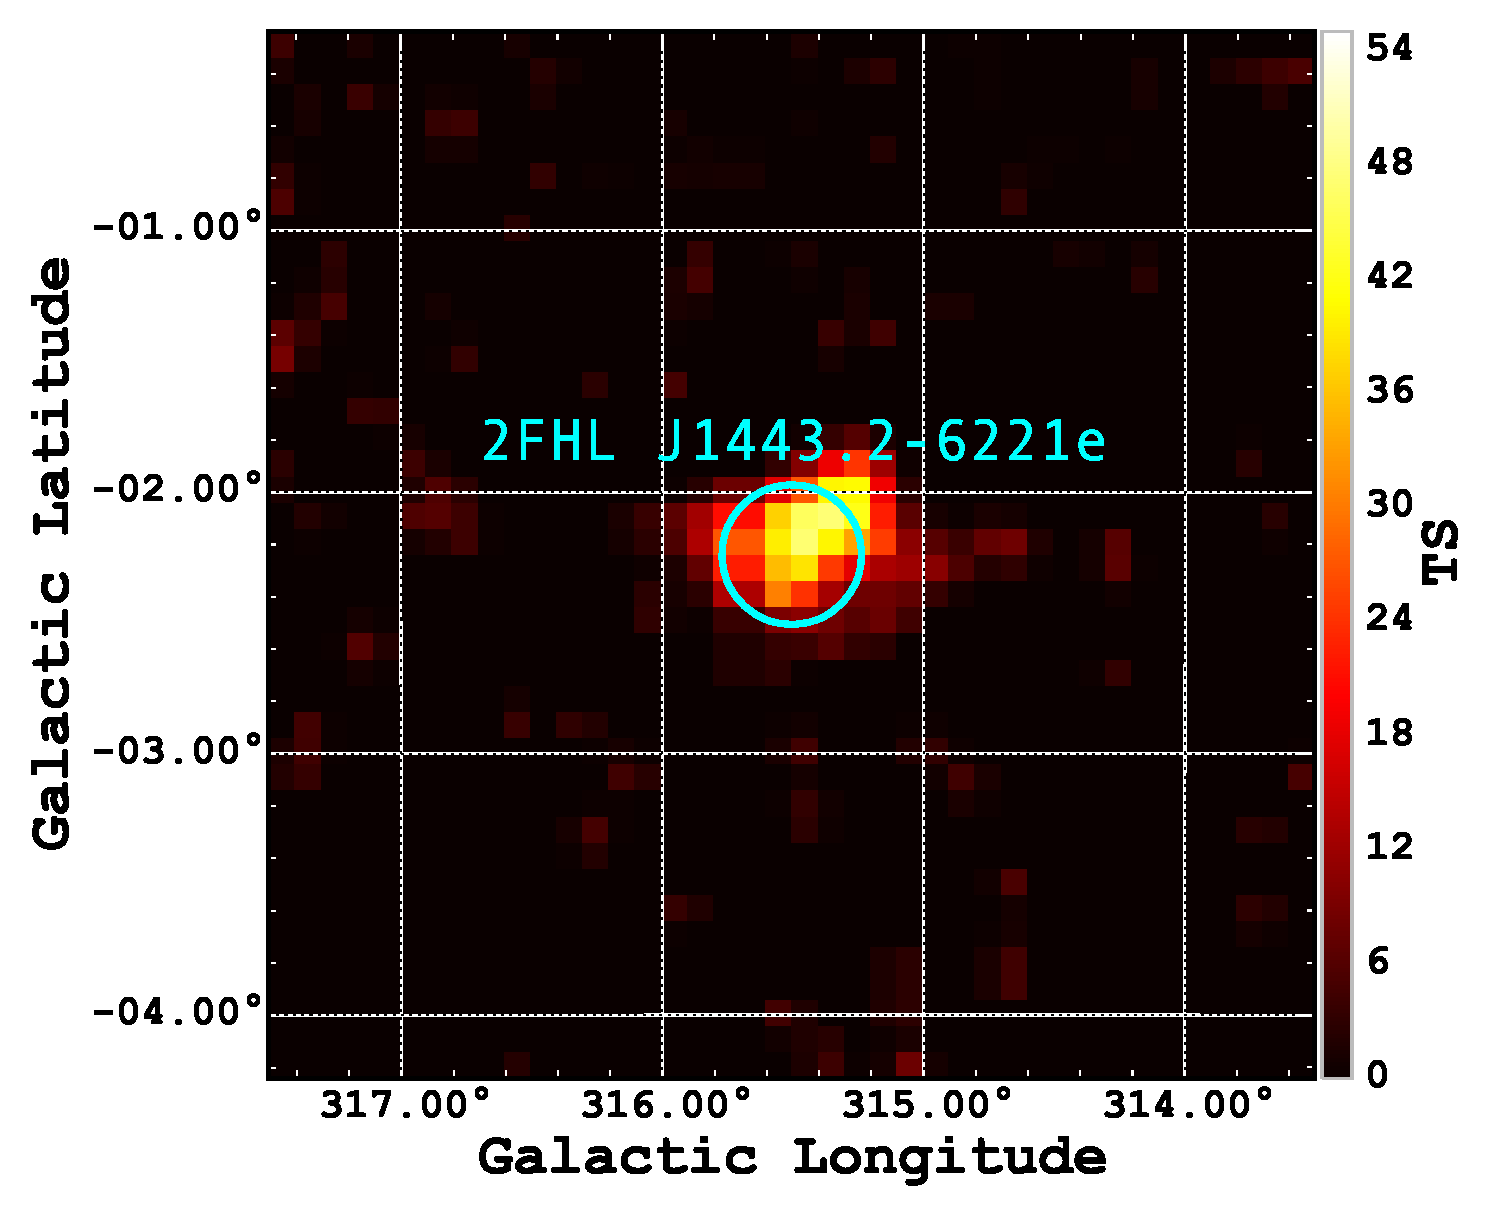
\includegraphics[width=8cm]{Figures/l315_b0_ES_3_residTSmap_2FHL_zoom.eps} &
            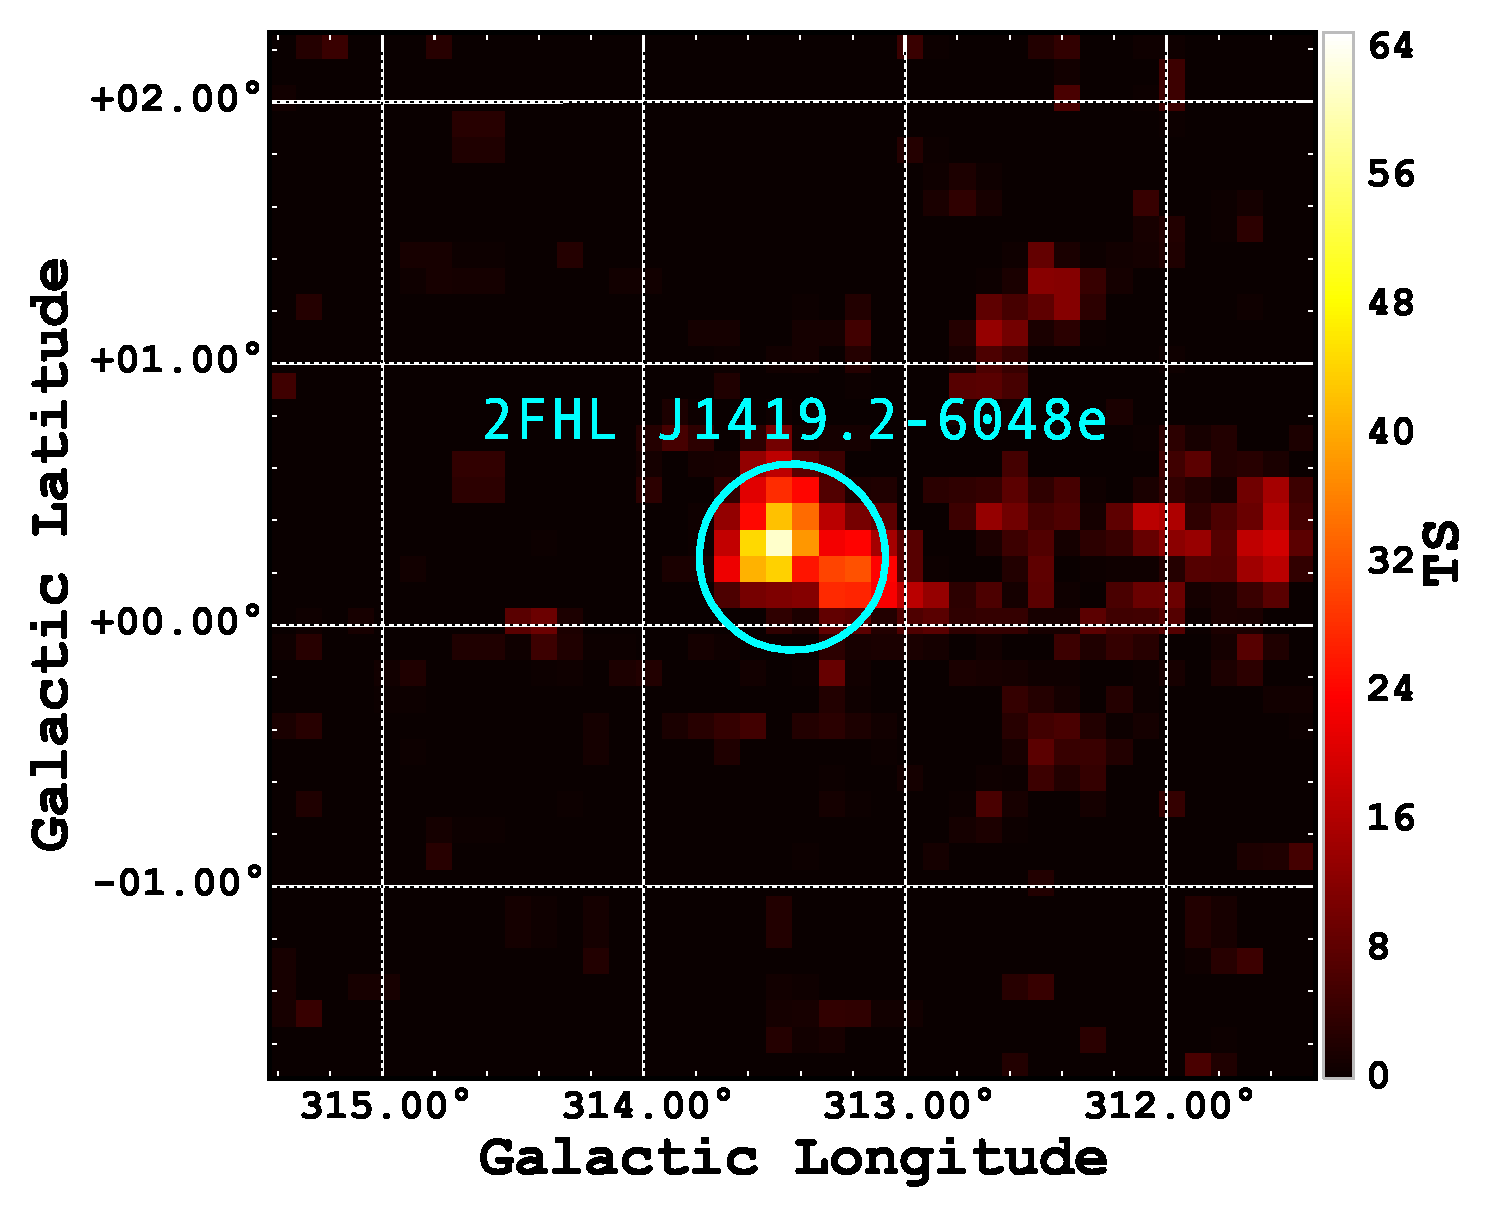
\includegraphics[width=8cm]{Figures/l315_b0_ES_4_residTSmap_2FHL_zoom.eps}\\
            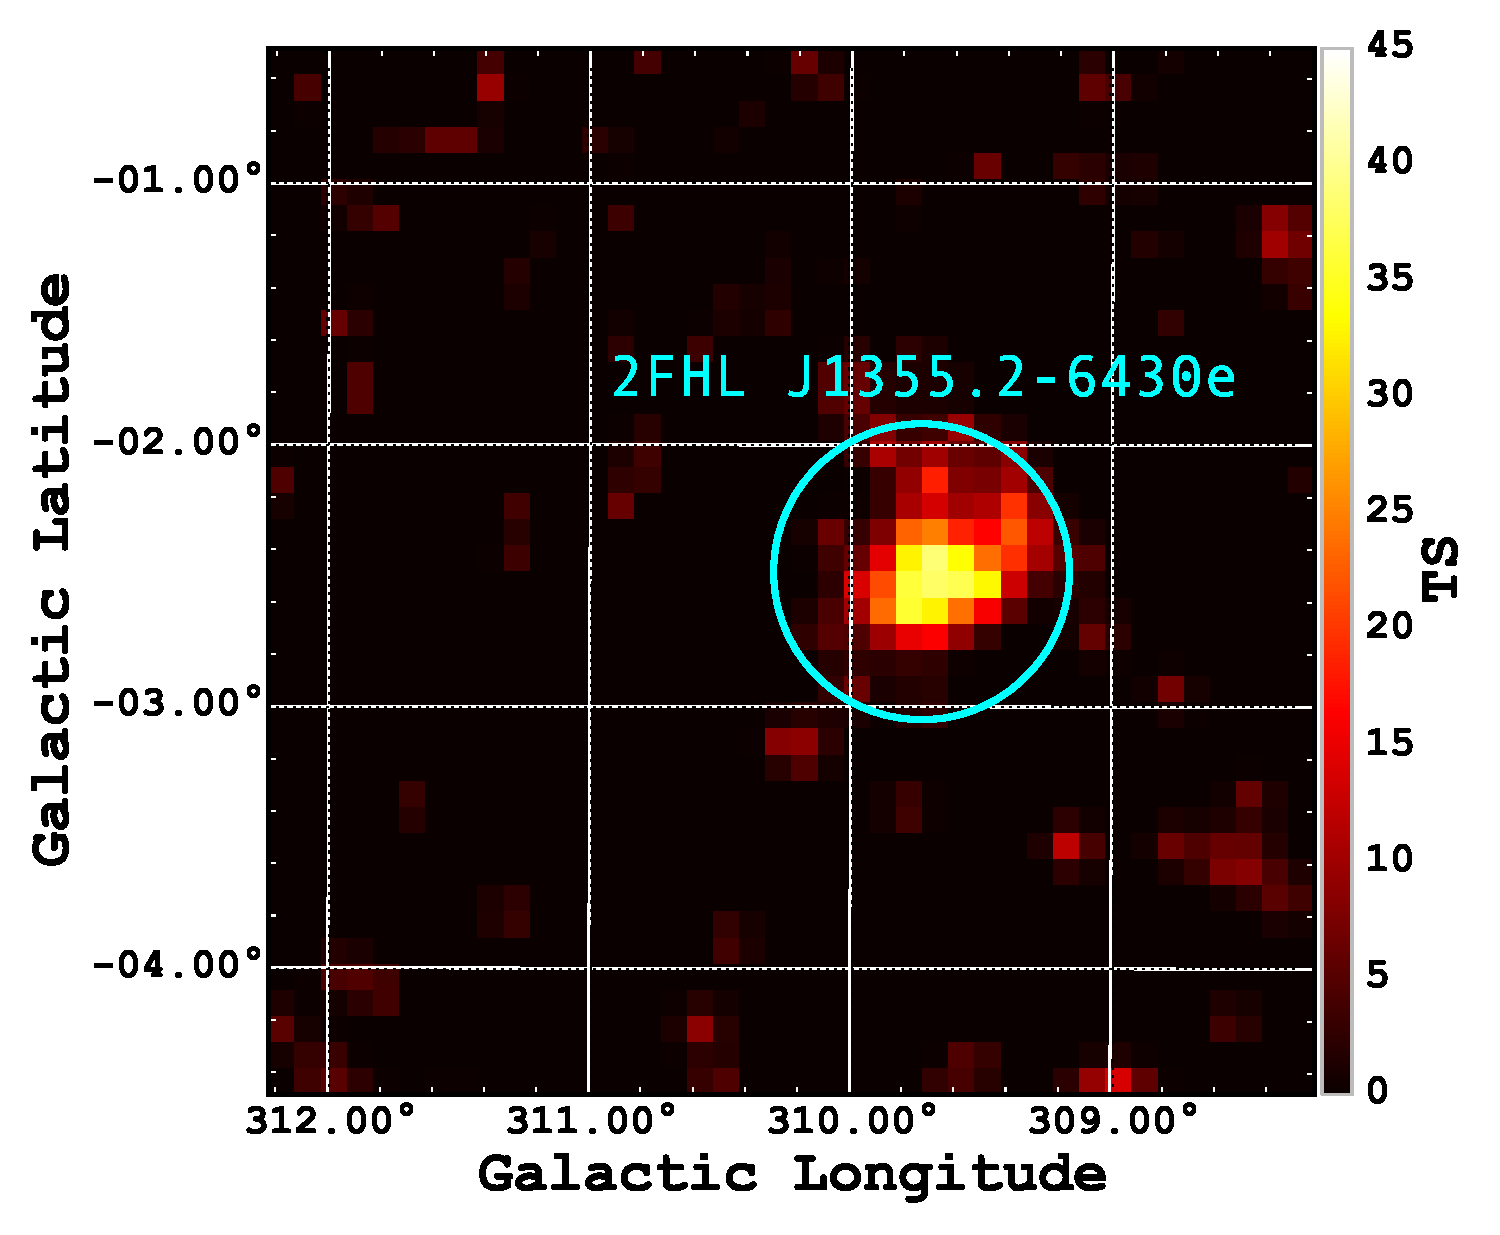
\includegraphics[width=8cm]{Figures/l315_b0_ES_1_residTSmap_2FHL_zoom.eps} &
            \includegraphics[width=8cm]{Figures/l290_b0_ES_1_residTSmap_2FHL_zoom.eps} \\
            \multicolumn{2}{c}{\includegraphics[width=8cm]{Figures/l145_b0_ES_1_residTSmap_2FHL_zoom.eps} }\\
        \end{tabular}
    \end{center}
    \caption{
        \label{fig:6ES} Residual TS maps for the five new extended sources described in Chapter \ref{2fhl:ESresults}.  Only the Galactic diffuse and isotropic emission are included in the model to highlight the location of emission not associated with the diffuse background. Circles indicate the extents of the fit disks. {The x marker in the bottom panel (2FHL~J0431.2+5553e) shows the location of a point source in the \roi{}.}}
\end{figure*}

\begin{deluxetable}{lccclccc}
\setlength{\tabcolsep}{0.04in}
\tablewidth{0pt}
\tabletypesize{\scriptsize}
\tcap{2FHL extended sources previously detected by the {\it Fermi}-LAT \label{tab:extended}}
\tablehead{
\colhead{2FHL Name} & 
\colhead{$l$ [deg]} & 
\colhead{$b$ [deg]} &
\colhead{TS} &
\colhead{Association} &
\colhead{Class} &
\colhead{Spatial model} &
\colhead{Radius [deg]}
}
\startdata
 J0526.6$-$6825e      &    278.843 &    -32.850 & 49.80  & LMC                & gal    & 2D Gaussian 		& 1.87 \\
 J0617.2+2234e        &    189.048 &      3.033 & 398.64 & IC~443             & snr    & 2D Gaussian 		& 0.27 \\
 J0822.6$-$4250e      &    260.317 &	 -3.277 &  63.87 & Puppis A	      & snr    & Disk	     		& 0.37 \\
 J0833.1$-$4511e      &    263.333 &     -3.104 & 49.70  & Vela~X             & pwn    & Disk        		& 0.91 \\
 J0852.8$-$4631e      &    266.491 &     -1.233 & 437.21 & Vela~Jr            & snr    & Disk        		& 1.12 \\
 J1303.4$-$6312e      &    304.235 &     -0.358 & 56.06  & HESS~J1303$-$631   & pwn    & 2D Gaussian 		& 0.24 \\
 J1514.0$-$5915e      &    320.269 &     -1.276 & 165.51 & MSH~15$-$52        & pwn    & Disk        		& 0.25 \\
 J1615.3$-$5146e      &    331.659 &     -0.659 & 128.15 & HESS~J1614$-$518   & spp    & Disk        		& 0.42 \\
 J1616.2$-$5054e      &    332.365 &     -0.131 & 87.18  & HESS~J1616$-$508   & pwn    & Disk        		& 0.32 \\
 J1633.5$-$4746e      &    336.517 &      0.121 & 114.17 & HESS~J1632$-$478   & pwn    & Disk        		& 0.35 \\
 J1713.5$-$3945e      &    347.336 &     -0.473 & 60.98  & RX~J1713.7$-$3946  & snr    & Map         		& 0.56 \\
 J1801.3$-$2326e      &      6.527 &     -0.251 & 50.20  & W~28               & snr    & Disk        		& 0.39 \\
 J1805.6$-$2136e      &      8.606 &     -0.211 & 160.43 & W~30               & snr    & Disk        		& 0.37 \\
 J1824.5$-$1350e      &     17.569 &     -0.452 & 266.09 & HESS~J1825$-$137   & pwn    & 2D Gaussian 		& 0.75 \\
 J1834.9$-$0848e      &     23.216 &     -0.373 &  67.30 & W~41               & spp    & 2D Gaussian		& 0.23 \\
 J1836.5$-$0655e      &     25.081 &      0.136 & 62.72  & HESS~J1837$-$069   & pwn    & Disk        		& 0.33 \\
 J1840.9$-$0532e      &     26.796 &     -0.198 & 163.15 & HESS~J1841$-$055   & pwn    & Elliptical 2D Gaussian & 0.62, 0.38, 39 \\
 J1923.2+1408e        &     49.112 &     -0.466 & 44.60  & W~51C              & snr    & Elliptical Disk        & 0.38, 0.26, 90 \\
 J2021.0+4031e        &     78.241 &      2.197 & 115.97 & Gamma Cygni        & snr    & Disk                   & 0.63 \\
 J2028.6+4110e        &     79.601 &      1.396 & 28.09  & Cygnus Cocoon      & sfr    & 2D Gaussian            & 3.0 \\
\enddata
\tablecomments{~List of the 20 extended sources in 2FHL that were previously detected as extended by the {\it Fermi}-LAT. All these sources are in  3FGL except W41, which is studied by \citet{W41}. The Galactic coordinates $l$ and $b$ are given in degrees. The extension of the disk templates is given by the radius. The extension of the 2D Gaussian templates is given by the $1\sigma$ radius, and the elliptical templates are given by the semi-major axis, semi-minor axis, and position angle (East of North). Association, Class, and Spatial model are as given in \threefgl{}.
}
\end{deluxetable}


\begin{deluxetable}{lcccccccclccc}
\setlength{\tabcolsep}{0.04in}
\tablewidth{0pt}
\tabletypesize{\scriptsize}
\tcap{New 2FHL extended sources 
\label{tab:new_extended}}
\tablehead{
\colhead{2FHL Name} & 
\colhead{$l$ [deg]} & 
\colhead{$b$ [deg]} &
\colhead{TS} & 
\colhead{TS$_{ext}$} &
\colhead{TS$_{2pts}$} &
\colhead{$F_{50}$} & 
\colhead{$\Delta F_{50}$} &
\colhead{$\Gamma$} & 
\colhead{$\Delta \Gamma$} &
\colhead{Association} &
\colhead{Class} &
\colhead{Radius [deg]} 
}
\startdata
 J0431.2+5553e        &    150.384 &      5.216 &  87.9 & 83.4  & 26.2    &  11.70 &       2.11 &    1.66 &         0.20 & G~150.3+4.5     & snr     & 1.27 $\pm$  0.04 \\
 J1112.4$-$6059e      &    291.222 &     -0.388 &  80.9 & 68.3   & 22.5    &  12.80 &       2.36 &    2.15 &         0.28 & PSR~J1112$-$6103  & pwn     & 0.53 $\pm$ 0.03 \\
 J1355.2$-$6430e      &    309.730 &     -2.484 &  82.3 & 31.8   & 12.9     &  9.59  &       1.95 &    1.56 &         0.22 & PSR~J1357$-$6429  & pwn     & 0.57 $\pm$ 0.02 \\
 %J1407.3$-$6116e      &    311.924 &      0.259 &  68.66 & 30.00       &  14.70 &       2.63 &    2.58 &         0.28 & \nodata         & \nodata & 0.38 \\
 J1419.2$-$6048e      &    313.432 &      0.260 & 109.3 & 49.1   & 15.6    &  17.60 &       2.80 &    1.87 &         0.19 & PSR~J1420$-$6048  & pwn     & 0.36 $\pm$ 0.03  \\
 J1443.2$-$6221e      &    315.505 &     -2.239 &  75.6 & 29.9   & 19.2   &  7.23  &       1.70 &    2.07 &         0.30 & SNR~G315.4$-$2.3  & snr     & 0.27 $\pm$  0.03 \\
\enddata
\tablecomments{~List of the 5 new extended sources in 2FHL. All sources are characterized by a uniform disk template whose radius and uncertainty therein is given in the last column. $l$ and $b$ are Galactic coordinates. All coordinates are shown in degrees. TS is the test statistic. ${\rm TS_{ext}} $ is the signicance of extension (\ref{2fhl:newES}). TS$_{2pts}$ is the TS of two simultaneously fit point sources  (\ref{2fhl:newES}). $F_{50}$ and $\Delta F_{50}$ are the integrated photon flux between 50~GeV and 2~TeV and its uncertainty in units of $10^{-11}$~photon~cm$^{-2}$~s$^{-1}$. $\Gamma$ and $\Delta \Gamma$ are the photon  index and its uncertainty from a power-law fit. Association lists the primary overlapping source and Class the suspected source type.  All uncertainties are $1\sigma$ uncertainties.}
\end{deluxetable}



%%%%%%%%%%%%%%%%%%%%%%%%%%%%%%%%%%%%%%%%%%%%%%%%%%%%%%%%%%%%%%%%
%
%         Summary
%
%%%%%%%%%%%%%%%%%%%%%%%%%%%%%%%%%%%%%%%%%%%%%%%%%%%%%%%%%%%%%%%%
\section{Summary}
\label{sec:summary}

We have presented an all-sky analysis at $\geq$ 50\,GeV
of 80\,months of \lat{} data relying on the new Pass~8 event-level analysis.
Pass~8 delivers improvements in the acceptance and the PSF, reduces
background of misclassified charged particles
and extends the energy range at which the \lat{} is sensitive.
All this allowed the \lat{} to detect 360 sources in the 50\,GeV--2\,TeV range,
performing an unbiased census of the $>$50\,GeV sky for the first time.
%This is the first time that \lat can thoroughly explore this energy range.
This catalog of sources (dubbed 2FHL) provides a bridge between
the traditional 0.1--100\,GeV band of \lat{} catalogs \citep{3FGL}
and the $\gtrsim$100\,GeV band probed by IACTs from the ground.
The 2FHL catalog has the potential to improve the efficiency with
which new sources are detected at TeV energies since only
about 25\,\% of the 2FHL sources were previously detected by IACTs.

%The majority ($\gtrsim$80\,\%)of sources detected in the 2FHL catalog are likely extragalactic because they are either located at high Galactic latitude or are associated with blazars. 

2FHL includes 103 sources in the direction of the Galactic plane ($|b|<10^{\circ}$).
While a fraction of the sources ($\sim$39\,\%) are associated with blazars, the rest
are Galactic and unassociated sources. Galactic sources generally display
much harder photon indices than blazars (median of $\sim$2 versus $\sim$3)
and copious TeV emission, both signs of efficient particle acceleration.
Most Galactic sources are associated with PWNe and SNRs, systems at the end
of the stellar evolution cycle, and are detected as spatially extended.
All the hard (spectral index $<2$) unassociated  sources within the plane
of our Galaxy are likely of Galactic origin, since very few blazars 
have spectra as hard.

The Pass~8 event-level analysis  and accumulated exposure allow the LAT to extend its reach
to higher energy and to open a new window on the sub-TeV sky. Sensitivity improves linearly with time in the photon-limited regime, thus 
further observations by the LAT in the coming years
will probe the $>$\,50\,GeV sky even more deeply, providing
important targets for current and future 
Cherenkov telescopes.

%%%%%%

\chapter{Fermi-LAT Observations of Extended Gamma-Ray Emission in the Direction of SNR G150.3+4.5.}
\label{chap:G150}


%%%%%%%%%%%%%%%%%%%%%%%%%%%%%%%%%%%%%%%%%%%%%%%%%%%%%%%%%%%%%%%%
%
%         Introduction 
%
%%%%%%%%%%%%%%%%%%%%%%%%%%%%%%%%%%%%%%%%%%%%%%%%%%%%%%%%%%%%%%%%

\section{Introduction}\label{G150:intro}
SNRs have long been thought to be the most-likely accelerators of \crs{} up to the knee of the CR energy spectrum, with diffusive shock acceleration being the primary mechanism accelerating the charged particles to \gam{} emitting energies (see \cite{Reynolds08} for a review of  SNRs from X-rays to \gam{}s ). \Fermi{}-LAT was instrumental \jamie{pun!} in demonstrating that CR protons can indeed be accelerated by SNR shock fronts (through detection of the characteristic "pion bump" feature), and are capable of generating the observed \gam{} emission in SNRs \citep{W44pion, Jogler16}. In addition, observations of SNRs with the LAT have proven to be vital in uncovering a large swath of the \gam{} SNR population; both evolved SNRs interacting with dense surrounding material, as well as dynamically young remnants useful for probing acceleration directly at the shock \citep{snrCat}. 

The  recently updated Pass 8 LAT event reconstruction provides a significantly improved angular resolution,  acceptance, and background event rejection \citep[and Chapter \ref{FGST:analysis}]{atwood13b,atwood13}, all of which lead to an increase in the effective energy range and sensitivity of the LAT. Leveraging the increased sensitivity afforded by Pass 8 data, \cite{2FHL} performed an all-sky analysis from 50 GeV to 2 TeV (referred to as the second catalog of hard \Fermi{}-LAT sources, or 2FHL. See Chapter \ref{chap:2FHL}), directly connecting GeV LAT observations  with those of ground-based Chernkov telescopes at higher energies. While it's troublesome for Cherenkov telescopes operating under pointed observations to detect broadly extended sources on the sky (i.e. sources larger than the telescopes \fov{}), the LAT, with its all-sky survey mode and wide FOV, is well suited for this task. The 2FHL catalog detected significant spatial extension from 31 sources above 50 GeV, 5 of which had not previously been detected as extended.

Of particular interest, one of the 5 blindly detected sources, 2FHL J0431.2+5553e, was a large extended source  (modeled as a uniform disk with radius, ${\rm \sigma = 1.27^\circ \pm 0.04^\circ}$), exhibiting a hard power-law spectral index ($\Gamma = 1.66 \pm 0.20$). This 2FHL source was found to be coincident with a recently detected radio SNR, \Gone{}. Faint emission from the eastern portion of the shell of \Gone{} was first reported in \cite{Gerbrandt14} (called G150.8+3.8), and considered a strong SNR candidate due to the semi-circular shape of the emission, clearly non-thermal spectrum, and the presence of red optical filamentary structures. \cite{Gao14} performed follow-up observations of the region using Urumqi 6 cm survey data (as well as Effelbserg 11cm and 21cm data and CGPS 1420 MHz and 408 MHz observations), taking advantage of the survey's extended Galactic latitude range, up to b=20$^\circ$. They reported clear detection of a 2.5$^\circ$ wide by 3$^\circ$ high, synchrotron emitting, shell-like object (\Gone{}),  bolstering an SNR origin for the radio emission.

2FHL J0431.2+5553e only partially overlaps the northern region of \Gone{}, so the nature of the extended source is uncertain. In this study, we perform an in depth study of the \gam{} emission in the direction of SNR \Gone{}, extending the energy from 50 GeV in 2FHL, down to 1 GeV.  We report here  detection of  a significantly extended source whose extent matches well with that of \Gone{}. We describe the LAT observations and explore the spectral and spatial properties of the extended \gam{} source in Chapter \ref{G150:LATobs}. In Chapter \ref{G150:Multiwave} we employ archival HI and X-ray observations to assess the properties of the environment \Gone{} resides in. Finally, in Chapter \ref{G150:Discuss} we discuss potential \gam{} emission scenarios and model the broadband emission from the source to constrain the origin of the GeV emission and understand the connection between the radio detected source \Gone{} and the \gam{} one.

%%%%%%%%%%%%%%%%%%%%%%%%%%%%%%%%%%%%%%%%%%%%%%%%%%%%%%%%%%%%%%%%
%
%         FermiLat  Observations and  Analysis 
%
%%%%%%%%%%%%%%%%%%%%%%%%%%%%%%%%%%%%%%%%%%%%%%%%%%%%%%%%%%%%%%%%
\section{\FermiLat{}  Observations and  Analysis }\label{G150:LATobs}
\subsection{Data Set and Reduction}\label{G150:LATdata}
\FermiLat{} is a pair conversion telescope sensitive to high energy \gam{}s  from 20 MeV to greater than 1 TeV \citep{2FHL}, operating primarily in a sky-survey mode which views  the entire sky every 3 hours. The LAT has a wide field of view ($\sim$2.4 sr), a large effective area of $\sim$8200 cm$^2$ at  1 GeV for on axis events and a  68\% containment radius angular resolution  of $\sim$0.8$^\circ$  at 1 GeV. For further details  on the instrument and its performance see \cite{atwood09}, \cite{lat_perf}, and Chapter \ref{chap:FGST}.

In this analysis, we  analyzed 7 years of Pass 8 data, from August 2nd 2008  to August 2nd 2015. Source class events were analyzed within a 14$^\circ$x14$^\circ$ region centered on \Gone{} using the P8R2\_SOURCE\_V6 instrument response functions, with a pixel size of 0.1$^{\circ}$. To reduce contamination from earth limb \gam{}s, only events with zenith angle less than 100$^{\circ}$ were included.

For spectral and spatial analysis we utilized both the standard \Fermi{} Science Tools (version 10-01-01)\footnote[1]{\url{http://fermi.gsfc.nasa.gov/ssc/}}, and the binned maximum likelihood package \ptlike{} \citep{Kerr10}. \ptlike{} provides methods for simultaneously fitting the spectrum, position, and spatial extension of a source, and was extensively validated in \cite{Lande12}. Both packages fit a source model, the Galactic diffuse emission, and an isotropic component (which accounts for the background of misclassified charged particles and the extragalactic diffuse \gam{}  background, see Chapter \ref{gamAstr:Sources}) to the observations. In this analysis, we used the standard Galactic diffuse ring-hybrid model scaled for Pass 8 analysis, gll{\_}iem{\_}v06.fits (modulated by a power law function with free index and normalization), and for the isotropic emission,  we used iso{\_}P8R2{\_}SOURCE{\_}V6{\_}v06.txt, extrapolated to 2 TeV as in \cite{2FHL}.

In our source model for the region, we included sources from the third \FermiLat{} catalog \citep[3FGL]{3FGL} within 15$^\circ$ of the center of our region of interest (RoI). We replaced the position and spectrum of any 3FGL pulsars in the region with their corresponding counterpart  from the LAT 2nd pulsar catalog \citep{2PC}.  Residual emission unaccounted for by 3FGL sources is present in the RoI due to the increased time range and different energy selection with respect to that in 3FGL. We added to the RoI several significant (${\rm TS \geq 16}$) point sources to account for this unmodeled emission and minimize the global residuals. The closest of these sources added was over 1$^{\circ}$ away from the edge of the best fit GeV disk. Considering the size of the PSF at 1 GeV, the affect of these sources on the disk fit was assumed to be  negligible and we don't discuss them further.  The normalization and spectral index of sources within 5$^{\circ}$ of the center of the RoI were free to vary, whereas all other source parameters were fixed. A preliminary maximum likelihood fit of the RoI was performed, and  sources with a test statistic (TS) $<$ 9 (TS is defined as,  ${\rm TS}=2~{\rm Log}(\mathcal{L}_1 / \mathcal{L}_0)$ where $\mathcal{L}_1$ 
is the likelihood of source plus background and  $\mathcal{L}_0$ that of just the background) were removed from the model. 

\subsection{Morphological Analysis}\label{G150:LATmorph}
Studying the spatial extension of sources with the LAT is non-trivial due to the energy-dependent \psf{} and strong diffuse emission present in the Galactic plane. Soft spectrum point sources and uncertainties in the diffuse model can act as sources of systematic error when not accurately modeling extended emission as such, particularly at low energies where the PSF is broad. To strike a balance between the best angular resolution and minimal source and diffuse contamination, we restrict our morphological analysis to energies between 1 GeV and 1 TeV. We divide this energy range into 12 logarithmically spaced bins for both \ptlike{} and \gtlike{} binned likelihood analyses. 

Three  unidentified 3FGL sources are located within the extent of \Gone{}. 3FGL J0425.8+5600, located approximately 0.6$^\circ$ from the center of the SNR, is the closest of the three sources and is described with a power law spectrum of index ${\rm \Gamma = 2.35\pm 0.17}$  in the 3FGL catalog. The closest radio source to 3FGL J0425.8+5600 is NVSS J042719+560823, at 0.25° away \citep{Condon98}. 3FGL J0423.5+5442, exhibits a power law spectral index, ${\rm \Gamma = 2.63\pm 0.15}$, with no clear multiwavelength source association. Finally, \psrLike{} has a pulsar-like spectrum, yet in a timing survey performed with the 100-m  Effelsberg radio telescope, \cite{Barr13} were unable to detect pulsations from the source down to a limiting flux density of $\sim$ 0.1 mJy. This source is located about 0.84$^{\circ}$ from the center of the SNR. We discuss \psrLike{} and potential association with \Gone{} further in Chapter \ref{G150:SNRevo}. Figure \ref{fig:1GeV_cmaps} is a counts map of the region, showing the location of the 3FGL sources.

\begin{figure}[!ht]
	\begin{centering}
		%\includegraphics[width=\columnwidth]{{G150.3+4.5_sources}.png}
		\includegraphics[width=1.\columnwidth]{Figures/G150/G150_1GeV_source_w3FGL_noLabs.pdf}
		\caption[Smoothed background subtracted residual counts map above 1 GeV for \Gone{}]{Smoothed background subtracted residual counts map above 1 GeV where 0.1$^\circ$x 0.1$^\circ$ pixels were smoothed with a Gaussian kernel of 0.1$^\circ$, centered on SNR \Gone. \psrLike{} and the diffuse backgrounds are included in the region model, 3FGL J0425.8+5600 and 3FGL J0423.5+5442 are not (but their locations are shown as white crosses). %Inset shows the size of the PSF above 1 GeV, demonstrating the \gam{} emission is extended well beyond the extent of the inset PSF
			\label{fig:1GeV_cmaps}}
	\end{centering}
\end{figure}

In our analysis, we removed 3FGL J0425.8+5600 and 3FGL J0423.5+544 from the RoI, but kept \psrLike{} in the model since preliminary analyses showed clear positive residual emission at the position of the source if it was removed from the RoI. Figure \ref{fig:1GeV_resTSmap} shows a residual TS map for the region around \Gone. This point source detection-significance map was created by placing a point source modeled with a power law of photon index $\Gamma$ = 2  at each pixel and gives the significance of detecting a point source at each location above the background. 

%put file name in {} to get it to compile with dots in the name!
%for png, have to use pdfchain
\begin{figure}[!h]
	\begin{centering}
		\includegraphics[width=0.85\columnwidth]{{Figures/G150/G150_1GeV_resTsmap_radio_2FHL_noLabs}.pdf}
		\includegraphics[width=0.85\columnwidth]{{Figures/G150/G150_1GeV_resTsmapNoG150_radio_2FHL_noLabs}.pdf}
		\caption[\Gone{} background subtracted residual TS map above 1 GeV]{Background subtracted residual TS map above 1 GeV with 0.1$^\circ$x 0.1$^\circ$ pixels, centered on SNR \Gone{}. The orange circle and translucent shading show the fit disk radius and 1$\sigma$ errors, respectively, for the extended source, the orange cross shows the position of \psrLike{} (included in the background model), blue dashed circle is the extent of the radio SNR, and white dashed circle depicts \ghard{}. Bottom map includes \Gone{} in the background model, top does not.
			\label{fig:1GeV_resTSmap}}
	\end{centering}
\end{figure}

We modeled the excess emission in the direction of \Gone{} with a uniform intensity, radially-symmetric disk, simultaneously fitting the spatial and spectral components of the model  via \ptlike{}. The extension of the disk was initialized with a seed radius of $\sigma$ = 0.1$^\circ$ and position centered on the radio position of \Gone{}. We define the significance of extension as in \cite{Lande12}; ${\rm TS_{ext} = 2~log(\mathcal{L}_{ext} / \mathcal{L}_{ps})}$, with $\mathcal{L}_{ext}$ being the likelihood of the model with the extended source and $\mathcal{L}_{ps}$ that of a point source located at the peak of emission interior to the extended source. For the disk model we found that  ${\rm TS_{ext} = 298}$, for the best fit radius, ${\rm \sigma = 1.40^\circ \pm 0.03^\circ}$, and position,  ${\rm R.A. = 55.46^\circ \pm 0.03^\circ }$, ${\rm DEC. = 66.91^\circ \pm 0.03^\circ }$, all in excellent agreement with the radio SNR size and centroid determined in \cite{Gao14}. Figure \ref{fig:radInt} shows radially integrated counts for the region as a function of angular radius squared. It's clear from this figure that there is significant excess of counts above the Galactic diffuse radiation in this region that is adequately modeled by a symmetric disk. We tried adding back in to our model the two removed 3FGL sources but both were insignificant when fit on top of the best fit disk. The bottom map in Figure \ref{fig:1GeV_resTSmap} is a residual TS map of the same region as the top map, but with the disk source included in the background model, demonstrating that the disk can account well for the emission in the region and justifying the exclusion of the two aforementioned 3FGL sources.

\begin{figure}[!ht]
	\begin{centering}
		\includegraphics[width=\columnwidth]{{Figures/G150/G150_radInt_noPt}.pdf}
		\caption[G150 radially integrated counts map]{Radially integrated counts map centered on the GeV emission coincident with \Gone{}.  Red line shows the expected counts for a uniform intensity disk with radius,${\rm \sigma = 1.40^\circ}$, blue line is that of the Galactic diffuse background. 
			\label{fig:radInt}}
	\end{centering}
\end{figure}

The morphology of the radio emission is suggestive of an elliptical or ring morphology, so both of these spatial models were tested as well. For the ring model, the fit reduced to a disk with parameters matching those stated above. Using the elliptical model showed a weak improvement over the radially symmetric model at the 2.6$\sigma$ level (${\rm \Delta TS = 9}$ with two additional degrees of freedom), which we did not consider significant enough to say the GeV emission had an elliptical morphology (see Table \ref{tab:LATres}). For the remainder of this study, we only considered the disk spatial model.

\ghard{} is the extended source detected in the 2FHL catalog found to be overlapping the northern region of \Gone{} \cite{2FHL}. The source has a power law spectral index ${\rm \Gamma = 1.66 \pm 0.2}$, and disk radius ${\rm \sigma = 1.27^\circ \pm 0.04^\circ}$ (see Figure \ref{fig:1GeV_resTSmap}). When comparing the best fit extension of the 2FHL source with the result from this paper, factoring in the uncertainty in both extension and position, we see that the $>$ 50 GeV and $>$ 1 GeV results are not incompatible. It is likely that the paucity of events above 50 GeV is the cause of the smaller fit radius, as opposed to the difference arising from the effects of an energy dependent morphology. To explore the connection between the 2FHL and above 1 GeV emission, we tested a few other spatial hypotheses.

First, we  replaced the ${\rm \sigma = 1.40^{\circ}}$ disk with an another disk matching the spectral and spatial parameters of \ghard{} and calculated the likelihood with this new source's position and extension fixed. For this hypothesis, we find ${\rm TS_{ext} =  165}$, and  ${\rm TS = 226}$, demonstrating that the fixed disk matching the 2FHL source is clearly disfavored over the previously determined best fit disk at this energy. Our next test consisted of placing a second extended source on top of the best fit disk detected above 1 GeV. We added a source, initially matching the spatial and spectral parameters of \ghard{}, to our source model of the region (in addition to the ${\rm \sigma = 1.40^{\circ}}$ disk), and fit its spectrum and extension. Fitting a second extended source in this region serves two purposes: 1. it acts as a check on whether there was residual emission unaccounted for by the previously best-fit disk, and 2. it allows us to determine if the best fit disk can be split into two spectrally distinct, components. This fit resulted in the source wandering north (but still partially overlapping \Gone{}) and having an insignificant extension, ${\rm TS_{ext} =  4}$. Details on the spatial parameters are given in Table \ref{tab:LATres}.

\begin{deluxetable}{ccccccc}
\setlength{\tabcolsep}{0.04in}
\tablewidth{0pt}
\tabletypesize{\scriptsize}
\tcap{\Gone{} Extended Source Analysis Results\label{tab:LATres}}
\tablehead{
\colhead{Spatial Model} & 
\colhead{TS${\rm _{ext}}$} &
\colhead{TS\tablenotemark{a}} & 
\colhead{$\sigma$ [$^\circ$]} &
\colhead{R.A. [$^\circ$]} &
\colhead{DEC [$^\circ$]} & %\\
\colhead{Index}}
%\colhead{} & 
%\colhead{} & 
%\colhead{} &
%\colhead{} &
%\colhead{} &
%\colhead{}
\startdata
Disk             &    298  &     410 &  $1.40^\circ \pm 0.03^\circ$  & $55.46^\circ \pm 0.03^\circ$          & $66.91^\circ \pm 0.03^\circ$ & $1.82 \pm 0.04$  \\
Elliptical Disk  &    189.048 &   34 &  $1.78^\circ / 1.23^\circ \pm 0.02^\circ$  & $66.61^\circ \pm 0.04^\circ$ & $55.43^\circ \ pm 0.03^\circ$   & $1.86 \pm 0.04$ \\
2FHL (free)\tablenotemark{b}  &    260.317 &     17  &  $0.80^\circ \pm 0.04^\circ$  & $69.33^\circ \pm 0.06^\circ$      & $56.00^\circ \pm 0.06^\circ$ & $1.34 \pm 0.17$   \\
%2FHL (fixed) &    260.317 &     -3.277  &  63.87  & Puppis A      & snr    & 1.4\\
Disk \& 2FHL\tablenotemark{b}     & 4 &     17  &  $0.80^\circ \pm 0.04^\circ$  & $69.33^\circ \pm 0.06^\circ$      & $56.00^\circ \pm 0.06^\circ$ & $1.34 \pm 0.17$   \\

%\cutinhead{Thee Point Sources}
%\sidehead{Uniform Disk}
\enddata
\tablecomments{~ 2FHL (free) corresonds to the model where a disk matching \ghard{}, was included in the likelihood model and the spectral and spatial parameters we free to vary. For the 2FHL (fixed) model, \ghard{} was included with spatial parameters fixed. In the Disk \& 2FHL model, we included both the best-fit disk determined in $\S$\ref{sec:LATmorph}, fixed in position and size, and added a source resembling the \ghard{} with free spectral and spatial parameters. This model reports the fit values of \ghard{}
 }

\tablenotetext{a}{Calculated in \gtlike}
\tablenotetext{b}{Started with disk matching the spectral/spatial parameters of \ghard{}, then left them free to fit in the likelihood model.}
\end{deluxetable}




                


%\begin{figure}[!ht]
%   \begin{centering}
%       \includegraphics[width=\columnwidth]{{G150_extProf_1GeV}.png}
%       \includegraphics[width=\columnwidth]{{TSextVsEn_G150_1GeV_1TeV_sigma1_4}.png}
%       \caption{Not sure I want to include these, replot, get rid of titles, and make them look nicer if I do want to include. Top plot shows that the TS peaks at the best fit extension. Lower plot gives a sense of how significant the extension is (vs a point source) across the analyzed energy range. If I keep, add text in the section
%           \label{fig:extProf}}
%   \end{centering}
%\end{figure}
%%%%%%

\subsection{Spectral Analysis}\label{G150:LATspec}
After determining the best fit morphology with \ptlike{} for the GeV emission coincident with SNR \Gone{}, we used those results as a starting point for our \gtlike{} maximum-likelihood fit of the region to estimate the best spectral parameters for our model. The LAT data is well described by a power law from 1 GeV to 1 TeV with a photon index, ${\rm \Gamma = 1.82 \pm 0.04}$, and energy flux above 1 GeV of ${\rm (7.3 \pm 0.72)~ x 10^{-11}~ erg~cm^{-2}~ s^{-1}}$  and TS = 389 \jamie{pointlike results were index = 1.80 flux = ${\rm (7.17 \pm 0.73~ x 10^{-11})~ erg~cm^{-2}~ s^{-1}}$}. We tested the \gam{} spectrum of the extended disk for spectral curvature using a log-normal model (Log Parabola), and find no significant deviation from a power law (${\rm \Delta TS \sim 1}$). Figure \ref{fig:G150SED} shows the best-fit power law spectral energy distribution for the GeV source whose morphology was described in Section $\ref{G150:LATmorph}$. Spectral data points were obtained by dividing the energy range into 12 logarithmically spaced bins and modeling the source with a power law of fixed spectra index, ${\rm \Gamma = 2}$. We overplotted the SED of \psrLike{} to demonstrate how the spectra of the two sources are comparable in the lowest energy bin and would grow more confused at energies below 1 GeV.

%%%G150 pointlike SED: G150_1GeV_resTsmap_radio_noLabs.pdf
\begin{figure}[!ht]
	\begin{centering}
		\includegraphics[width=\columnwidth]{Figures/G150/{G150_J0426_SED}.pdf}
		\caption[Spectral energy distribution of \Gone{} and \psrLike{}]{Spectral energy distribution for the extended source coincident with SNR \Gone{} from 1 GeV to 1 TeV. Red line corresponds to the best-fit power law model. Points are shown with with statistical error bars. Grey dashed line is the SED of \psrLike{}, modeled with an exponential cut-off power law.
			\label{fig:G150SED}}
	\end{centering}
\end{figure}

%pointlike SED G150.3+4.5_3FGLJ0426.7+5437_SED.png
%\begin{figure}[!ht]
%   \begin{centering}
%       \includegraphics[width=\columnwidth]{Figures/{3FGL_J0426.7+5437_gtlike_defaultBkgRefit_SED}.pdf}
%       \caption{Spectral energy distribution of \psrLike{}. \jamie{Get rid of this!. Replot the G150 SED with this J0425 overlayed}
%           \label{fig:J0426SED}}
%   \end{centering}
%\end{figure}


%%%%%%%%%%%%%%%%%%%%%%%%%%%%%%%%%%%%%%%%%%%%%%%%%%%%%%%%%%%%%%%%
%
%         Multiwavelength  Observations and  Analysis 
%
%%%%%%%%%%%%%%%%%%%%%%%%%%%%%%%%%%%%%%%%%%%%%%%%%%%%%%%%%%%%%%%%

\section{Multiwavelength  Observations and  Analysis }\label{G150:Multiwave}
\subsection{HI}\label{G150:HI}
\jamie{Jack is working on this}
%\subsection{CO?}\label{G150:CO}
%\jamie{Jack's looking into Planck data for HI and CO}
\subsection{X-ray}\label{G150:Xray}
\jamie{Dan is working on this.}

%\jamie{No diffuse nonthermal X-ray emission observed by ROSAT. No point sources near the center? Should a  pulsar even  be near the center?}

%\jamie{Place a limit on ambient density with an upper limit on thermal X-ray emission.  upper limit on potential pulsar spin-down power, then see what fraction of that power the lum of J0426 would be, assuming it's at the distance of G150 to see if that's reasonable for it being the putative pulsar?}

%\jamie{When I have the xray flux, Can I say what edot of the psr would be if I know the LAT flux and xray flux? here's the flux detected from G150... assuming the derived distance, here's the luminosity...If it's a PWN does this luminosity suggest a spindown power?...or at least what fraction of some reasonable spin down power is this lum?...If we have an upper limit on the x-ray flux, does the ration of x-ray to gamma suggest a spin down power?...which paper I was looking at today mentioned the connection between xray lum and psr spin down power? W41 parer does something, but I thought there was another? Look at Dan's W41 too, and MSH 11-61A something like Mattana et al. 2009 correlation between  $\mathrm{flux_x / flux_g \propto}$   Edot?} 
%%%%%%%%%%%%%%%%%%%%%%%%%%%%%%%%%%%%%%%%%%%%%%%%%%%%%%%%%%%%%%%%
%
%         Discussion and Results
%
%%%%%%%%%%%%%%%%%%%%%%%%%%%%%%%%%%%%%%%%%%%%%%%%%%%%%%%%%%%%%%%%
\section{Discussion and Results}\label{G150:Discuss}
\subsection{SNR or PWN?}\label{G150:PWNvsSNR}

The follow-up observations of the \gam{} emission in the direction of \Gone{}, presented here, of the source detected above 50 GeV in 2FHL have led to the detection of an extended \gam{} source whose centroid and radius match extremely well with those of the radio detected SNR. The broad size of the extended source and correlation with the radio shell leave few plausible scenarios for the nature of the GeV emission. Namely, the GeV emission can arise from the wind nebula of the putative pulsar of \Gone{} or the GeV emission corresponds to \gam{}s produced in the SNR. We argue here that the SNR is favored over a pulsar wind nebulae (PWN) as the generator of the observed \gam{}s.

The first problem with the PWN hypothesis is that there is no pulsar candidate detected near the centroid of the SNR to power a PWN. While 3FGL J0425.8+5600 is the closest \gam{} source to the center of the remnant, it does not have a pulsar-esque spectrum, it lies about ${\rm 0.25^\circ }$ away, and we showed in Chapter \ref{G150:LATmorph} that with the best-fit disk hypothesis, neither 3FGL J0425.8+5600 nor 3FGL J0423.5+5442 are significant in the likelihood model of the region. \psrLike{}, with a spectrum reminiscent of a pulsar,  may actually be one, but as discussed previously, \cite{Barr13} detect no pulsations from the source \jamie{something to say about SWIFT nondetection?}). Furthermore, the source is $0.84^\circ$ away from the centroid of \Gone{}. Typical pulsar ballistic velocities range from ${\rm V_{PSR} \sim 400-500~km~s^{-1}}$, with extreme velocities exceeding ${\rm 1000~km~s^{-1}}$ \citep{Gaensler06}. If \psrLike{} was the compact remnant of the progenitor star that birthed \Gone{}, it would have to be traveling with a velocity, ${\rm V_{PSR} = 1125~km~s^{-1}}$ (assuming an age of 5 kyr, which we derive in the following section, Chapter \ref{G150:SNRevo}), and would make it one of the fastest known pulsars \citep{Chatterjee05}. While possible, this scenario is unlikely without further evidence to support such a high velocity. \jamie{Fastest pulsar (till 2011 at least) 1100 km/s, more recent ref?}]

Another argument disfavoring the PWN scenario is that, despite the hard \gam{} spectral index extending to TeV energies, ROSAT X-ray observations detect no significant emission suggestive of a PWN in the direction of \Gone{} (see Chapter \ref{G150:Xray}). Typical PWNe spectral indices range from about $-0.3 \lesssim \alpha  \lesssim  0$ \citep{Gaensler06}. The radio spectral index  as determined in \cite{Gao14}  ($\alpha = 0.4 \pm 0.17$ for part of the eastern shell, $\alpha = 0.69 \pm 0.24$ for a region in western shell) suggests that the radio object is likely not a PWN.

Many of the arguments disfavoring the PWN hypothesis in fact bolster that of SNR. First and foremost in favor of an SNR origin for the \gam{} emission is the excellent agreement between the GeV best-fit disk radius and centroid with that of the radio shell.  The radio shell-like appearance, non-thermal radio spectrum, and strands of red optical filamentary structures led both \cite{Gao14} and \cite{Gerbrandt14} to regard the radio source an SNR as opposed to a PWN.  The radio spectral index, while not quite in line with typical PWN spectra, is actually  common of SNRs.

While the above factors lend credence to an SNR origin for the GeV \gam{}s the PWN  scenario can not be ruled out due to the lack of an associated pulsar. Regardless, for the remainder of this study, we assumed the observed\gam{}s were produced in the shock front of SNR \Gone{}

\subsection{\Gone{} in an \snr{} Context }\label{G150:SNRevo}

Having associated the \gam{} emission with \Gone{}, next, we assessed the evolutionary state of the remnant to place it in context within the current population of LAT SNRs. Using the most viable HI kinematic distance, ${\rm d  \approx 0.38~kpc}$ derived in Chapter \ref{G150:HI}, we showed that the projected radius of \Gone{} is ${\rm R \approx 9.4~pc}$. Employing a standard Sedov-Taylor solution for the expansion of a blast wave, we estimated the age of \Gone{}. In the Sedov phase, the radius of the shock front is given by,

%\begin{equation}
%/R_{12.5} = \bigg{(}\frac{E_{51}}{n_0} \bigg{)}^{1/5} t_4^{2/5}
%\end{equation}

\begin{equation} \label{eq:ST}
	R_{ST} = 0.314 \bigg{(}\frac{E_{51}}{n_0} \bigg{)}^{1/5} t_{{\rm yr}}^{2/5} {\rm  pc}
\end{equation}

\jamie{None of this is taking into account the low density upper limit. give Age for a few n's}
Where ${\rm E_{51}}$ is the kinetic energy output of the  supernova in units of ${\rm 10^{51}~erg}$, and ${\rm n_0}$ the ambient density the shock is expanding into in units of ${\rm cm^{-3}}$. Assuming standard values of 1 for ${\rm E_{51}}$ and ${\rm n_0}$ we solved equation \ref{eq:ST} for ${\rm t_{yr}}$ (the current age of the remnant in years) and used the value of R derived for \Gone{} to estimate the age of the SNR as ${\rm t \approx 4.9~kyr}$.%\jamie{Figures \ref{fig:LATseds} and \ref{fig:LvsD2} demonstrate how the properties of \Gone{} compare to those of other LAT SNRs of various age.}

Figure \ref{fig:LATseds} shows the SED of \Gone{} overlaid on the spectra of a selection of other LAT observed SNRs with ages ranging from ${\rm\sim  10^3 - 10^4 yr}$. \Gone{} exhibits a hard spectrum extending to TeV energies with no spectral break (breaks are commonly seen in LAT SNRs interacting with nearby molecular material \citep{Hewitt15}) and appears spectrally similar to the younger SNRs like RX J1713.7-3946 and RX J0852.0-4622. In figure \ref{fig:LvsD2}, we plotted the luminosity of several LAT SNRs against their squared diameters (a proxy for age, as evident from equation \ref{eq:ST}). \jamie{should be using SNR cat fig 18?. need to reword things if I'm just taking their figure and putting my points on}. Similarly, with it's low luminosity \jamie{give L here. If I use the W41 LvsD2 plot, 100MeV-100 GeV, if SNR cat, 1-100 GeV}, \Gone{} appears to correlate well with the younger sect of LAT SNRs.
Our age estimate alone does not unambiguously determine the evolutionary state of \Gone{}. However, when combined with the results of Figures \ref{fig:LATseds} and \ref{fig:LvsD2} comparing \Gone{} to the population of other LAT SNRs, it indicates that \Gone{} is more compatible with a dynamically unevolved, non-interacting (with the surrounding interstellar medium) stage of expansion.

%\jamie{The age of an SNR in the Sedov phase is not always an unambiguous determinant of the remnants evolutionary phase. An age of ${\rm \sim 5~kyr}$, falls into this grey area straddling the so-called young (${\rm few \times 10^3 yr}$) middle-aged (${\rm  few \times 10^4 yr}$)}  In Figure $\S$\ref{fig:LATseds}, we show the SED of \Gone{} overlaid on a representative sample of SEDs of other LAT observed SNRs with ages ranging from ${\rm\sim  10^3 - 10^4 yr}}$. 

\begin{figure}[!ht]
	\begin{centering}
		\includegraphics[width=\columnwidth]{Figures/G150/{G150_SEDall_overlay}.pdf}
		\caption[SEDs for several LAT observed SNRs]{SEDs for several LAT observed SNRs with ages spanning ${\rm\sim  10^3 - 10^4 yr}$. SNRs less than 10 kyr are plotted as squares, older plotted as circles.  The GeV spectrum of  \Gone{} is shown as stars.  \jamie{I need refs for each}
			\label{fig:LATseds}}
	\end{centering}
\end{figure}

\begin{figure}[!ht]
	\begin{centering}
		\includegraphics[width=\columnwidth]{Figures/G150/{G150_LvsD2_60pc}.pdf}
		\caption[Luminosity versus squared diameter for several LAT SNRs.]{Luminosity of several LAT SNRs plotted against their \jamie{radio? GeV?} diameter squared. \jamie{taken from W41 paper, overplotted G150} \jamie{Should I actually remake this myself or is it ok to just use the one from the other paper with my points on it? Add more text when I settle on a plot.}
			\label{fig:LvsD2}}
	\end{centering}
\end{figure}

\subsection{Nonthermal Modeling}\label{G150:naima}


SNR shock fronts are known accelerators of cosmic rays to very high energies. There are potentially multiple radiation mechanisms operating at the shock that produce GeV \gam{}s. Accelerated electrons can give rise to inverse Compton (IC) emission via upscattering of ambient cosmic microwave background (CMB), stellar, and IR photon fields, as well as non-thermal bremsstrahlung radiation. Energetic protons can collide with ambient protons in the surrounding, producing neutral pions which decay into \gam{} photons. 

To infer the properties of the underlying relativistic particle populations in the SNR environment, it is vital to understand the origin of the observed \gam{} emission detected from  \Gone{}. To do so, we employ the \nai{} Python package. \nai{} is an open-source code base that computes the non-thermal radiation from a relativistic particle population \citep{Zabalza15}. It utilizes known parameterizations and analytic approximations to the various non-thermal processes (i.e., synchrotron, IC, bremsstrahlung, and pion decay emission), which results in the calculations being computationally inexpensive. \nai{} also makes use of \emc{}, a Markov chain Monte Carlo (MCMC) ensemble sampler for Bayesian parameter estimation \citep{Foreman13}. The sampler is used to find the best-fit parameters of the radiative models to the observed photon SED for a given particle distribution function. 

To determine the best fit parameters, \nai{} calls \emc{} to sample the log-likelihood function (i.e., the likelihood of the observed data given the assumed spectrum) of the radiative model.\jamie{should I include what the likelihood function looks like here?} The radiative models require as input a particle distribution function to model the present-age electron or proton spectrum. We used a one-zone, homogeneous particle distribution model (which \nai{} inherently assumes) and scaled the likelihood function by a uniform prior probability distribution. For this work, we model the separate proton and electron and spectra as power laws with an exponential cut off,

\begin{equation}\label{eq:ecpl}
	{\rm \frac{dN}{dE}_{(e,p)} = A_{(e,p)} (E / E_0) ^{-s} \exp {\bigg ( }\frac{- E}{ E_{cutoff~(e,p)}}{\bigg)}}
\end{equation}

where E is the particle energy, ${\rm E_0}$ the reference energy, s the spectral index, and ${\rm E_{cutoff}}$ the cutoff energy. The electron distribution's normalization is related to the proton normalization through the electron-to-proton ratio scaling factor, $A_e = K_{ep} A_p$. We also assumed that the electron and proton distributions have the same spectral shape.

For our radiation models, we assumed a gas density, ${\rm n_0 = 1~cm^{-3}}$ for proton-proton \jamie{and bremss when I get it working} interactions For IC emission, we include CMB  (
Talk about free/ fixed params of the model, reference the table, and figure to show best fit, discuss results and what the fits imply regarding lep/had dom and energy in e- p.

\jamie{Used radio SED from \citep{Gerbrandt14}}

\begin{deluxetable}{cccccc}
\setlength{\tabcolsep}{0.04in}
\tablewidth{0pt}
\tabletypesize{\scriptsize}
\tcap{Naima Model Best Fit Parameters\label{tab:naima}}
\tablehead{
\colhead{s} & 
\colhead{${\rm K_{ep}}$} & 
\colhead{${\rm A_p}$ } &
\colhead{B\tablenotemark{a}} & 
\colhead{${\rm E_{cutoff(e)}}$} &
\colhead{${\rm E_{cutoff (p)}}$}} %\\
%\colhead{} & 
%\colhead{} & 
%\colhead{${\rm 10^48}~TeV^{-1}$  } &
%\colhead{} &
%\colhead{} &
%\colhead{}
\startdata
\sidehead{\underline{Fixed ${\rm K_{ep}} = 0.01$}}
1.5 $\pm$ 0.2     &    0.01 &     -32.850 &  49.80  & LMC   & 2 \\ 

\sidehead{\underline{Fixed ${\rm K_{ep}} = 0.1$}}
1.5 $\pm$ 0.2    &    0.1 &     -3.277  &  63.87  & Puppis A    & 2    \\

\sidehead{\underline{Fixed ${\rm K_{ep}} =1$}}
1.5 $\pm$ 0.2    &    1 &     -3.277  &  63.87  & Puppis A      & 2 \\

\sidehead{\underline{Fixed s}}
2 $\pm$ 0.2    &    1 &     -3.277  &  63.87  & Puppis A      & 2 \\
%\sidehead{Uniform Disk}

\enddata
\tablecomments{~ \jamie{add better caption} Results from naima model?  Right now the free params are index, kep, eleccut, protcut, B. Fixed are nh, all the IC photon field values distance (this is just for determining flux) \jamie{Correct values aren't in yet}\jamie{}add units to params}

\tablenotetext{a}{Calculated in \gtlike}
\end{deluxetable}


\jamie{estimates min of negative loglike through sampling}  

\jamie{Say something about what the radio index is and the connection to the gev index}

%\jamie{use ratio of \gam{} to radio flux to set kep, assuming it's hadron dom? I can't remember what paper I saw  this in.}

\jamie{Discuss implications of the naima fits. Do they show preference for lep/had? suggest something about total energy content in particles?}



\begin{figure}[!ht]
	\begin{centering}
		\includegraphics[width=\columnwidth]{Figures/G150/G150_ICsync_PP_SED.pdf}
		\caption[Non-theraml emission model for \Gone{}]{ \Gone. Naima SED \jamie{bigger font, get rid of text for each line, better colors}
			\label{fig:naimaSED}}
	\end{centering}
\end{figure}

\jamie{Another section here? can I just put a paragraph about what future observations will  elucidate on in the conclusions?}

\jamie{looks like young SNRs, but no x-ray and lower luminosity than most other LAT SNRs. It's possibly just that ROSAT is no sensitive enough.}

\jamie{Deeper x-ray observations to search for the compact stellar remnant. ROSAT all-sky not that sensitive, dedicated X-ray to search for thermal/nonthermal components}

\jamie{What can be done in TeV? The difficulty pointed TeV observations are that it might be difficulty for them to detect such broadly extended emission (why? I know they'd have to tile their observations, but there's something inherently difficulty for them about observing large extended sources. Is it just that the emission is spread out so it might be faint and below the detection threshold?). What about HAWC? Why does it not detect the emission that Fermi clearly shows extending to VHE energies? Is it not as sensitive at this energy for some reason? HAWC energy range extends to 100 GeV.}


%%%%%%%%%%%%%%%%%%%%%%%%%%%%%%%%%%%%%%%%%%%%%%%%%%%%%%%%%%%%%%%%
%
%         Conclusion
%
%%%%%%%%%%%%%%%%%%%%%%%%%%%%%%%%%%%%%%%%%%%%%%%%%%%%%%%%%%%%%%%%
\section{Conclusions}\label{G150:Conc}
We analyzed 7 years of \FermiLat{} data in the direction of SNR \Gone{}, lowering the energy threshold from that previously reported in the 2FHL catalog, and report detection of significantly extended \gam{} emission coincident with the entirety of the radio remnant's shell. We find the emission from 1 GeV to 1 TeV to be well described by a power law of spectral index ${\Gamma = \rm 1.82 \pm 0.04}$, with  morphology consistent with a uniform disk with best-fit radius, {\rm $\sigma = 1.40^{\circ} \pm 0.03^{\circ}$}.  Based on radio and  \gam{} properties of emission in the direction of \Gone{}, within the context of the current LAT SNR population, we argued that the GeV emission likely originates in the shock of \Gone{}, and disfavor a PWN origin. To estimate the distance to the SNR, we obtained  an HI spectrum toward \Gone{} from the Leiden/Argentine/Bonn survey of Galactic HI. Calculating distances from the derived HI velocity peaks, we showed that the most reasonable distance estimate places \Gone{} at a distance of ${\rm d = 0.4~kpc}$, making it one of the closest known SNRs detected by the LAT. Using this distance and a standard Sedov-Taylor SNR evolution model, we estimate the age of the \Gone{} to be ${\rm t \sim 5~kyr}$. Say something about X-ray once I know itTo assess the underlying particle population acting in \Gone{} we use the \nai{} Python package to fit the observed radio and \gam{} SED to non-thermal electron and proton radiation models. We find that blah, which suggests more blah. Something about how G150  fits in with other LAT detected SNRs based on age, spectrum luminosity, spectral modeling. End with what  further observations can get us.

\jamie{thanks?}

\section{Scratch}

${\rm L_{\gamma} = 1.3 \times 10^{33}~erg~s^{-1}}$ from 1 GeV to 1 TeV for best d and flux above


energy flux from 100 MeV to 100 GeV: ${\rm 4.84 \times 10^{-11}~erg~cm^{-2}~s^{-1}} $

${\rm L_{\gamma} = 8.6 \times 10^{32}~erg~s^{-1}}$ from 100 MeV to 100 GeV for best d and flux in same range

energy flux from 1 GeV to 100 GeV: ${\rm 3.83 \times 10^{-11}~erg~cm^{-2}~s^{-1}} $

${\rm L_{\gamma} = 6.8 \times 10^{32}~erg~s^{-1}}$ from 1 geV to 100 GeV for best d and flux in same range

For diamMax = 60pc, dmax = 1.22kpc, and Lmax (100mev-100GeV) = 8.7e+33

\jamie{One potential scenario is that the \gam{}s in this region are produced by a pulsar wind nebula (PWN) generated by the putative pulsar of SNR \Gone{}.} 

\jamie{for synchrotron $\alpha = (1-s)/2$, where $\alpha$ is the radio spectral index, and s the electron distribution power law index. Same for IC below break?}

\jamie{SNR cat figure 8 suggests there are only 4(ish) SNRs with an index less than 2}

\jamie{eastern shell (Jack called this overall) radio index $\alpha = 0.4 \pm 0.17$  \cite{Gao14}, but $\alpha = 0.69 \pm 0.24$ for the western}

\jamie{For energies below the high energy break, For pion and bremss $\Gamma = 2\alpha + 1$ (says SNR cat) For IC, $\Gamma = \alpha + 1 $ ) for positive $\alpha$}

\jamie{From \cite{Gaensler06} Typical indices for PWNe are $\sim -0.3 \lesssim \alpha  \lesssim  0$ in the radio band, and ($\Gamma \approx 2$) in the X-ray band. So $\alpha$ is not inconsistent, but at the boundary.}

\jamie{For puppis A paper, why did they use particle index = gam photon index?}

\jamie{cr abundances at earth kep = 0.01  (Hillas 2005). I think in the puppis A paper the use 0.02?}

\jamie{Sooo, my index is consistent with either?}

\jamie{how off can dist be? SNR catalog says 8 SNRs are withing 1.5 kpc and have some kind of classification in the catalog. These are (closest first) Vela, cygnus loop , Vela Jr, RX J1713, G073, S147, IC443, Monoceros loop. if 0.4 kpc is correct for G150, it's the second closest LAT detected SNR. Even at 1.5 kpc it would be within top 10}

\chapter{SNR-MC, 10 GeV, and anything else?}
\label{chap:other}

Not sure how this is going to factor in yet. \gls{snrmc} should fit in somehow since a good deal of work was done? Less certain about 10gev. 

Maybe this should say something about how the work I've done has contributed to the field of knowledge but also can lead to future work?
\chapter{Conclusions}\label{chap:conc}
Finally!
%%List of abbreviations
%\newacronym[longplural={Frames per Second}]{fpsLabel}{FPS}{Frame per Second}

%\newacronym{LAT}{name = {LAT}, text ={lare area telescope}, description ={ Large Area Telescope}}%simple example
%\newglossaryentry{uppercase}{
%	name={Uppercase},
%	text={uppercase},
%	description={Appears uppercase in the glossary and lowercase in the text}
%}

\newacronym{1FGL}{1FGL}{First Fermi LAT source catalog}
\newacronym{2FGL}{2FGL}{Second Fermi LAT source catalog}
\newacronym{3FGL}{3FGL}{Third Fermi LAT source catalog}
\newacronym{2FHL}{2FHL}{Second Catalog of Hard Fermi-LAT Sources}
\newacronym{ACD}{ACD}{anti-coincidence detector}
\newacronym{AGN}{AGN}{active galactic nucleus}
\newacronym{BPL}{BPL}{broken power law}
\newacronym{CGRO}{CGRO}{Compton Gamma-Ray Observatory}
\newacronym{CR}{CR}{cosmic ray}
\newacronym{CTA}{CTA}{Cherenkov Telescope Array}
\newacronym{DM}{DM}{dispersion Measure}
\newacronym{ECPL}{ECPL}{exponentially cut-off power law}
\newacronym{EGRET}{EGRET}{Energetic Gamma-Ray Experiment Telescope}
\newacronym{GBM}{GBM}{Gamma-ray Burst Monitor}
\newacronym{GRB}{GRB}{gamma-gay burst}
\newacronym{HE}{HE}{high energy}
\newacronym{IC}{IC}{inverse compton}
\newacronym{ISM}{ISM}{interstellar medium}
\newacronym{LAT}{LAT}{Large Area Telescope}
\newacronym{MAGIC}{MAGIC}{Major Atmospheric Gamma-ray Imaging Cherenkov telescopes}
\newacronym{MSP}{MSP}{millisecond pulsar}
\newacronym{NS}{NS}{neutron star}
\newacronym{PL}{PL}{power law}
\newacronym{PSR}{PSR}{pulsar}
\newacronym{PWN}{PWN}{pulsar wind nebula}
\newacronym{RoI}{RoI}{region of interest}
\newacronym{SNR}{SNR}{supernova remnant}
\newacronym{TS}{TS}{test statistic}
\newacronym{VERITAS}{VERITAS}{Very Energetic Radiation Imaging Telescope Array System}
\newacronym{VHE}{VHE}{very high energy}
\newacronym{MC}{MC}{molecular cloud}
\newacronym{SNRMC}{SNR-MC}{supernova remant molecular system}
%List of Symbols

\newglossaryentry{nh}
{
	name={\ensuremath{~\mathrm{N_{\rm{H}}}}},
	description={Neutral Hydrogen Number Density},
	sort=Nh
}


% APPENDICES --- Note: only use the \appendix command once before the
%                      first appendix
%%\appendix
%%input{appendix.tex}
%\acrodef{WWW}{World Wide Web}


% Make Glossary
\printglossaries
%\printglossary

% BIBLIOGRAPHY
\phantomsection
\cleardoublepage %Jame added this to get  bib page # in toc corect with glossary included
\addcontentsline{toc}{chapter}{Bibliography}
\bibliographystyle{bst/apj}
%\bibliographystyle{bst/astroadswithlinks} %jam added this from mmks, but it doesn't get the bib right
%This one give full titles for papers.
%\bibliographystyle{apalike}
%\bibliography{thesis-refs}
\bibliography{bib/biblio}
%\bibliography{snrCat}
%%%%%%%%%%%%%%%%%%%%%%%%%%%%%%%%%%%%%%%%%%%%%%%%%%%%%%%%%%%%%%%%%%%%%%%%%%%

\end{document}
